\documentclass[12pt,a4paper]{book}

% margins
\usepackage[left=35mm,top=25mm,right=25mm,bottom=25mm]{geometry}

% centering captions
\usepackage[labelfont=bf,labelsep=quad,justification=justified, 
font=small]{caption}
% \DeclareCaptionFont{tiny}{\tiny}
% \captionsetup{font=tiny}
% mathematical expressions
\usepackage{mathtools}
\usepackage{textcomp}
\everymath{\displaystyle}
\usepackage{array,longtable,calc}
%\usepackage{algorithm2e}
\usepackage{pdfpages}

% to write the date in the desired format
\usepackage{datetime}
\usepackage{ragged2e}
% for including figures
%\usepackage{graphics}

% for including figures
\usepackage{graphicx}

% \usepackage{hyperref}
\usepackage{algorithm}
\usepackage{algpseudocode}
\algrenewcommand{\Return}{\State \textbf{return}\ }
\algnewcommand{\funccall}[1]{\textit{#1}}
\usepackage[export]{adjustbox}[2011/08/13]
% for doublespacing singlespacing etc.
\usepackage{setspace}

\usepackage[round]{natbib}
\renewcommand{\cite}{\citep}
\usepackage{pgf}
\usepackage[pdftex,colorlinks, pagebackref=true]{hyperref}
\usepackage{color}
\usepackage{xcolor}
\usepackage{multirow}
\usepackage{amsmath}
\usepackage{tabularx}
\usepackage{subcaption}
\usepackage{booktabs}
\graphicspath{{img/}}

\usepackage{tikz}
\usetikzlibrary{matrix,chains,positioning,decorations.pathreplacing,arrows}
\usetikzlibrary{arrows.new}
\usetikzlibrary{fadings}

\makeatletter
\def\@lbibitem[#1]#2{%
\if\relax\@extra@b@citeb\relax\else
\@ifundefined{br@#2\@extra@b@citeb}{}{%
\@namedef{br@#2}{\@nameuse{br@#2\@extra@b@citeb}}}\fi
\@ifundefined{b@#2\@extra@b@citeb}{\def\NAT@num{}}{\NAT@parse{#2}}%
\item[\hfil\hyper@natanchorstart{#2\@extra@b@citeb}\citep{#2}%
\hyper@natanchorend]%
\NAT@ifcmd#1(@)(@)\@nil{#2}}
\makeatother

\newdateformat{monthyear}{\monthname[\THEMONTH], \THEYEAR}
\newcommand*\rfrac[2]{{}^{#1}\!/_{#2}}

\renewcommand*{\backref}[1]{}
\renewcommand*{\backrefalt}[4]{({\small%
    \ifcase #1 Not cited.%
          \or page~#2%
          \else pages~#2%
    \fi%
    })}

\def\title{Convolutional Neural Networks learn to play Chess}
\def\degree{Master of Technology}
\def\author{Ashudeep Singh}
\def\rollno{10327162}
\def\advisor{Prof. Amitabha Mukerjee}
\def\department{Department of Computer Science and Engineering}
\def\institute{Indian Institute of Technology Kanpur}
\definecolor{blue}{rgb}{0.0, 0.15, 0.85}

\hypersetup{
	bookmarks=true,
	bookmarksopen=true,
	bookmarksopenlevel=0,
	bookmarksnumbered=true,
	hypertexnames=true,
	colorlinks=true,
	linkcolor={blue},
	citecolor={blue},
	urlcolor={blue},
	breaklinks=true,
	pdfauthor={\author},
	pdftitle={\title},
	plainpages=false
}

\usepackage{fancyhdr}
\pagestyle{fancy}
\fancyhf{}
\fancyhead[EL]{\nouppercase\leftmark}
\fancyhead[OR]{\nouppercase\rightmark}
\fancyhead[ER,OL]{\thepage}
\usepackage[none]{hyphenat}
\usepackage{dirtytalk}
\usepackage[titletoc,page]{appendix}
\begin{document}
	\frontmatter
	\begin{titlepage}
	\pagestyle{empty}
		
	\begin{center}
		\huge{\textbf{\title}}\\
	\end{center}

	\vspace{0.5in}
	\begin{center}
		\large\textit{A Thesis Submitted \\ in Partial Fulfilment of the Requirements \\ for the Degree of}\\
		\vspace{0.2in}
		\large\textbf{\degree}\\
	\end{center}
	
	\vspace{0.3in}
	\begin{center}
		\Large\textit{by}\\
		\Large\bf{\author}\\
		\Large{Roll No.: \rollno}\\
	\end{center}
	
	\vspace{0.5in}
	\begin{center}
		\Large\textit{under the guidance of}\\
		\Large\bf{\advisor}\\
		\vspace{0.35in}
	\end{center}
	
	\vfill
	\begin{center}
		\begin{figure}[htbp]
			\centering
			
\includegraphics[width=5cm]{iitkblue.jpg}
		\end{figure}

		\vspace{0.2in}
		\large{\department}\\
		\vspace{0.1in}
		\large{\institute}\\ 
		\vspace{0.03in}
		\Large{\monthyear\today}
	\end{center}
	
\end{titlepage}
	
	\thispagestyle{empty}
	\pagestyle{plain}
	\cleardoublepage
	\vspace*{1.0in}
\begin{center}
\begin{large}
{\bf CERTIFICATE}
\end{large}
\end{center}
\vskip 2cm
%It is certified that the work contained in this thesis entitled \\``{{\textit{\title, \subtitle.}}}'',\\ by {{\textit{Asheesh Agrawal (Roll No. Y8127139)}}}, has been carried out under my \\supervision and that this work has not been submitted elsewhere for a degree.
It is certified that the work contained in this thesis entitled ``{{\textit{\title}}}'', by {{\textit{\author \hspace{1mm} (Roll No. \rollno)}}}, has been carried out under my 
supervision and that this work has not been submitted elsewhere for a degree.
\vskip 1in
\begin{flushleft}
		\hspace*{5.8cm}{\hrulefill}\\
		\hspace*{5.8cm}(\advisor)\\
		\hspace*{5.8cm}\department,\\ 
		\hspace*{5.8cm}\institute\\
		\hspace*{5.8cm}Kanpur - 208016
\end{flushleft}
\monthyear\today
%	\includepdf{certificate_signed.pdf}

	\pagenumbering{roman}
	\pagestyle{plain}
	\setcounter{page}{4}
	\addcontentsline{toc}{chapter}{Abstract}
	
	\onehalfspace
	\cleardoublepage

\begin{center}
	\huge{\textbf{Abstract}}
\end{center}

How well can one play chess without domain knowledge?  
Most such systems play so poorly that the question has not
been explored much.  Chess is a deterministic game, and it is assumed
that it would be solved by extensive search-based paradigms.  Though such 
approaches today perform far above human levels, such methods are weak in 
generalizing strategies, since the ideas cannot be extended to ``similar 
positions''. On the other hand, strong human players have strategies that seem 
to be based on pattern-driven implicit knowledge rather than explicit search.  
Can such approaches contribute to machine chess?

In this thesis we explore this question by training a chess machine that
learns merely by observing several thousand unannotated games between good
human players, along with outcome. The system uses the moves played in each
position as an oracle and uses multiple Convolutional neural networks to learn 
representations for the board.  These models are then tuned using 
back-propagation for a) learning the piece to be moved, b) learning which move 
to make given a piece, and c) learning to estimate the win-probability for a 
given board. We had very limited expectations of the system, and worried that 
it may not even learn the rules of the game. However, we found that the system 
not only plays legally correct moves (including complex situations such as 
castling, en passant or promotion), but finds fairly good moves in almost all 
board situations (the move actually played in the test set is almost always one 
of the top ten moves). Further, the evaluation function, which is trained by
discounting outcomes based on distance from the end, correlates with the 
conventional material heuristic evaluation function.  The system is able to
beat a fairly decent machine (Sunfish, \cite{sunfish}) in 21.6\% of games, even 
without any opening book.

	\cleardoublepage

\vspace*{\fill}
\begin{center}
	{\it Dedicated to my parents and grandparents.}
\end{center}
\vspace*{\fill}
	\cleardoublepage

\begin{center}
	{\huge{\textbf{Acknowledgement}}}
\end{center}
On a long road when the spirit flags and enthusiasm wanes, we surely need 
someone who encourages you and many a time a push from them is all you 
need. This work could not have been accomplished without the contributions from 
all such people around. Now that I stand near the end of my thesis, I would 
like 
take this opportunity to express my sincere gratitude towards each and every one 
of them.\\

Firstly, I would like to express my sincere gratitude towards my thesis 
supervisor, 
Prof. Amitabha Mukerjee, for his constant motivations and high expectations 
that kept me going. 
I am grateful to him to have given me enough freedom to explore the wonderful 
area of Artificial Intelligence, while guiding me whenever my steps faltered. I 
would also like to acknowledge Prof. Vinay Namboodiri for the worthwhile 
discussions about research in the areas of Machine Learning and Computer 
Vision. I also thank him for providing me with the learning experience as a 
Teaching Assistant for the Machine Learning for Computer Vision course. Finally, 
I would like to thank Prof. Thorsten Joachims for having 
induced in me a research aptitude of the highest quality and a critical mindset 
towards the research findings. I feel these qualities were of utmost importance 
for me as a student researcher while working towards this thesis.\\

I think my thesis would not have been a success without the brilliant open 
source community we have in Computer Science, especially in the field of 
Machine learning, for building tools that enables students such as me to utilize 
state of the art techniques for the larger good of the community. I also 
wish to thank the staff at Department of Computer Science and Engineering at 
IIT Kanpur, especially Mr. Saurabh Malhotra, for providing the necessary 
access to the infrastructure and the support service whenever I required it.\\

A big thank you to all my department friends and my wing mates for making my 
stay in campus an enriching experience. \\

Last, but the most, I thank my parents for always being there for me and 
supporting me in every decision that I have taken.

\vskip 4mm
\begin{flushright}
\textit{\textbf{\author}}
\end{flushright}
	
	\doublespacing
	\setcounter{secnumdepth}{4}
	\setcounter{tocdepth}{2}
	\tableofcontents
	\listoftables
	\addcontentsline{toc}{chapter}{List of Tables}
	\listoffigures
	\addcontentsline{toc}{chapter}{List of Figures}
%	\listofalgorithms
%	\addcontentsline{toc}{chapter}{List of Algorithms}
	
	\mainmatter
	\doublespacing
	\pagenumbering{arabic}
	\pagestyle{fancy}
	
	\chapter{Introduction}
\label{chap:introduction}
Chess has been paradigmatic of the discrete deterministic tradition in AI. 
With the rise of the probabilistic and machine learning approaches, the board 
evaluation process has been modulated with probabilistic models 
\cite{baxter1999tdleaf, baxter1999knightcap}, but the 
underlying deterministic search-driven playing mechanism has not changed in the 
last seven decades since the birth of AI. The basic paradigm for chess-playing 
machines  has been to essentially 
generate large search trees by expanding a large set of possible moves upto 
a certain ply-depth heuristically pruning certain nodes, evaluate the leafs 
and select the best move by minimax algorithm. With the exponential advances in 
chip speeds and capacities, this brute force way of computers playing chess 
eventually led Deep Blue to beat Garry Kasparov who was then the reigning world 
champion \cite{campbell2002deep}.\\

Meanwhile the study of machine learning has become popular 
amongst the community focusing on other interesting problems related to three 
major learning paradigms-- supervised learning, unsupervised learning and 
reinforcement learning. However in case of chess, machine learning has 
seldom been used except addressing several disjoint issues, for instance 
learning evaluation weights of various handcrafted features like piece 
values\cite{beal1997learning}, piece-square values\cite{beal1999learning} and 
mobility, while others use machine learning techniques to learn 
opening book moves specifically \cite{hyatt1999book}. Another class of systems 
use co-evolution, where the system learns by 
playing itself 
\cite{vazquez-coello-12_evolutionary_hooke-jeeves-algo_chess-evaluation}  and 
optimizing the parameters 
\cite{bovskovic-brest-11_tuning-chess-evaluation-w-differential-evolution} 
often using evolutionary methods.\\

Recently, deep learning has been rapidly expanding into new domains as a field 
of machine learning. The primary advantage of deep learning systems is the 
ability to learn hierarchical feature representations that make the models 
generalize better to unseen data (explained in greater detail 
in~\ref{subsection:representation}, example in 
figure~\ref{figure:deepmind-fc}). While deep learning methods inspire most of 
the state of the art in image and language categorization tasks 
\cite{krizhevsky2012imagenet,tompson2014efficient,taigman2014deepface,
ciresan2012multi}, there is a lack applications to these discrete search 
situations. Recently, an important achievement of deep learning architectures 
has been in achieving human-like control for the task of playing video games 
through a deep reinforcement learning architecture \cite{deepmind_nips}. The 
prime contribution of the work was the ability to learn human-like control 
directly from high-dimensional sensory input of the video 
games.\label{discussion:deepmind}
\begin{figure}[h]
 \centering
% \vspace*{-0.3in}
%  \hspace*{-1.2in}
 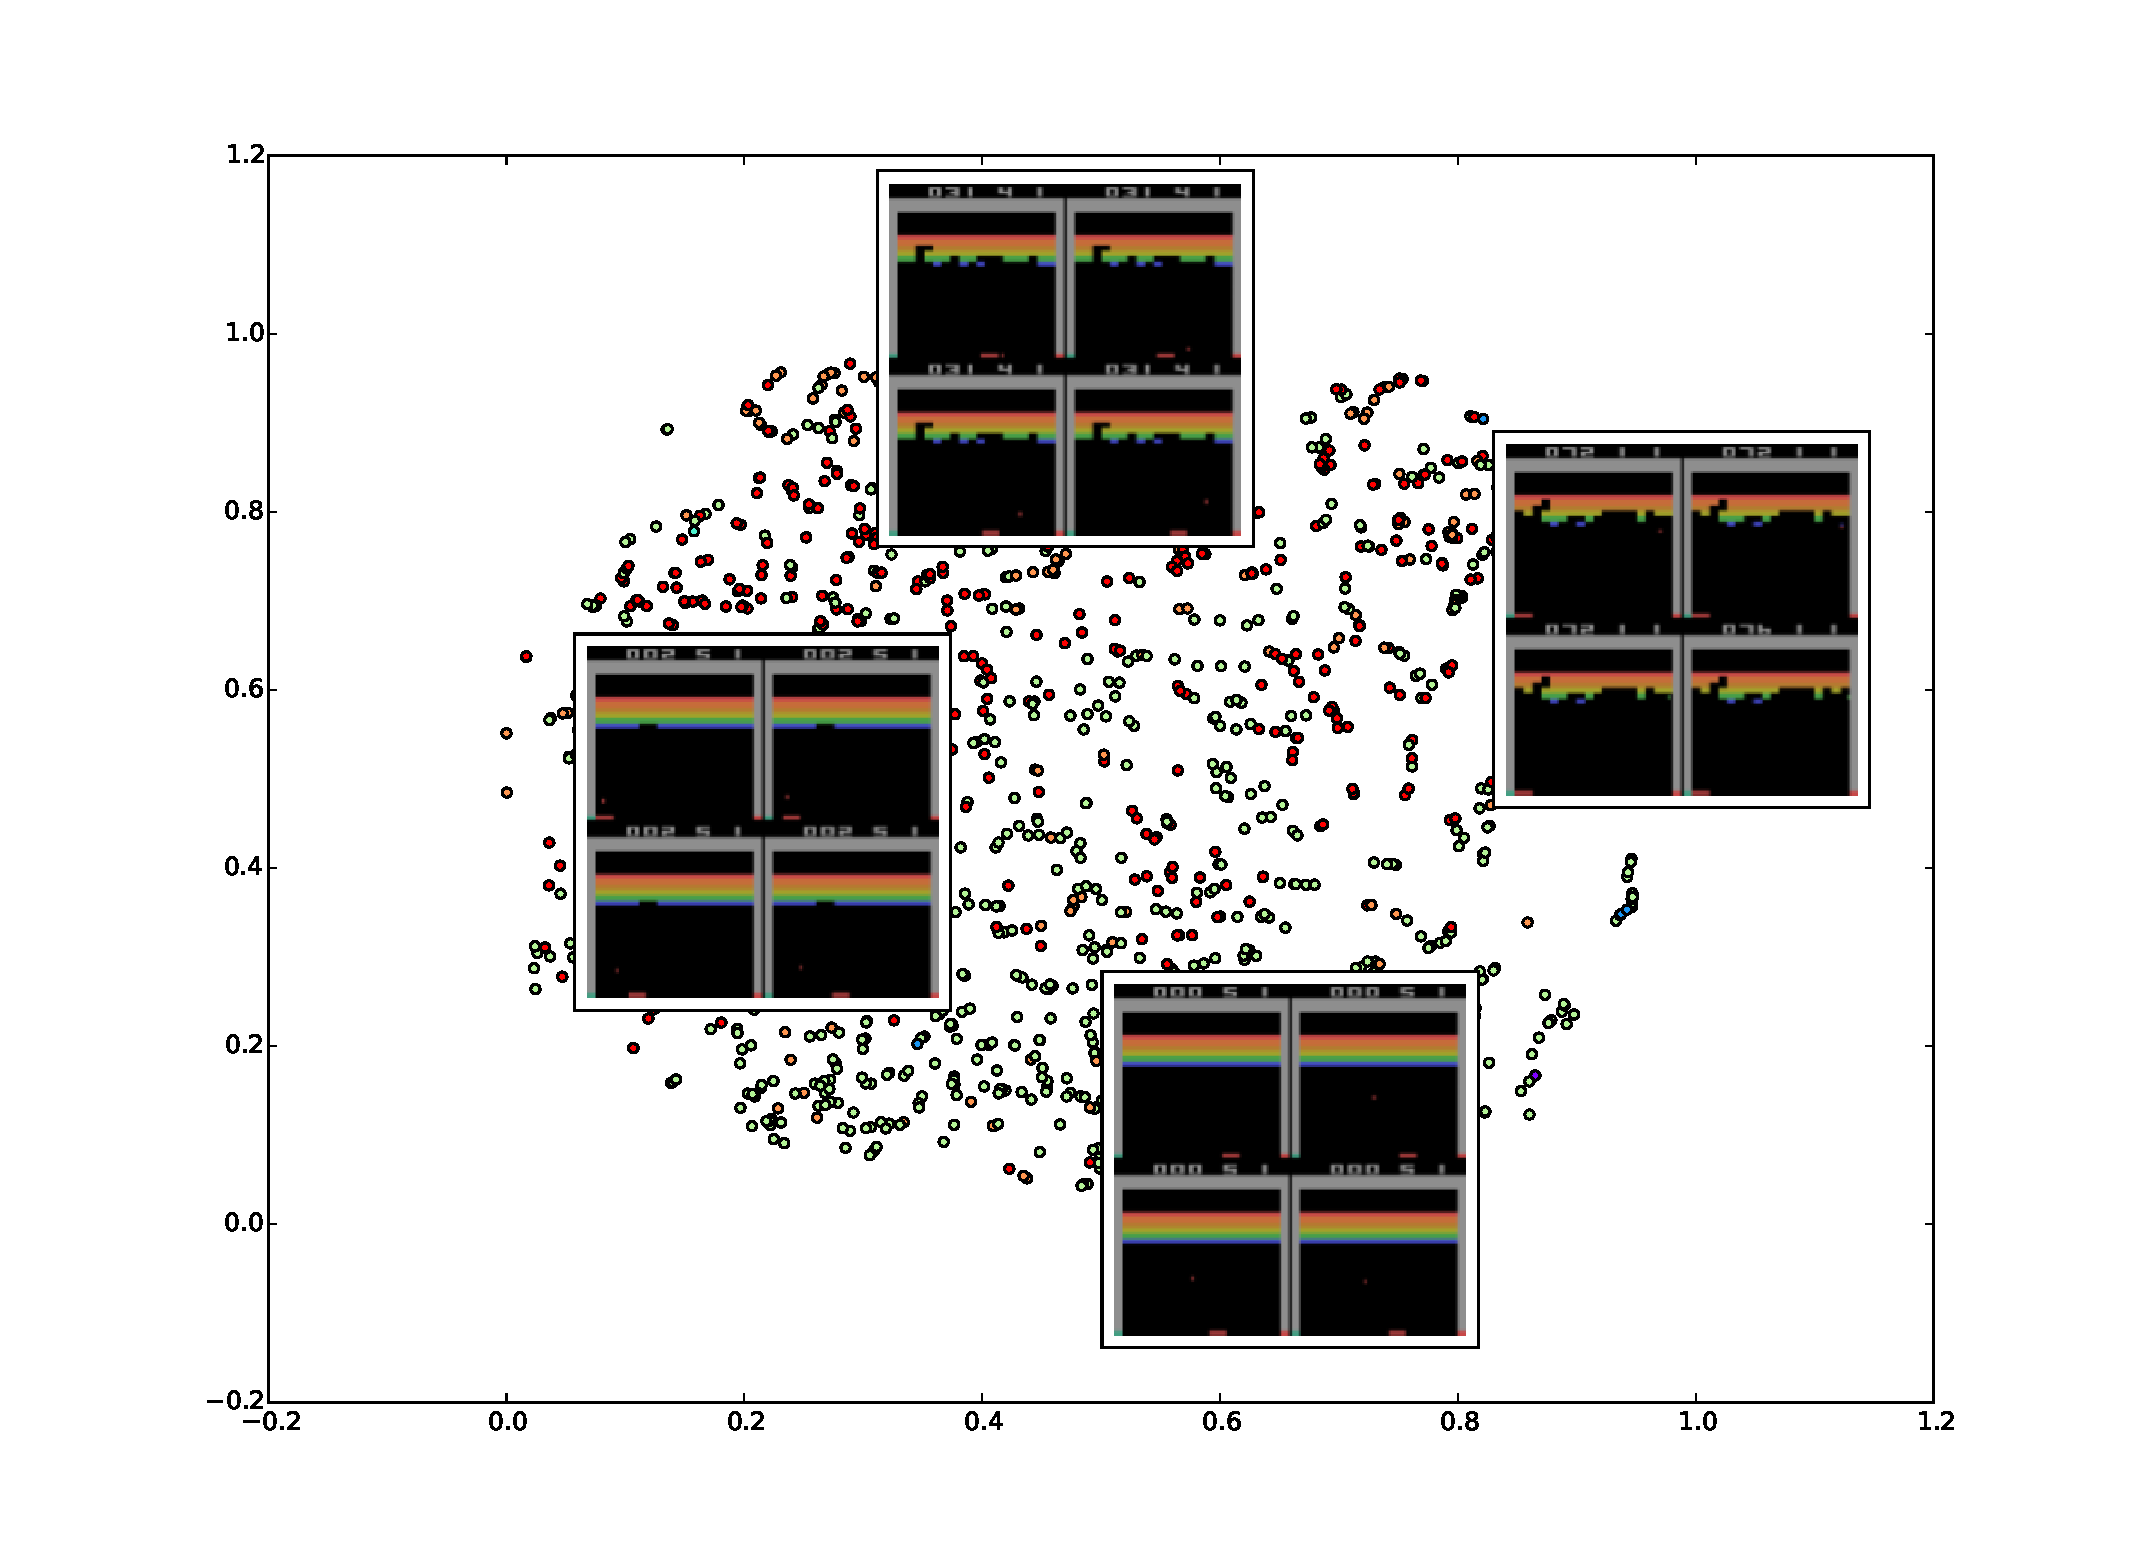
\includegraphics[width=1.1\textwidth, 
scale=0.8]{plots/tsne_breakout_new3_big.pdf}
 
 \caption[Fully connected layer's TSNE embedding in Deepmind's network]{The 
plot shows the TSNE embedding of the last fully connected layer in a network 
trained for the game of Breakout. The two primary colors--green and brown, 
respectively, show the two primary actions learned while playing the game of 
Breakout i.e. left and right respectively and the separation is almost 
apparent. }
\label{figure:deepmind-fc}
\end{figure}
Figure~\ref{figure:deepmind-fc} shows the last fully connected 
layer of a CNN trained to play Breakout trained using a reinforcement learning 
architecture. The separation between the state embeddings which are mapped to 
different actions is visible.\\

However, the deep reinforcement learning architecture in the work of 
\citet{deepmind_nips} performs poorly in deciding the optimal moves for games 
like Pacman etc. where the actions are best decided using a search or planning 
based method. Recently, an extension of this work by \citet*{guo2014deep} 
improved the results by a bit on some games that required extensive 
planning. Using a Monte-Carlo tree search based player to simulate trajectories, 
they trained a CNN based regression model on the generated state-action-value 
instances.\\

This integration of the CNN based RL agent and a planning 
agent having expert control motivates our case of modeling the complex dynamics 
of chess.

\section{Learning chess from scratch}
In this work, we undertake the task of learning to play the game of chess with 
minimal prior knowledge. The capability to learn chess, for our task, can be 
accomplished if a machine can:
\begin{itemize}
 \item Learn to play legal moves
 \item Rank the possible moves without any explicit guidance on relative
    importance of material or position. 
 \item Evaluate board positions
\end{itemize}

To accomplish this task using minimal knowledge prior, we use Convolutional 
neural networks to learn the game directly from board positions, moves and 
outcomes. We will finally evaluate our system on its ability to avoid illegal 
moves, predict good moves at certain board positions and play against a 
traditional search based chess player.\\

We believe that although such a system may not be able to play a championship 
level game, but it can prove to be an example of a chess player that has 
learned from scratch only observing chess games and having no clue of the 
rules.


\section{Aspects of expert human chess playing}
In this section, we look at what motivates us to solve the problem of chess playing as a 
pattern recognition task as opposed to the conventional approaches of 
accomplishing it as a predominantly search problem. We discuss various 
studies which suggest that most of the chess computer AIs that compete with the 
best human chess players don't probably play it the actual way humans do. 
Specifically, we motivate the task of playing chess in a more human way using a 
pattern recognition system in section~\ref{section:chess-as-pr}.\\

Adriaan de Groot, a Dutch chess master and a psychologist, after a deep 
statistical and interpretative analysis of chess players' transcripts of verbal 
utterances, their eye gaze movement and interviewing a number of beginner and 
master level chess players concluded that all players usually examine 40-50 
positions before playing a move. The difference however 
is that the master level players develop pattern recognition skills from 
experience which helps them examine only a few lines of play in much greater 
depth while ignoring the poor moves, where the beginners spend a lot of their 
time \cite{de1996perception}. Another evidence of why this is how humans 
play chess is that humans, especially at the master level, are capable of 
recognizing familiar arrangements of board or specific sets of pieces 
from experiences, rather than random arrangements of the same pieces  
\cite{chase1973perception}. Also unique to humans is the capability to learn 
from experience. This learning can both be ability to recognize patterns from 
the past games or it could be the ability to learn the weaknesses of the 
opponent or learn from his/her own strategic mistakes made.

\subsection{How to become an expert?}
\citet{ericsson2007making}, based on scientific research that 
looked at extraordinary and exceptional performance in a number of fields, 
observes that ``experts are always made, never born''. The author studied 
expertise in 
wide variety of domains ranging from chess to cooking, before concluding that 
the amount and quality of practice were the key factors in the level of 
performance achieved. The author also claims that a minimum of ten years of 
intense training is required before even the most gifted talents can 
win international competitions \cite{ericsson2006cambridge}. An aspect of this 
intense training and practice is that it is deliberate, meaning it 
consists of considerable and sustained efforts to do something which you can't 
already do well. The same goes for chess. Grandmasters, while they are very 
young, have played a huge number of games and also analyze the games they lost 
to eliminate all weaknesses in their gameplay.\\

Before Garry Kasparov, the then reigning world champion, was defeated by Deep 
Blue \cite{campbell2002deep} in May of 1997 in a chess match under tournament 
conditions, the two had a match in February 1996, when Kasparov came from 0-1 
down to win the match 4-2. The reason Kasparov could make a comeback was that 
he learned from Deep Blue's weaknesses and took advantage of them, while the 
deep blue computer responded similarly the next time too. This goes on to tell 
us the difference between a chess computer with no learning capability and a 
human grandmaster who learns about the weaknesses of the opponents. However, 
eventually Deep Blue was destined to beat Kasparov next year, but that was not 
an achieved because of a learning component, but more efficient and deeper 
search along with human intervention for tweaking the computer \cite{cnn-news}. 

\subsection{How are Grandmasters different?}
We associate the ability to play a good game of chess with someone's mental
ability-- such is the intellectual aura about chess. But 
\citet*{bilalic-mcleod-07_does-chess-need-intelligence_young-chess-players} 
suggests that better chess players do not necessarily perform exceptionally 
well in IQ tests. Further, neither are the chess grandmasters known to evaluate 
moves more rapidly then others \cite{de1996perception}. The aspects that mark 
chess grandmasters from others, appear to be similar to markers of expertise 
across a wide range of domains:
\begin{itemize}
 \item The mental representation is in terms of larger chunks, so that
	positions, and possible actions, are encoded more efficiently
	\cite{chase1973perception, gobet-clarkson-04memory_chunks}. In fact, 
the work by \citet*{deepmind_nips} shows that the representation learned by 
deep reinforcement learning architectures (shown in \ref{figure:deepmind-fc}) 
is arranged similarly i.e. states with similar actions are arranged in 
what may be called chunks.
\item Although a grandmaster may evaluate approximately the same number of
	moves as other players, the moves explored by the
	grandmaster are the stronger moves. Thus, presented with a board
	that may arise in a real chess game, the chess expert ``sees'' only a 
few good moves. This is also a type of pattern matching, but the 
complexity is mind-boggling. Perhaps this is possible 
only because the input space is no longer the set of distinct boards, but the 
space of all configurations of chunks, which is much smaller.
\end{itemize}


% \citet{gherrity1993game} introduced the notion of a general learning system, 
% known as the \textit{Search and Learning} system (SAL), that could learn to 
% play any rectangular board based two-player board game with a fixed types of 
% pieces. SAL, trained using temporal difference learning, learns from the 
% outcome of each game it plays. It was tested on Tic-tac-toe, Connect-4 and 
% Chess. It could successfully play Tic-tac-toe and Connect-4, but the level of 
% play he could achieve with a depth of search as 2 in chess was very poor. 
% However, this inspired works like Neurochess \cite{thrun1995learning} which used 
% chess game databases to learn the evaluation function while playing using a 
% standard search-based algorithm.

\subsection{Chess Reasoning as Pattern Recognition}
\label{section:chess-as-pr}
As we discussed above, the master level human chess players are known to 
recognize specific arrangements of the board or a specific set of pieces on the 
board and hence ignore certain poor positions to utilize their time to explore 
more important lines of play in a greater depth. We believe that an expert 
pattern recognition system, such as a human, would be able to recognize these 
patterns learned through experience and hence make a more informed decision to 
play a certain move. In other words, we think that a pattern recognition system 
that has seen enough examples of board positions and the corresponding expert 
moves should be able to predict favorable moves. But at the same time, we expect 
it to remain a necessity to explore those moves upto a greater depth.

% \section{Problem statement}
% In our work, we will take inspiration from these studies seeking a more human 
% way of playing the game of chess rather than computer chess 
% programs that predominantly employ search to make a move, which is a part of 
% what humans do before making a move. In fact, we try to solve a tougher 
% problem than just making a computer play chess well. We want the computer, 
% which has seen enough number of games, to figure out the rules of the game 
% without being explicitly programmed to know the rules of the game. By this 
% task, we also try to account for the generalization capabilities of a human 
% brain by looking at only a few examples of even a very vast set. For this task, 
% we make use of Convolutional neural networks which is a specific artificial 
% neural network architecture inspired by biological vision characteristically 
% suited for pattern recognition tasks (described in greater detail 
% in~\ref{subsection:cnn-background}). We want to emphasize that the our major 
% motivation is not to build a system that can beat other state of the art 
% systems, but to present a proof of concept that chess computers that are 
% inspired by human thinking and pattern recognition, as observed in the 
% case of grandmasters, can also yield a performance comparable to chess 
% programs that are predominantly based on search.


\section{Related work}
In the upcoming text, we will look at some of the related works in the 
fields of learning games using machine learning rather than logic and search. 
Some of the very recent works in combining deep learning with 
reinforcement learning has resulted in human level control of arcade 
games (discussed above). Many of these works have 
inspired us to take up Chess playing as machine learning and pattern recognition 
task. \\

\label{subsection:previous-works}
\subsection{Convolutional Neural Networks for playing Go}
Following the work of \citet{sutskever2008mimicking} which achieved modest 
success due to relatively small sized architecture, \citet{maddison2014move} 
used deep convolutional neural networks to play Go. The network could predict 
the correct move 55\% of the time and beat the traditional search program 
GnuGo in 97\% of the games without using any search and match the performance 
of a state-of-the-art Monte-Carlo tree search that simulates a million 
positions per move. They represent the current board position as a 3 channel 
image, along with adding channels for number of liberties before and after 
move, legality and the rank of the player. Much of the formulation of our 
model is motivated by this representation.\\

\subsection{Go versus Chess}
Using Convolutional networks to predict moves in Go proves to be a great step 
in the direction of building state of the art Go systems. This motivates us to 
use the same technique in predicting moves in the game of Chess. However, we 
must realize that the two games are fundamentally different in many aspects 
that make Go an easier game to play using a Convolutional Network. The game of 
Go has smoother arrangements of positions that are almost continuous 
within and between games.\\

Every move in Go adds a single piece to the board. 
Numerically speaking, making a move in Go using a random draw has a chance of 
$\frac{1}{361}$ on a $19\times 19$ board, while making a move drawing 
randomly the from and to positions in chess is correct with a 
chance of a mere $\frac{1}{4096}$. Also, a single move on a chess board makes a 
change of at least 2 pixels (more than 2 for a piece capture) which is 
significant for an $8\times 8$ board, while in Go only 1 pixel is added to the 
board every move making the transition much smoother than chess. Since, much 
of the knowledge of chess is characterized by strong domain knowledge in a 
logical form, such as ``if bishop on the central diagonal'', ``if the king has 
liberty more than 1'' etc., makes it less intuitive if as compared to the case 
of Go, Convolutional Neural networks can actually model the rules, leave 
aside the optimality of the moves.\\

\subsection{Deep learning for Chess}
This work also inspired a modest attempt of using convolutional neural networks 
to play chess, which achieved minimal success because of a much small dataset 
and weak representation \cite{oshripredicting}. We also acknowledge this work 
to have inspired us to make use of Convolutional neural networks to play chess. 
Other works that use deep learning to play chess do not learn the piece 
arrangements and their relative importances to score the table or evaluate it, 
rather they utilize a set of handcrafted features like king's safety, king's 
liberty, number of rooks on seventh rank etc. \cite{mannen2003learning, 
thrun1995learning} 

\subsection{Learning from Mistakes}
\label{subsection:mistakes-learn}
An important part of playing chess is to remember the each position in which 
the program made a mistake, so that the mistake is not repeated next time the 
position is encountered. The game playing system 
by \citet{epstein-01_learning-to-play-expertly-tutorial-on-hoyle} named HOYLE 
looks at the last position where the losing player could have made an alternate 
move by exhaustively searching the game tree. If the search succeeds, the 
alternate move is recorded and the state is marked as ``significant''. If the 
search fails to find an alternate path to winning position, the state is marked 
as ``dangerous''. In~\ref{subsection:representation-discussion-cnn}, we will 
look at how machine learning architectures like convolutional neural networks 
can provide more generalized representations, so that such ``significant'' and 
``dangerous'' states as well as other similar states are represented and 
searched for efficiently.

\section{Background}
\label{chap:background}
In this section, we will first look at what it means to play the game 
of chess perfectly, before moving on to studying how computers are programmed 
to play 
chess efficiently and exceptionally well. Further we look at some background 
about reinforcement learning, deep learning and 
learning representations and how 
convolutional neural networks, a specific case of deep learning architectures, 
has shaped the field of artificial intelligence especially in the area of 
pattern recognition.% in~\ref{subsection:cnn-background}. 
% In section~\ref{subsection:previous-works}, we also introduce some effective 
% approaches that solve problems similar to the task at hand like playing Atari 
% games using deep reinforcement learning, predicting moves in the games of Go 
and 
% evaluating moves in chess.  
\subsection{Ideal Leaf-evaluation function}
\label{section:solving}
Solving chess refers to finding an optimal strategy for playing chess. Chess 
has 
a finite number of states, estimated to be around $10^{43}$ 
by \citet{shannon1950xxii}. \citet{zermelo1913anwendung} proved that a 
hypothetically determinable optimal strategy does exist for chess.\\
In a weaker sense, each position can be assigned as a win for white, a win for 
Black or a forced draw if both the players are using the optimal strategy. We 
can formulate this as a function $f$ for each board position using the 
procedure 
below.
\begin{enumerate}
\item Assign all the positions with no further play possible as:
\[f(position) = \begin{cases}
1 \text{ , if White has won}\\
0 \text{ , if it is a draw}\\
-1 \text{ , if Black has won}
\end{cases}\]
\item Use the recursive rule up the game tree:
\[f(p) = \max\limits_{p\rightarrow p'} (-f(p'))\]
where $p'$ is a position reachable in one move from position $p$.\\
Here the negative sign means that a win for the opponent is a loss for the 
player in consideration and vice-versa.
\end{enumerate} 
The above recursive rule is the same as the minimax algorithm for the case when 
the game tree for chess is fully grown. The function $f$ gives us the 
``perfect'' evaluation function to play a chess game. While playing the game, 
we 
just need to choose the move which takes us to the board position $p$ for which 
$f(p)=1$.\\

But this evaluation function, $f$, cannot be computed with the computing 
resources available as of now. Hence, we need to resort to approximations of 
$f(p)$.


\subsection{Playing Chess using Computers}
\label{section:playing-background}
The first study on computers playing the game of chess was done by 
\citet{shannon1950xxii}. He predicted two main search strategies that would 
evolve with computers being programmed to play chess--
\begin{enumerate}
\item ``Type A" programs would use a ``brute force" examination of all the 
board 
positions possible through valid moves upto a certain depth of play.
\item ``Type B" programs would employ a ``quiescence search" looking at only a 
few good moves for each position. 
\end{enumerate}
He also predicted the ``Type A" programs to be impractical because of the 
massive search space. For even a computer evaluating $10^6$ moves per second, a 
lookahead of 3 moves for both sides, when an average of 30 moves are available 
for each board position, the program would take around 13 minutes.\\
\begin{table}[h]
\centering
%\resizebox{\textwidth}{!}
\caption{Time taken to explore 30 moves per position at $10^6$ moves per 
second.}
\label{table:time-taken}
\end{table}

However, with the exponential increase in the computation power since then, the 
most successful methods for playing chess are programmed to use ``Type A" 
programs. One reason for ignoring ``Type B'' is that relying on the board 
configuration to decide on the moves to explore is a much harder problem than 
using a faster, yet weaker, evaluation metric for a larger depth. It is widely 
believed that a faster evaluation function with an efficient search along with 
heuristic pruning would build a better chess playing computer than the one that 
uses a better but slower evaluation function that involves pattern recognition 
techniques similar to our brain.

\subsection{Conventional Chess Playing Computers}
\label{subsection:conventional-chess}
The fundamental implementation details of chess-playing computer system include:
\begin{itemize}
\item \textbf{Board Representation} -- how a board position is represented in a 
data structure. The performance of move generation and piece evaluation depends 
on the data structure used to represent the board position. The most common 
representation uses a list of piece positions for each position. Some of the 
other methods are-- mailbox, 0x88, bitboards and huffman codes. We will discuss 
the representation used for our training and playing tasks in Chapter 
\ref{chap:dataset}.

\item \textbf{Search Techniques} -- how to identify and select the moves for 
further evaluation. Some of the most widely used search techniques are-- 
Minmax, Negamax, Negascout, Iterative deepening depth-first search etc. Much of 
the 
focus on state of the art chess playing systems resides on making search more 
efficient to evaluate more board positions per unit time. One of these 
algorithms which we make use of is Negamax algorithm and has 
been explained in section~\ref{subsection:interleaved}.

\item\textbf{Leaf Evaluation} -- how to evaluate the position of the board if 
no 
further evaluation needs to be done. The mapping from a board to an integer 
value is called the evaluation function. An evaluation function typically 
considers material value along with other factors affecting the strength of 
play for each player. The most common values for materials is 1 point for pawn, 
3 for bishop, 3 for knight, 5 for rook, 9 for queen and 200 for king. The high 
value for king ensures that checkmate outweighs everything. The sum of the 
values for all material on the board with negative weights to the opponent is 
the evaluation of the table. In addition to pieces, most evaluation functions 
take into consideration more factors like pawn structure, pair of bishops, 
protection of the king etc.
\end{itemize}


\subsection{Reinforcement Learning}
\label{section:RL}
The fundamental principle behind all Reinforcement learning methods is that we 
use the current policy, run it on the environment, observe the feedback and 
make the good outcomes more likely, the bad outcomes less likely. Reinforcement 
learning differs from standard supervised learning in the way that an RL 
algorithm is not presented with optimal actions to input states 
\cite{sutton1998reinforcement}. The basic reinforcement learning model contains 
the following components:
\begin{enumerate}
 \item a set of environment states $\mathcal{S}$
 \item a set of actions $\mathcal{A}$
 \item transition rules between states
 \item rules that determine the \textit{scalar intermediate reward} of a 
transition
\item rules that describe what the agent observes
\end{enumerate}
However it is a very hard problem to do a policy search using a reinforcement 
learning architecture when we have a combination of complex dynamics and 
complex policy. The high dimensionality of such policies doesn't allow 
efficient policy search. However, there have been successful attempts to 
convert these complex dynamics and complex policy domain problems to only a 
complex policy problem by decomposing the policy search into two phases-- 
optimal control and supervised learning \cite{levine2015end}. The end to end 
training for the supervised learning part is done using a function 
approximator, convolutional neural networks in our case, which we will 
discuss in section~\ref{subsection:cnn-background}. 
Other attempts to combine conventional reinforcement learning techniques with 
deep learning to learn optimal control have yielded near human performance on 
tasks like playing Atari video games \cite{deepmind_nips}. The task that 
representation learning architectures like CNNs solve is the problem of 
perception i.e. the feature representation of the states need not be 
composed of hand-crafted features, but can be learned while training.

\subsection{Deep Learning}
\label{section:dl-background}
The area of Neural Networks has been inspired by the aim of modeling biological 
neural systems. Although it has diverged from this aim since then, the basic 
computational unit in an artificial neural network still remains a neuron, 
which takes the signal from the axons from other neurons as inputs, 
with dendrites carrying the signal to the nucleus where it gets summed up and 
the neuron is activated if the sum is above some threshold. Such a neuron can 
be represented mathematically as: $f(\sum_i w_ix_i + b)$, where $f$ is the 
activation function, $w_i$ is the weight given to the input from one of its 
dendrites. In other words, a neuron computes the dot product of its weights and 
the inputs, adds the bias and applies an activation function. A mathematical 
model of a neuron is shown in the figure below.
\begin{figure}[H]
\begin{tikzpicture}[
init/.style={
  draw,
  circle,
  inner sep=2pt,
  font=\Huge,
  join = by -latex
},
squa/.style={
  draw,
  inner sep=2pt,
  font=\Large,
  join = by -latex
},
start chain=2,node distance=13mm
]
\node[on chain=2] 
  (x2) {$x_2$};
\node[on chain=2,join=by o-latex] 
  {$w_2$};
\node[on chain=2,init] (sigma) 
  {$\displaystyle\Sigma$};
\node[on chain=2,squa,label=above:{\parbox{2cm}{\centering Activate \\ 
function}}]   
  {$f$};
\node[on chain=2,label=above:Output,join=by -latex] 
  {$y$};
\begin{scope}[start chain=1]
\node[on chain=1] at (0,1.5cm) 
  (x1) {$x_1$};
\node[on chain=1,join=by o-latex] 
  (w1) {$w_1$};
\end{scope}
\begin{scope}[start chain=3]
\node[on chain=3] at (0,-1.5cm) 
  (x3) {$x_3$};
\node[on chain=3,label=below:Weights,join=by o-latex] 
  (w3) {$w_3$};
\end{scope}
\node[label=above:\parbox{2cm}{\centering Bias \\ $b$}] at (sigma|-w1) (b) {};

\draw[-latex] (w1) -- (sigma);
\draw[-latex] (w3) -- (sigma);
\draw[o-latex] (b) -- (sigma);

\draw[decorate,decoration={brace,mirror}] (x1.north west) -- node[left=10pt] 
{Inputs} (x3.south west);
\end{tikzpicture}
\caption{An artificial neuron as a mathematical model}
\end{figure}

Neural networks are the collections of neurons that are connected in an acyclic 
graph. This means that outputs of some set of neurons becomes the input of 
another set of neurons. The most common arrangement is a layered neural network 
with an input and an output layer, along with none or more hidden layers. 
The input layer has number of neurons equal to the input dimension and the 
number of output layer neurons is the dimension of the output. The hidden 
layers can contain different numbers of neurons. A two-layer neural network is 
shown in the figure below. The two-layer here refers to the number of layers 
besides the input layer.
\begin{figure}[H]
\begin{tikzpicture}[
plain/.style={
  draw=none,
  fill=none,
  },
net/.style={
  matrix of nodes,
  nodes={
    draw,
    circle,
    inner sep=10pt
    },
  nodes in empty cells,
  column sep=2cm,
  row sep=-9pt
  },
>=latex
]
\matrix[net] (mat)
{
|[plain]| \parbox{1.3cm}{\centering Input\\layer} & |[plain]| 
\parbox{1.3cm}{\centering Hidden\\layer} & |[plain]| \parbox{1.3cm}{\centering 
Output\\layer} \\
& |[plain]| \\
|[plain]| & \\
& |[plain]| \\
|[plain]| & |[plain]| \\
& & \\
|[plain]| & |[plain]| \\
& |[plain]| \\
|[plain]| & \\
& |[plain]| \\
};
\foreach \ai [count=\mi ]in {2,4,...,10}
  \draw[<-] (mat-\ai-1) -- node[above] {Input \mi} +(-2cm,0);
\foreach \ai in {2,4,...,10}
{\foreach \aii in {3,6,9}
  \draw[->] (mat-\ai-1) -- (mat-\aii-2);
}
\foreach \ai in {3,6,9}
  \draw[->] (mat-\ai-2) -- (mat-6-3);
\draw[->] (mat-6-3) -- node[above] {Ouput} +(2cm,0);
\end{tikzpicture}
\caption{A two layer Artificial Neural network}
\end{figure}

In practice, we model a real valued function using a multi-layer neural 
network. This real valued function, for example, is the one which outputs the 
class value in case of a classification task or a continuous function in case 
of a regression task. In other words, a multi-layer artificial neural 
network defines a family of functions parameterized by the weights of the 
network. By learning the weights of such a network we usually means learning a 
function belonging to this family of functions that best represents the 
training 
data.

\subsection{Universal Approximation Properties of Multilayer Perceptrons}
\label{subsection:universal-approx}
We discussed above that a family of functions is represented by a single 
artificial neural network with fixed architecture. It has been proved that 
Neural networks with at least one hidden layer are universal 
approximators \cite{hornik1989multilayer}. This means that given any continuous 
function $f(x)$ and some $\epsilon>0$, a Neural network with one hidden layer 
containing a sufficient number of hidden layer neurons and a suitable choice of 
non-linearity, say represented by $g(x)$, exists such that $\forall x, 
|f(x)-g(x)|<\epsilon$. In other words, we can approximate any given real 
valued continuous function with a two layer Neural network upto a certain 
accuracy.\\

The fact that two layer Neural networks are universal approximators 
is a pretty useless property in the case of machine learning. Neither does it 
tell the number of hidden units required to represent a given function upto the 
desired precision, nor does it promise that it represents a generalized 
function 
that fits the unseen data. The generalized function is expected to be smooth, 
while the overly precise two-layer network may overfit for the input data and 
not learn a promising representation.

\subsection{Representation Learning}
\label{subsection:representation}
We learnt that despite being universal approximators, it may not reasonable to 
approximate a function for a task at hand using two-layer Neural networks 
because of insufficient generalization ability. Meanwhile, a lot of 
experimental evidence from the recent past shows that these functions can be 
learnt to a greater generalization using Neural networks of larger depths 
\cite{bengio-dl-book}. Most of these works involve using a specific class of 
Neural networks architectures, namely Convolutional Neural Networks, which we 
will discuss in section \ref{subsection:cnn-background}. This leads us to 
believe that depth indeed is a useful consideration to make while choosing a 
Neural network architecture to fit data, and it provides the learner's family 
of functions multiple levels of representation and hence making the function 
smoother yielding better generalization. 

\subsection{Convolutional Neural Networks}
\label{subsection:cnn-background}
Convolutional neural networks, sometimes referred to as Convolutional Networks 
or ConvNets, is a particular architecture of deep neural networks inspired 
by the seminal work by \citet{hubel1963shape} on feedforward processing in 
early visual cortex. The architecture uses hierarchical layers of tiled 
convolutional filters to mimic the effects of receptive fields. These filters 
exploit the local spatial correlations present in the images. In 
practice, these hierarchical layers are alternated with subsampling layers like 
max-pool and a non-linearity map, and further connected to fully connected 
layers just like in other deep learning architectures and the full 
network is trained using back propagation. In short, Convolutional neural 
networks are nothing but neural networks which use convolution instead of 
full matrix multiplications in atleast one of the layers \cite{bengio-dl-book}. 
\\
\begin{figure}[H]
\centering
\begin{tikzpicture}

				\node at (0.5,-0.75){\begin{tabular}{c}input 
image\end{tabular}};
		
				\draw (0,0) -- (1,0) -- (1,1) -- (0,1) -- (0,0);
		
				\node at 
(3,3.25){\begin{tabular}{c}convolutional layer\\with 
non-linearities\end{tabular}};
		
				\draw[fill=black,opacity=0.2,draw=black] 
(2.75,1.25) -- (3.75,1.25) -- (3.75,2.25) -- (2.75,2.25) -- (2.75,1.25);
				\draw[fill=black,opacity=0.2,draw=black] 
(2.5,1) 
-- (3.5,1) -- (3.5,2) -- (2.5,2) -- (2.5,1);
				\draw[fill=black,opacity=0.2,draw=black] 
(2.25,0.75) -- (3.25,0.75) -- (3.25,1.75) -- (2.25,1.75) -- (2.25,0.75);
				\draw[fill=black,opacity=0.2,draw=black] 
(2,0.5) 
-- (3,0.5) -- (3,1.5) -- (2,1.5) -- (2,0.5);
				\draw[fill=black,opacity=0.2,draw=black] 
(1.75,0.25) -- (2.75,0.25) -- (2.75,1.25) -- (1.75,1.25) -- (1.75,0.25);
				\draw[fill=black,opacity=0.2,draw=black] 
(1.5,0) 
-- (2.5,0) -- (2.5,1) -- (1.5,1) -- (1.5,0);
		
				\node at 
(4.5,-0.75){\begin{tabular}{c}subsampling layer\end{tabular}};
		
				\draw[fill=black,opacity=0.2,draw=black] 
(5,1.25) -- (5.75,1.25) -- (5.75,2) -- (5,2) -- (5,1.25);
				\draw[fill=black,opacity=0.2,draw=black] 
(4.75,1) -- (5.5,1) -- (5.5,1.75) -- (4.75,1.75) -- (4.75,1);
				\draw[fill=black,opacity=0.2,draw=black] 
(4.5,0.75) -- (5.25,0.75) -- (5.25,1.5) -- (4.5,1.5) -- (4.5,0.75);
				\draw[fill=black,opacity=0.2,draw=black] 
(4.25,0.5) -- (5,0.5) -- (5,1.25) -- (4.25,1.25) -- (4.25,0.5);
				\draw[fill=black,opacity=0.2,draw=black] 
(4,0.25) -- (4.75,0.25) -- (4.75,1) -- (4,1) -- (4,0.25);
				\draw[fill=black,opacity=0.2,draw=black] 
(3.75,0) -- (4.5,0) -- (4.5,0.75) -- (3.75,0.75) -- (3.75,0);
		
% %				\node at 
% (7,3.5){\begin{tabular}{c}convolutional 
% layer\\with non-linearities\\layer $l = 4$\end{tabular}};
% %		
% %				\draw[fill=black,opacity=0.2,draw=black] 
% (7.5,1.75) -- (8.25,1.75) -- (8.25,2.5) -- (7.5,2.5) -- (7.5,1.75);
% %				\draw[fill=black,opacity=0.2,draw=black] 
% (7.25,1.5) -- (8,1.5) -- (8,2.25) -- (7.25,2.25) -- (7.25,1.5);
% %				\draw[fill=black,opacity=0.2,draw=black] 
% (7,1.25) -- (7.75,1.25) -- (7.75,2) -- (7,2) -- (7,1.25);
% %				\draw[fill=black,opacity=0.2,draw=black] 
% (6.75,1) -- (7.5,1) -- (7.5,1.75) -- (6.75,1.75) -- (6.75,1);
% %				\draw[fill=black,opacity=0.2,draw=black] 
% (6.5,0.75) -- (7.25,0.75) -- (7.25,1.5) -- (6.5,1.5) -- (6.5,0.75);
% %				\draw[fill=black,opacity=0.2,draw=black] 
% (6.25,0.5) -- (7,0.5) -- (7,1.25) -- (6.25,1.25) -- (6.25,0.5);
% %				\draw[fill=black,opacity=0.2,draw=black] 
% (6,0.25) -- (6.75,0.25) -- (6.75,1) -- (6,1) -- (6,0.25);
% %				\draw[fill=black,opacity=0.2,draw=black] 
% (5.75,0) -- (6.5,0) -- (6.5,0.75) -- (5.75,0.75) -- (5.75,0);
% %		
% %				\node at (9.5,-1){\begin{tabular}{c}subsampling 
% layer\\layer $l = 6$\end{tabular}};
% 		
% %				\draw[fill=black,opacity=0.2,draw=black] 
% (10,1.75) -- (10.5,1.75) -- (10.5,2.25) -- (10,2.25) -- (10,1.75);
% %				\draw[fill=black,opacity=0.2,draw=black] 
% (9.75,1.5) -- (10.25,1.5) -- (10.25,2) -- (9.75,2) -- (9.75,1.5);
% %				\draw[fill=black,opacity=0.2,draw=black] 
% (9.5,1.25) -- (10,1.25) -- (10,1.75) -- (9.5,1.75) -- (9.5,1.25);
% %				\draw[fill=black,opacity=0.2,draw=black] 
% (9.25,1) -- (9.75,1) -- (9.75,1.5) -- (9.25,1.5) -- (9.25,1);
% %				\draw[fill=black,opacity=0.2,draw=black] 
% (9,0.75) -- (9.5,0.75) -- (9.5,1.25) -- (9,1.25) -- (9,0.75);
% %				\draw[fill=black,opacity=0.2,draw=black] 
% (8.75,0.5) -- (9.25,0.5) -- (9.25,1) -- (8.75,1) -- (8.75,0.5);
% %				\draw[fill=black,opacity=0.2,draw=black] 
% (8.5,0.25) -- (9,0.25) -- (9,0.75) -- (8.5,0.75) -- (8.5,0.25);
% %				\draw[fill=black,opacity=0.2,draw=black] 
% (8.25,0) -- (8.75,0) -- (8.75,0.5) -- (8.25,0.5) -- (8.25,0);
% 		
				\node at (6.5,1){$\ldots$};
		
				\node at (8.5,3.25){\begin{tabular}{c}two-layer 
perceptron\end{tabular}};
		
				\draw[fill=black,draw=black,opacity=0.5] 
(6.5,0) 
-- (7,0) -- (8.5,1.75) -- (8,1.75) -- (6.5,0);
		
% 				%\node at (9,-1){\begin{tabular}{c}fully 
% connected layer\\output layer $l = 8$\end{tabular}};
		
				\draw[fill=black,draw=black,opacity=0.5] 
(8.5,0.5) -- (9,0.5) -- (9.65,1.25) -- (9.15,1.25) -- (8.5,0.5);
\end{tikzpicture}
\caption{A typical Convolutional Neural Network architecture}			
\end{figure}		
		
Convolutional Neural Networks have brought about a revolution in computer 
vision and is now the most successful approach for almost all recognition and 
detection tasks in computer vision 
\cite{krizhevsky2012imagenet,tompson2014efficient,taigman2014deepface} 
and some even approach human performance on some tasks 
\cite{ciresan2012multi}.\\

\subsubsection{Utilizing CNN's representation power}
\label{subsection:representation-discussion-cnn}
In~\ref{subsection:mistakes-learn}, we looked at a heuristic based game playing 
system called 
HOYLE~\cite{epstein-01_learning-to-play-expertly-tutorial-on-hoyle} that 
recorded a set of ``significant'' and ``dangerous'' states by exhaustively 
searching the tree, starting from states to look for alternate paths to win, 
whenever a game is lost. It is easy to understand that this system is not 
scalable to learning from a large set of games and neither can the applicability 
be explained with a small number of recorded states. However, the 
representation power of the convolutional neural networks can help in the 
representation of these ``dangerous'' and ``significant'' states. For instance, 
the first fully connected layer represents a n-dimensional space in which the 
similar states are embedded closer. This can significantly contribute to the 
HOYLE's strategy by providing a better generalization and efficient 
representation to the recorded states.

%XXX Describe this work in greater detail.

% \subsubsection{Playing Arcade Games using Convolutional Neural Networks}
% \label{subsubsection:deepmind}
% A remarkable work that helped bridge the gap between perception and action has 
% been Deepmind's deep reinforcement learning agent that is capable of learning 
% human-level control from high dimensional sensory input of an Atari video game 
% \cite{deepmind_nips}.\\
% 
% We tried to explore the last fully connected layer of a 
% convolutional neural network trained to play Breakout. The 
% figure~\ref{figure:deepmind} shows the apparent separation between the state 
% embeddings which are mapped to different actions.\\
% 
% \begin{figure}[h]
%  \centering
%  \hspace*{-1.2in}
%  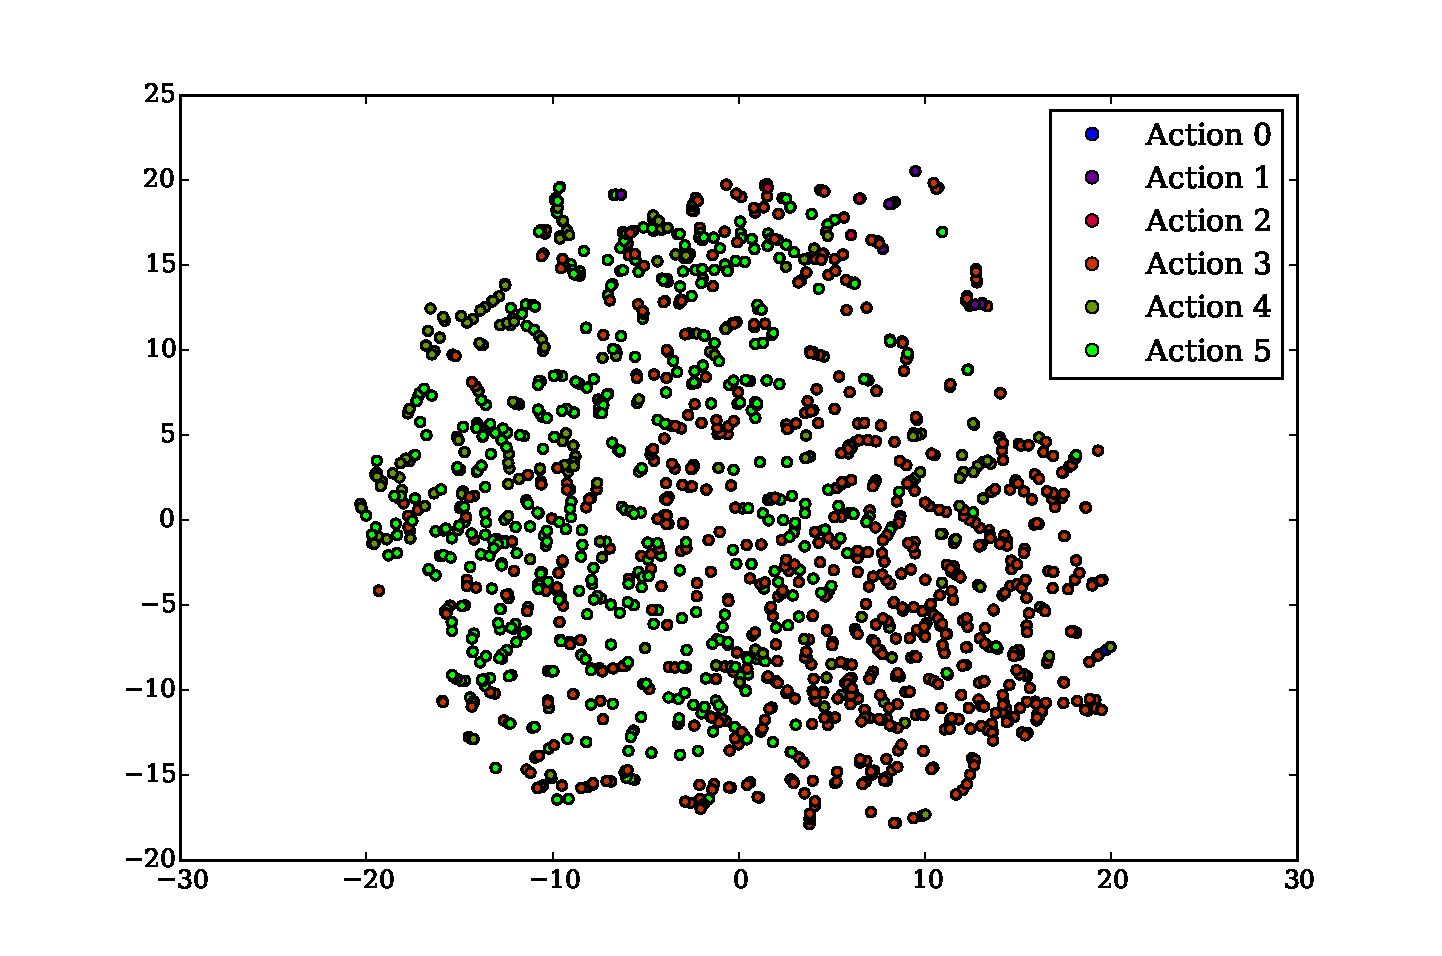
\includegraphics[width=1.5\textwidth]{plots/tsne_breakout_new.pdf}
%  
%  \caption[Fully connected layer's TSNE embedding in Deepmind's network]{The 
% plot shows the TSNE embedding of the last fully connected layer in a network 
% trained for the game of Breakout. The two primary colors--green and brown, 
% respectively, show the two primary actions learned while playing the game of 
% Breakout i.e. left and right respectively and the separation is almost 
% apparent. }
% \label{figure:deepmind}
% \end{figure}
% 
% 
% An extension of this work by \citet*{guo2014deep} 
% improved the results a bit on some games that required extensive planning. They 
% used a Monte-Carlo tree search based player to simulate trajectories, before 
% using the generated state-action-value instances to train a CNN based 
% regression model. The method proved to make a fruitful integration of a 
% planning agent and the RL agent in a way similar to the one discussed 
% in section~\ref{section:RL}.\\ 
% 
% Along with the TSNE embedding in figure~\ref{figure:deepmind}, builds our 
% intuition that the subspace that the convolutional neural network embeds the 
% state representations (i.e. the game screens) in Breakout on the basis of the 
% most favorable action for that state. We will see that 
% regardless of the task specification i.e. either we choose Q-learning (e.g. in 
% \citet{deepmind_nips}) or we choose a regression or classification task (e.g. 
% in \citet{guo2014deep}), we are almost asking the network to embed the states 
% effectively to select the best action.\\
% 
% This is the major motivation to our method of learning the evaluation 
% function for chess boards (state) based on the final outcome of the games, 
% which we describe in the next chapter.

\section*{Organization of the thesis}
The thesis is organized in the classic style of first introducing the problem 
and discussing related work (chapter~\ref{chap:introduction}), 
then chapter~\ref{chap:implementation} where we describe 
our dataset representation and implementation details while 
systematically moving towards our aim. Finally we present the results and 
analysis (chapter~\ref{chap:results}). In the chapter~\ref{chap:implementation}, 
we specifically mention the convolutional neural network architecture we use, 
the loss functions and the how we employ them to choose a move while playing a 
game of chess. In the results chapter, we describe the strengths and weaknesses 
of our system by considering specific case studies. Finally, we conclude with a 
discussion about the feasibility of such systems and how they can be a part of 
the future of computer chess.
% 	\chapter{Background}
\label{chap:background}
In this chapter, we will first look at what it means to actually solve the game 
of chess, before moving on to studying how computers are programmed to play 
chess efficiently and exceptionally well. Further we look at some background 
about reinforcement learning, deep learning and 
learning representations and how 
convolutional neural networks, a specific case of deep learning architectures, 
has shaped the field of artificial intelligence especially in the area of 
pattern recognition.% in~\ref{subsection:cnn-background}. 
% In section~\ref{subsection:previous-works}, we also introduce some effective 
% approaches that solve problems similar to the task at hand like playing Atari 
% games using deep reinforcement learning, predicting moves in the games of Go and 
% evaluating moves in chess.  
\section*{Solving Chess}
\label{section:solving}
Solving chess refers to finding an optimal strategy for playing chess. Chess has 
a finite number of states, estimated to be around $10^{43}$ 
by \citet{shannon1950xxii}. \citet{zermelo1913anwendung} proved that a 
hypothetically determinable optimal strategy does exist for chess.\\
In a weaker sense, each position can be assigned as a win for white, a win for 
Black or a forced draw if both the players are using the optimal strategy. We 
can formulate this as a function $f$ for each board position using the procedure 
below.
\begin{enumerate}
\item Assign all the positions with no further play possible as:
\[f(position) = \begin{cases}
1 \text{ , if White has won}\\
0 \text{ , if it is a draw}\\
-1 \text{ , if Black has won}
\end{cases}\]
\item Use the recursive rule up the game tree:
\[f(p) = \max\limits_{p\rightarrow p'} (-f(p'))\]
where $p'$ is a position reachable in one move from position $p$.\\
Here the negative sign means that a win for the opponent is a loss for the 
player in consideration and vice-versa.
\end{enumerate} 
The above recursive rule is the same as the minimax algorithm for the case when 
the game tree for chess is fully grown. The function $f$ gives us the 
``perfect'' evaluation function to play a chess game. While playing the game, we 
just need to choose the move which takes us to the board position $p$ for which 
$f(p)=1$.\\

But this evaluation function, $f$, cannot be computed with the computing 
resources available as of now. Hence, we need to resort to approximations of 
$f(p)$.


\section*{Playing Chess using Computers}
\label{section:playing-background}
The first study on computers playing the game of chess was done by 
\citet{shannon1950xxii}. He predicted two main search strategies that would 
evolve with computers being programmed to play chess--
\begin{enumerate}
\item ``Type A" programs would use a ``brute force" examination of all the board 
positions possible through valid moves upto a certain depth of play.
\item ``Type B" programs would employ a ``quiescence search" looking at only a 
few good moves for each position. 
\end{enumerate}
He also predicted the ``Type A" programs to be impractical because of the 
massive search space. For even a computer evaluating $10^6$ moves per second, a 
lookahead of 3 moves for both sides, when an average of 30 moves are available 
for each board position, the program would take around 13 minutes.\\
\begin{table}[h]
\centering
%\resizebox{\textwidth}{!}
\caption{Time taken to explore 30 moves per position at $10^6$ moves per 
second.}
\label{table:time-taken}
\end{table}

However, with the exponential increase in the computation power since then, the 
most successful methods for playing chess are programmed to use ``Type A" 
programs. One reason for ignoring ``Type B'' is that relying on the board 
configuration to decide on the moves to explore is a much harder problem than 
using a faster, yet weaker, evaluation metric for a larger depth. It is widely 
believed that a faster evaluation function with an efficient search along with 
heuristic pruning would build a better chess playing computer than the one that 
uses a better but slower evaluation function that involves pattern recognition 
techniques similar to our brain.

\subsection*{Conventional Chess Playing Computers}
\label{subsection:conventional-chess}
The fundamental implementation details of chess-playing computer system include:
\begin{itemize}
\item \textbf{Board Representation} -- how a board position is represented in a 
data structure. The performance of move generation and piece evaluation depends 
on the data structure used to represent the board position. The most common 
representation uses a list of piece positions for each position. Some of the 
other methods are-- mailbox, 0x88, bitboards and huffman codes. We will discuss 
the representation used for our training and playing tasks in Chapter 
\ref{chap:dataset}.

\item \textbf{Search Techniques} -- how to identify and select the moves for 
further evaluation. Some of the most widely used search techniques are-- 
Minmax, Negamax, Negascout, Iterative deepening depth-first search etc. Much of 
the 
focus on state of the art chess playing systems resides on making search more 
efficient to evaluate more board positions per unit time. One of these 
algorithms which we make use of is Negamax algorithm and has 
been explained in section~\ref{subsection:interleaved}.

\item\textbf{Leaf Evaluation} -- how to evaluate the position of the board if 
no 
further evaluation needs to be done. The mapping from a board to an integer 
value is called the evaluation function. An evaluation function typically 
considers material value along with other factors affecting the strength of 
play for each player. The most common values for materials is 1 point for pawn, 
3 for bishop, 3 for knight, 5 for rook, 9 for queen and 200 for king. The high 
value for king ensures that checkmate outweighs everything. The sum of the 
values for all material on the board with negative weights to the opponent is 
the evaluation of the table. In addition to pieces, most evaluation functions 
take into consideration more factors like pawn structure, pair of bishops, 
protection of the king etc.
\end{itemize}


\section*{Reinforcement Learning}
\label{section:RL}
The fundamental principle behind all Reinforcement learning methods is that we 
use the current policy, run it on the environment, observe the feedback and 
make the good outcomes more likely, the bad outcomes less likely. Reinforcement 
learning differs from standard supervised learning in the way that an RL 
algorithm is not presented with optimal actions to input states 
\cite{sutton1998reinforcement}. The basic reinforcement learning model contains 
the following components:
\begin{enumerate}
 \item a set of environment states $\mathcal{S}$
 \item a set of actions $\mathcal{A}$
 \item transition rules between states
 \item rules that determine the \textit{scalar intermediate reward} of a 
transition
\item rules that describe what the agent observes
\end{enumerate}
However it is a very hard problem to do a policy search using a reinforcement 
learning architecture when we have a combination of complex dynamics and 
complex policy. The high dimensionality of such policies doesn't allow 
efficient policy search. However, there have been successful attempts to 
convert these complex dynamics and complex policy domain problems to only a 
complex policy problem by decomposing the policy search into two phases-- 
optimal control and supervised learning \cite{levine2015end}. The end to end 
training for the supervised learning part is done using a function 
approximator, convolutional neural networks in our case, which we will 
discuss in section~\ref{subsection:cnn-background}. 
Other attempts to combine conventional reinforcement learning techniques with 
deep learning to learn optimal control have yielded near human performance on 
tasks like playing Atari video games \cite{deepmind_nips}. The task that 
representation learning architectures like CNNs solve is the problem of 
perception i.e. the feature representation of the states need not be 
composed of hand-crafted features, but can be learned while training.

\section*{Deep Learning}
\label{section:dl-background}
The area of Neural Networks has been inspired by the aim of modeling biological 
neural systems. Although it has diverged from this aim since then, the basic 
computational unit in an artificial neural network still remains a neuron, 
which takes the signal from the axons from other neurons as inputs, 
with dendrites carrying the signal to the nucleus where it gets summed up and 
the neuron is activated if the sum is above some threshold. Such a neuron can 
be represented mathematically as: $f(\sum_i w_ix_i + b)$, where $f$ is the 
activation function, $w_i$ is the weight given to the input from one of its 
dendrites. In other words, a neuron computes the dot product of its weights and 
the inputs, adds the bias and applies an activation function. A mathematical 
model of a neuron is shown in the figure below.
\begin{figure}[H]
\begin{tikzpicture}[
init/.style={
  draw,
  circle,
  inner sep=2pt,
  font=\Huge,
  join = by -latex
},
squa/.style={
  draw,
  inner sep=2pt,
  font=\Large,
  join = by -latex
},
start chain=2,node distance=13mm
]
\node[on chain=2] 
  (x2) {$x_2$};
\node[on chain=2,join=by o-latex] 
  {$w_2$};
\node[on chain=2,init] (sigma) 
  {$\displaystyle\Sigma$};
\node[on chain=2,squa,label=above:{\parbox{2cm}{\centering Activate \\ 
function}}]   
  {$f$};
\node[on chain=2,label=above:Output,join=by -latex] 
  {$y$};
\begin{scope}[start chain=1]
\node[on chain=1] at (0,1.5cm) 
  (x1) {$x_1$};
\node[on chain=1,join=by o-latex] 
  (w1) {$w_1$};
\end{scope}
\begin{scope}[start chain=3]
\node[on chain=3] at (0,-1.5cm) 
  (x3) {$x_3$};
\node[on chain=3,label=below:Weights,join=by o-latex] 
  (w3) {$w_3$};
\end{scope}
\node[label=above:\parbox{2cm}{\centering Bias \\ $b$}] at (sigma|-w1) (b) {};

\draw[-latex] (w1) -- (sigma);
\draw[-latex] (w3) -- (sigma);
\draw[o-latex] (b) -- (sigma);

\draw[decorate,decoration={brace,mirror}] (x1.north west) -- node[left=10pt] 
{Inputs} (x3.south west);
\end{tikzpicture}
\caption{An artificial neuron as a mathematical model}
\end{figure}

Neural networks are the collections of neurons that are connected in an acyclic 
graph. This means that outputs of some set of neurons becomes the input of 
another set of neurons. The most common arrangement is a layered neural network 
with an input and an output layer, along with none or more hidden layers. 
The input layer has number of neurons equal to the input dimension and the 
number of output layer neurons is the dimension of the output. The hidden 
layers can contain different numbers of neurons. A two-layer neural network is 
shown in the figure below. The two-layer here refers to the number of layers 
besides the input layer.
\begin{figure}[H]
\begin{tikzpicture}[
plain/.style={
  draw=none,
  fill=none,
  },
net/.style={
  matrix of nodes,
  nodes={
    draw,
    circle,
    inner sep=10pt
    },
  nodes in empty cells,
  column sep=2cm,
  row sep=-9pt
  },
>=latex
]
\matrix[net] (mat)
{
|[plain]| \parbox{1.3cm}{\centering Input\\layer} & |[plain]| 
\parbox{1.3cm}{\centering Hidden\\layer} & |[plain]| \parbox{1.3cm}{\centering 
Output\\layer} \\
& |[plain]| \\
|[plain]| & \\
& |[plain]| \\
|[plain]| & |[plain]| \\
& & \\
|[plain]| & |[plain]| \\
& |[plain]| \\
|[plain]| & \\
& |[plain]| \\
};
\foreach \ai [count=\mi ]in {2,4,...,10}
  \draw[<-] (mat-\ai-1) -- node[above] {Input \mi} +(-2cm,0);
\foreach \ai in {2,4,...,10}
{\foreach \aii in {3,6,9}
  \draw[->] (mat-\ai-1) -- (mat-\aii-2);
}
\foreach \ai in {3,6,9}
  \draw[->] (mat-\ai-2) -- (mat-6-3);
\draw[->] (mat-6-3) -- node[above] {Ouput} +(2cm,0);
\end{tikzpicture}
\caption{A two layer Artificial Neural network}
\end{figure}

In practice, we model a real valued function using a multi-layer neural 
network. This real valued function, for example, is the one which outputs the 
class value in case of a classification task or a continuous function in case 
of a regression task. In other words, a multi-layer artificial neural 
network defines a family of functions parameterized by the weights of the 
network. By learning the weights of such a network we usually means learning a 
function belonging to this family of functions that best represents the training 
data.

\subsection*{Universal Approximation Properties of Multilayer Perceptrons}
\label{subsection:universal-approx}
We discussed above that a family of functions is represented by a single 
artificial neural network with fixed architecture. It has been proved that 
Neural networks with at least one hidden layer are universal 
approximators \cite{hornik1989multilayer}. This means that given any continuous 
function $f(x)$ and some $\epsilon>0$, a Neural network with one hidden layer 
containing a sufficient number of hidden layer neurons and a suitable choice of 
non-linearity, say represented by $g(x)$, exists such that $\forall x, 
|f(x)-g(x)|<\epsilon$. In other words, we can approximate any given real 
valued continuous function with a two layer Neural network upto a certain 
accuracy.\\

The fact that two layer Neural networks are universal approximators 
is a pretty useless property in the case of machine learning. Neither does it 
tell the number of hidden units required to represent a given function upto the 
desired precision, nor does it promise that it represents a generalized function 
that fits the unseen data. The generalized function is expected to be smooth, 
while the overly precise two-layer network may overfit for the input data and 
not learn a promising representation.

\subsection*{Representation Learning}
We learnt that despite being universal approximators, it may not reasonable to 
approximate a function for a task at hand using two-layer Neural networks 
because of insufficient generalization ability. Meanwhile, a lot of 
experimental evidence from the recent past shows that these functions can be 
learnt to a greater generalization using Neural networks of larger depths 
\cite{bengio-dl-book}. Most of these works involve using a specific class of 
Neural networks architectures, namely Convolutional Neural Networks, which we 
will discuss in section \ref{subsection:cnn-background}. This leads us to 
believe that depth indeed is a useful consideration to make while choosing a 
Neural network architecture to fit data, and it provides the learner's family 
of functions multiple levels of representation and hence making the function 
smoother yielding better generalization. 

\subsection*{Convolutional Neural Networks}
\label{subsection:cnn-background}
Convolutional neural networks, sometimes referred to as Convolutional Networks 
or ConvNets, is a particular architecture of deep neural networks inspired 
by the seminal work by \citet{hubel1963shape} on feedforward processing in 
early visual cortex. The architecture uses hierarchical layers of tiled 
convolutional filters to mimic the effects of receptive fields. These filters 
exploit the local spatial correlations present in the images. In 
practice, these hierarchical layers are alternated with subsampling layers like 
max-pool and a non-linearity map, and further connected to fully connected 
layers just like in other deep learning architectures and the full 
network is trained using back propagation. In short, Convolutional neural 
networks are nothing but neural networks which use convolution instead of 
full matrix multiplications in atleast one of the layers \cite{bengio-dl-book}. 
\\
\begin{figure}[H]
\centering
\begin{tikzpicture}

				\node at (0.5,-0.75){\begin{tabular}{c}input 
image\end{tabular}};
		
				\draw (0,0) -- (1,0) -- (1,1) -- (0,1) -- (0,0);
		
				\node at 
(3,3.25){\begin{tabular}{c}convolutional layer\\with 
non-linearities\end{tabular}};
		
				\draw[fill=black,opacity=0.2,draw=black] 
(2.75,1.25) -- (3.75,1.25) -- (3.75,2.25) -- (2.75,2.25) -- (2.75,1.25);
				\draw[fill=black,opacity=0.2,draw=black] (2.5,1) 
-- (3.5,1) -- (3.5,2) -- (2.5,2) -- (2.5,1);
				\draw[fill=black,opacity=0.2,draw=black] 
(2.25,0.75) -- (3.25,0.75) -- (3.25,1.75) -- (2.25,1.75) -- (2.25,0.75);
				\draw[fill=black,opacity=0.2,draw=black] (2,0.5) 
-- (3,0.5) -- (3,1.5) -- (2,1.5) -- (2,0.5);
				\draw[fill=black,opacity=0.2,draw=black] 
(1.75,0.25) -- (2.75,0.25) -- (2.75,1.25) -- (1.75,1.25) -- (1.75,0.25);
				\draw[fill=black,opacity=0.2,draw=black] (1.5,0) 
-- (2.5,0) -- (2.5,1) -- (1.5,1) -- (1.5,0);
		
				\node at 
(4.5,-0.75){\begin{tabular}{c}subsampling layer\end{tabular}};
		
				\draw[fill=black,opacity=0.2,draw=black] 
(5,1.25) -- (5.75,1.25) -- (5.75,2) -- (5,2) -- (5,1.25);
				\draw[fill=black,opacity=0.2,draw=black] 
(4.75,1) -- (5.5,1) -- (5.5,1.75) -- (4.75,1.75) -- (4.75,1);
				\draw[fill=black,opacity=0.2,draw=black] 
(4.5,0.75) -- (5.25,0.75) -- (5.25,1.5) -- (4.5,1.5) -- (4.5,0.75);
				\draw[fill=black,opacity=0.2,draw=black] 
(4.25,0.5) -- (5,0.5) -- (5,1.25) -- (4.25,1.25) -- (4.25,0.5);
				\draw[fill=black,opacity=0.2,draw=black] 
(4,0.25) -- (4.75,0.25) -- (4.75,1) -- (4,1) -- (4,0.25);
				\draw[fill=black,opacity=0.2,draw=black] 
(3.75,0) -- (4.5,0) -- (4.5,0.75) -- (3.75,0.75) -- (3.75,0);
		
% %				\node at (7,3.5){\begin{tabular}{c}convolutional 
% layer\\with non-linearities\\layer $l = 4$\end{tabular}};
% %		
% %				\draw[fill=black,opacity=0.2,draw=black] 
% (7.5,1.75) -- (8.25,1.75) -- (8.25,2.5) -- (7.5,2.5) -- (7.5,1.75);
% %				\draw[fill=black,opacity=0.2,draw=black] 
% (7.25,1.5) -- (8,1.5) -- (8,2.25) -- (7.25,2.25) -- (7.25,1.5);
% %				\draw[fill=black,opacity=0.2,draw=black] 
% (7,1.25) -- (7.75,1.25) -- (7.75,2) -- (7,2) -- (7,1.25);
% %				\draw[fill=black,opacity=0.2,draw=black] 
% (6.75,1) -- (7.5,1) -- (7.5,1.75) -- (6.75,1.75) -- (6.75,1);
% %				\draw[fill=black,opacity=0.2,draw=black] 
% (6.5,0.75) -- (7.25,0.75) -- (7.25,1.5) -- (6.5,1.5) -- (6.5,0.75);
% %				\draw[fill=black,opacity=0.2,draw=black] 
% (6.25,0.5) -- (7,0.5) -- (7,1.25) -- (6.25,1.25) -- (6.25,0.5);
% %				\draw[fill=black,opacity=0.2,draw=black] 
% (6,0.25) -- (6.75,0.25) -- (6.75,1) -- (6,1) -- (6,0.25);
% %				\draw[fill=black,opacity=0.2,draw=black] 
% (5.75,0) -- (6.5,0) -- (6.5,0.75) -- (5.75,0.75) -- (5.75,0);
% %		
% %				\node at (9.5,-1){\begin{tabular}{c}subsampling 
% layer\\layer $l = 6$\end{tabular}};
% 		
% %				\draw[fill=black,opacity=0.2,draw=black] 
% (10,1.75) -- (10.5,1.75) -- (10.5,2.25) -- (10,2.25) -- (10,1.75);
% %				\draw[fill=black,opacity=0.2,draw=black] 
% (9.75,1.5) -- (10.25,1.5) -- (10.25,2) -- (9.75,2) -- (9.75,1.5);
% %				\draw[fill=black,opacity=0.2,draw=black] 
% (9.5,1.25) -- (10,1.25) -- (10,1.75) -- (9.5,1.75) -- (9.5,1.25);
% %				\draw[fill=black,opacity=0.2,draw=black] 
% (9.25,1) -- (9.75,1) -- (9.75,1.5) -- (9.25,1.5) -- (9.25,1);
% %				\draw[fill=black,opacity=0.2,draw=black] 
% (9,0.75) -- (9.5,0.75) -- (9.5,1.25) -- (9,1.25) -- (9,0.75);
% %				\draw[fill=black,opacity=0.2,draw=black] 
% (8.75,0.5) -- (9.25,0.5) -- (9.25,1) -- (8.75,1) -- (8.75,0.5);
% %				\draw[fill=black,opacity=0.2,draw=black] 
% (8.5,0.25) -- (9,0.25) -- (9,0.75) -- (8.5,0.75) -- (8.5,0.25);
% %				\draw[fill=black,opacity=0.2,draw=black] 
% (8.25,0) -- (8.75,0) -- (8.75,0.5) -- (8.25,0.5) -- (8.25,0);
% 		
				\node at (6.5,1){$\ldots$};
		
				\node at (8.5,3.25){\begin{tabular}{c}two-layer 
perceptron\end{tabular}};
		
				\draw[fill=black,draw=black,opacity=0.5] (6.5,0) 
-- (7,0) -- (8.5,1.75) -- (8,1.75) -- (6.5,0);
		
% 				%\node at (9,-1){\begin{tabular}{c}fully 
% connected layer\\output layer $l = 8$\end{tabular}};
		
				\draw[fill=black,draw=black,opacity=0.5] 
(8.5,0.5) -- (9,0.5) -- (9.65,1.25) -- (9.15,1.25) -- (8.5,0.5);
\end{tikzpicture}
\caption{A typical Convolutional Neural Network architecture}			
\end{figure}		
			
Convolutional Neural Networks have brought about a revolution in computer 
vision and is now the most successful approach for almost all recognition and 
detection tasks in computer vision 
\cite{krizhevsky2012imagenet,tompson2014efficient,taigman2014deepface} 
and some even approach human performance on some tasks 
\cite{ciresan2012multi}.\\

% \subsection{Related work}
% In the upcoming subsections, we will look at some of the related works in the 
% fields of learning games using machine learning rather than logic and search. 
% Some of the very recent works in combining deep learning with 
% reinforcement learning has resulted in human level control of arcade 
% games~\ref{subsubsection:deepmind}. Many of these works have inspired us to 
% take up Chess playing as machine learning and pattern recognition task. 
% \label{subsection:previous-works}
% \subsubsection{Convolutional Neural Networks for playing Go}
% 
% Following the work of \citet{sutskever2008mimicking} which achieved modest 
% success due to relatively small sized architecture, \citet{maddison2014move} 
% used deep convolutional neural networks to play Go. The network could predict 
% the correct move 55\% of the time and beat the traditional search program 
% GnuGo in 97\% of the games without using any search and match the performance 
% of a state-of-the-art Monte-Carlo tree search that simulates a million 
% positions per move. They represent the current board position as a 3 channel 
% image, along with adding channels for number of liberties before and after 
% move, legality and the rank of the player. Much of the formulation of our 
% model is motivated by this representation.\\
% 
% This work also inspired a modest attempt of using convolutional neural networks 
% to play chess, which achieved minimal success because of a much small dataset 
% and weak representation \cite{oshripredicting}. We also acknowledge this work to 
% have inspired us to make use of Convolutional neural networks to play chess. 
% Other works that use deep learning to play chess do not learn the piece 
% arrangements and their relative importances to score the table or evaluate it, 
% rather they utilize a set of handcrafted features like king's safety, king's 
% liberty, number of rooks on seventh rank etc. \cite{mannen2003learning, 
% thrun1995learning} \\
% 
% \textbf{Go versus Chess}\\
% Using Convolutional networks to predict moves in Go proves to be a great step 
% in the direction of building state of the art Go systems. This motivates us to 
% use the same technique in predicting moves in the game of Chess. However, we 
% must realize that the two games are fundamentally different in many aspects 
% that make Go an easier game to play using a Convolutional Network. The game of 
% Go has smoother arrangements of positions that are almost continuous 
% within and between games.\\
% 
% Every move in Go adds a single piece to the board. 
% Numerically speaking, making a move in Go using a random draw has a chance of 
% $\frac{1}{361}$ on a $19\times 19$ board, while making a move drawing 
% randomly the from and to positions in chess is correct with a 
% chance of a mere $\frac{1}{4096}$. Also, a single move on a chess board makes a 
% change of at least 2 pixels (more than 2 for a piece capture) which is 
% significant for an $8\times 8$ board, while in Go only 1 pixel is added to the 
% board every move making the transition much smoother than chess. Since, much 
% of the knowledge of chess is characterized by strong domain knowledge in a 
% logical form, such as ``if bishop on the central diagonal'', ``if the king has 
% liberty more than 1'' etc., makes it less intuitive if as compared to the case 
% of Go, Convolutional Neural networks can actually model the rules, leave 
% aside the optimality of the moves.\\
% 

%XXX Describe this work in greater detail.

% \subsubsection{Playing Arcade Games using Convolutional Neural Networks}
% \label{subsubsection:deepmind}
% A remarkable work that helped bridge the gap between perception and action has 
% been Deepmind's deep reinforcement learning agent that is capable of learning 
% human-level control from high dimensional sensory input of an Atari video game 
% \cite{deepmind_nips}.\\
% 
% We tried to explore the last fully connected layer of a 
% convolutional neural network trained to play Breakout. The 
% figure~\ref{figure:deepmind} shows the apparent separation between the state 
% embeddings which are mapped to different actions.\\
% 
% \begin{figure}[h]
%  \centering
%  \hspace*{-1.2in}
%  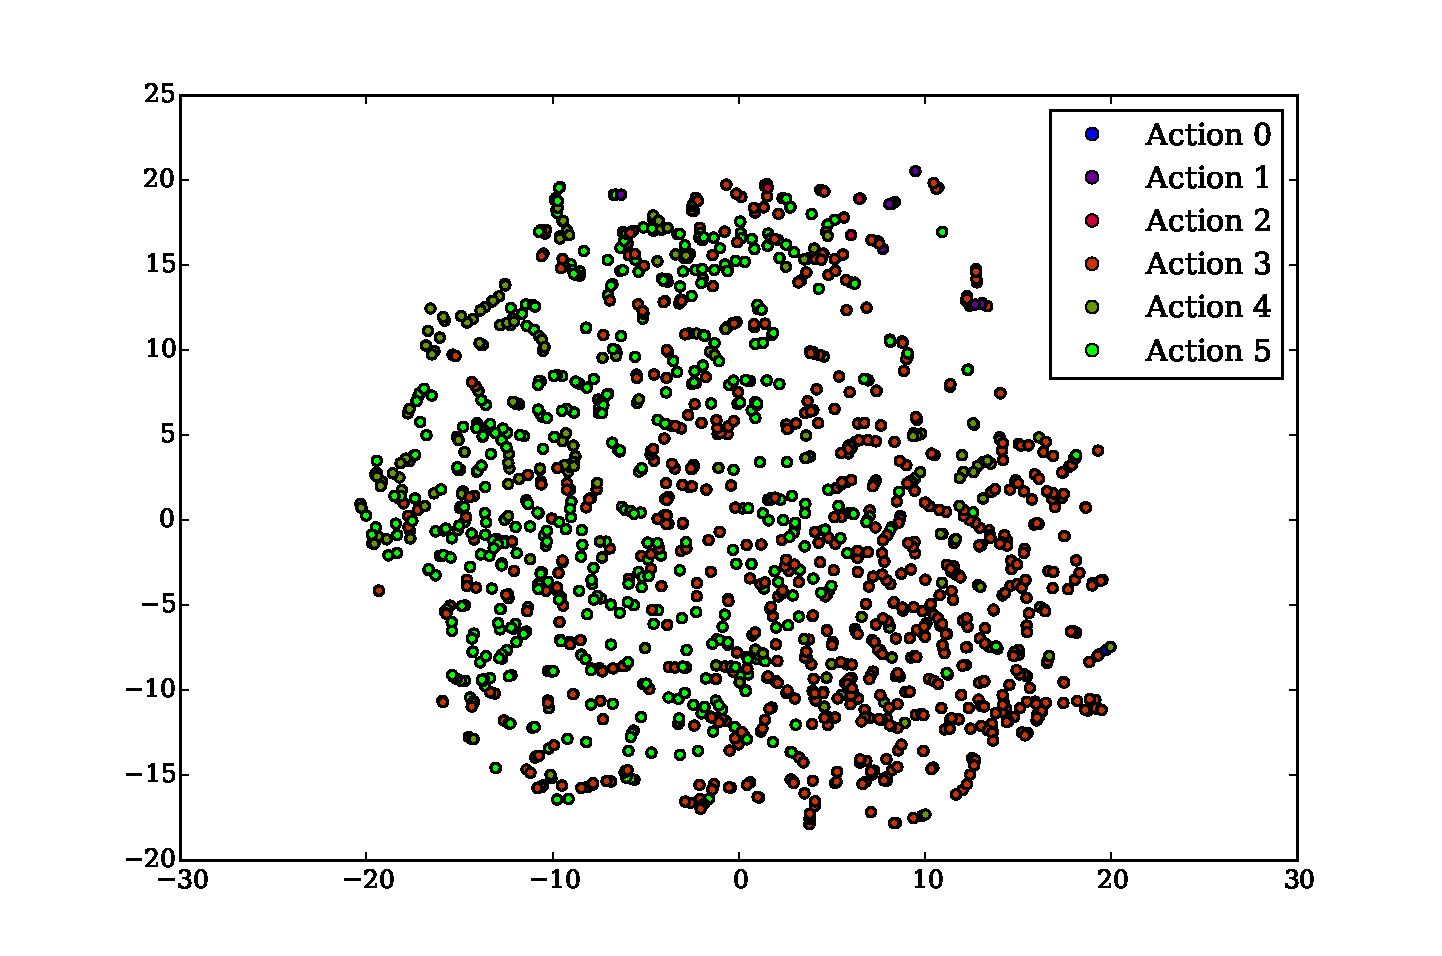
\includegraphics[width=1.5\textwidth]{plots/tsne_breakout_new.pdf}
%  
%  \caption[Fully connected layer's TSNE embedding in Deepmind's network]{The 
% plot shows the TSNE embedding of the last fully connected layer in a network 
% trained for the game of Breakout. The two primary colors--green and brown, 
% respectively, show the two primary actions learned while playing the game of 
% Breakout i.e. left and right respectively and the separation is almost 
% apparent. }
% \label{figure:deepmind}
% \end{figure}
% 
% 
% An extension of this work by \citet*{guo2014deep} 
% improved the results a bit on some games that required extensive planning. They 
% used a Monte-Carlo tree search based player to simulate trajectories, before 
% using the generated state-action-value instances to train a CNN based 
% regression model. The method proved to make a fruitful integration of a 
% planning agent and the RL agent in a way similar to the one discussed 
% in section~\ref{section:RL}.\\ 
% 
% Along with the TSNE embedding in figure~\ref{figure:deepmind}, builds our 
% intuition that the subspace that the convolutional neural network embeds the 
% state representations (i.e. the game screens) in Breakout on the basis of the 
% most favorable action for that state. We will see that 
% regardless of the task specification i.e. either we choose Q-learning (e.g. in 
% \citet{deepmind_nips}) or we choose a regression or classification task (e.g. 
% in \citet{guo2014deep}), we are almost asking the network to embed the states 
% effectively to select the best action.\\
% 
% This is the major motivation to our method of learning the evaluation 
% function for chess boards (state) based on the final outcome of the games, 
% which we describe in the next chapter.
% 	%% Creator: Matplotlib, PGF backend
%%
%% To include the figure in your LaTeX document, write
%%   \input{<filename>.pgf}
%%
%% Make sure the required packages are loaded in your preamble
%%   \usepackage{pgf}
%%
%% Figures using additional raster images can only be included by \input if
%% they are in the same directory as the main LaTeX file. For loading figures
%% from other directories you can use the `import` package
%%   \usepackage{import}
%% and then include the figures with
%%   \import{<path to file>}{<filename>.pgf}
%%
%% Matplotlib used the following preamble
%%   \usepackage{fontspec}
%%   \setmainfont{DejaVu Serif}
%%   \setsansfont{DejaVu Sans}
%%   \setmonofont{DejaVu Sans Mono}
%%
\begingroup%
\makeatletter%
\begin{pgfpicture}%
\pgfpathrectangle{\pgfpointorigin}{\pgfqpoint{8.000000in}{6.000000in}}%
\pgfusepath{use as bounding box, clip}%
\begin{pgfscope}%
\pgfsetbuttcap%
\pgfsetmiterjoin%
\definecolor{currentfill}{rgb}{1.000000,1.000000,1.000000}%
\pgfsetfillcolor{currentfill}%
\pgfsetlinewidth{0.000000pt}%
\definecolor{currentstroke}{rgb}{1.000000,1.000000,1.000000}%
\pgfsetstrokecolor{currentstroke}%
\pgfsetdash{}{0pt}%
\pgfpathmoveto{\pgfqpoint{0.000000in}{0.000000in}}%
\pgfpathlineto{\pgfqpoint{8.000000in}{0.000000in}}%
\pgfpathlineto{\pgfqpoint{8.000000in}{6.000000in}}%
\pgfpathlineto{\pgfqpoint{0.000000in}{6.000000in}}%
\pgfpathclose%
\pgfusepath{fill}%
\end{pgfscope}%
\begin{pgfscope}%
\pgfsetbuttcap%
\pgfsetmiterjoin%
\definecolor{currentfill}{rgb}{1.000000,1.000000,1.000000}%
\pgfsetfillcolor{currentfill}%
\pgfsetlinewidth{0.000000pt}%
\definecolor{currentstroke}{rgb}{0.000000,0.000000,0.000000}%
\pgfsetstrokecolor{currentstroke}%
\pgfsetstrokeopacity{0.000000}%
\pgfsetdash{}{0pt}%
\pgfpathmoveto{\pgfqpoint{1.000000in}{0.600000in}}%
\pgfpathlineto{\pgfqpoint{7.200000in}{0.600000in}}%
\pgfpathlineto{\pgfqpoint{7.200000in}{5.400000in}}%
\pgfpathlineto{\pgfqpoint{1.000000in}{5.400000in}}%
\pgfpathclose%
\pgfusepath{fill}%
\end{pgfscope}%
\begin{pgfscope}%
\pgfpathrectangle{\pgfqpoint{1.000000in}{0.600000in}}{\pgfqpoint{6.200000in}{4.800000in}} %
\pgfusepath{clip}%
\pgfsetbuttcap%
\pgfsetmiterjoin%
\definecolor{currentfill}{rgb}{0.827451,0.827451,0.827451}%
\pgfsetfillcolor{currentfill}%
\pgfsetlinewidth{1.003750pt}%
\definecolor{currentstroke}{rgb}{0.000000,0.000000,0.000000}%
\pgfsetstrokecolor{currentstroke}%
\pgfsetdash{}{0pt}%
\pgfpathmoveto{\pgfqpoint{1.000000in}{0.600000in}}%
\pgfpathlineto{\pgfqpoint{1.258333in}{0.600000in}}%
\pgfpathlineto{\pgfqpoint{1.258333in}{5.180894in}}%
\pgfpathlineto{\pgfqpoint{1.000000in}{5.180894in}}%
\pgfpathlineto{\pgfqpoint{1.000000in}{0.600000in}}%
\pgfusepath{stroke,fill}%
\end{pgfscope}%
\begin{pgfscope}%
\pgfpathrectangle{\pgfqpoint{1.000000in}{0.600000in}}{\pgfqpoint{6.200000in}{4.800000in}} %
\pgfusepath{clip}%
\pgfsetbuttcap%
\pgfsetmiterjoin%
\definecolor{currentfill}{rgb}{0.827451,0.827451,0.827451}%
\pgfsetfillcolor{currentfill}%
\pgfsetlinewidth{1.003750pt}%
\definecolor{currentstroke}{rgb}{0.000000,0.000000,0.000000}%
\pgfsetstrokecolor{currentstroke}%
\pgfsetdash{}{0pt}%
\pgfpathmoveto{\pgfqpoint{2.033333in}{0.600000in}}%
\pgfpathlineto{\pgfqpoint{2.291667in}{0.600000in}}%
\pgfpathlineto{\pgfqpoint{2.291667in}{3.479202in}}%
\pgfpathlineto{\pgfqpoint{2.033333in}{3.479202in}}%
\pgfpathlineto{\pgfqpoint{2.033333in}{0.600000in}}%
\pgfusepath{stroke,fill}%
\end{pgfscope}%
\begin{pgfscope}%
\pgfpathrectangle{\pgfqpoint{1.000000in}{0.600000in}}{\pgfqpoint{6.200000in}{4.800000in}} %
\pgfusepath{clip}%
\pgfsetbuttcap%
\pgfsetmiterjoin%
\definecolor{currentfill}{rgb}{0.827451,0.827451,0.827451}%
\pgfsetfillcolor{currentfill}%
\pgfsetlinewidth{1.003750pt}%
\definecolor{currentstroke}{rgb}{0.000000,0.000000,0.000000}%
\pgfsetstrokecolor{currentstroke}%
\pgfsetdash{}{0pt}%
\pgfpathmoveto{\pgfqpoint{3.066667in}{0.600000in}}%
\pgfpathlineto{\pgfqpoint{3.325000in}{0.600000in}}%
\pgfpathlineto{\pgfqpoint{3.325000in}{3.442842in}}%
\pgfpathlineto{\pgfqpoint{3.066667in}{3.442842in}}%
\pgfpathlineto{\pgfqpoint{3.066667in}{0.600000in}}%
\pgfusepath{stroke,fill}%
\end{pgfscope}%
\begin{pgfscope}%
\pgfpathrectangle{\pgfqpoint{1.000000in}{0.600000in}}{\pgfqpoint{6.200000in}{4.800000in}} %
\pgfusepath{clip}%
\pgfsetbuttcap%
\pgfsetmiterjoin%
\definecolor{currentfill}{rgb}{0.827451,0.827451,0.827451}%
\pgfsetfillcolor{currentfill}%
\pgfsetlinewidth{1.003750pt}%
\definecolor{currentstroke}{rgb}{0.000000,0.000000,0.000000}%
\pgfsetstrokecolor{currentstroke}%
\pgfsetdash{}{0pt}%
\pgfpathmoveto{\pgfqpoint{4.100000in}{0.600000in}}%
\pgfpathlineto{\pgfqpoint{4.358333in}{0.600000in}}%
\pgfpathlineto{\pgfqpoint{4.358333in}{3.232154in}}%
\pgfpathlineto{\pgfqpoint{4.100000in}{3.232154in}}%
\pgfpathlineto{\pgfqpoint{4.100000in}{0.600000in}}%
\pgfusepath{stroke,fill}%
\end{pgfscope}%
\begin{pgfscope}%
\pgfpathrectangle{\pgfqpoint{1.000000in}{0.600000in}}{\pgfqpoint{6.200000in}{4.800000in}} %
\pgfusepath{clip}%
\pgfsetbuttcap%
\pgfsetmiterjoin%
\definecolor{currentfill}{rgb}{0.827451,0.827451,0.827451}%
\pgfsetfillcolor{currentfill}%
\pgfsetlinewidth{1.003750pt}%
\definecolor{currentstroke}{rgb}{0.000000,0.000000,0.000000}%
\pgfsetstrokecolor{currentstroke}%
\pgfsetdash{}{0pt}%
\pgfpathmoveto{\pgfqpoint{5.133333in}{0.600000in}}%
\pgfpathlineto{\pgfqpoint{5.391667in}{0.600000in}}%
\pgfpathlineto{\pgfqpoint{5.391667in}{2.688066in}}%
\pgfpathlineto{\pgfqpoint{5.133333in}{2.688066in}}%
\pgfpathlineto{\pgfqpoint{5.133333in}{0.600000in}}%
\pgfusepath{stroke,fill}%
\end{pgfscope}%
\begin{pgfscope}%
\pgfpathrectangle{\pgfqpoint{1.000000in}{0.600000in}}{\pgfqpoint{6.200000in}{4.800000in}} %
\pgfusepath{clip}%
\pgfsetbuttcap%
\pgfsetmiterjoin%
\definecolor{currentfill}{rgb}{0.827451,0.827451,0.827451}%
\pgfsetfillcolor{currentfill}%
\pgfsetlinewidth{1.003750pt}%
\definecolor{currentstroke}{rgb}{0.000000,0.000000,0.000000}%
\pgfsetstrokecolor{currentstroke}%
\pgfsetdash{}{0pt}%
\pgfpathmoveto{\pgfqpoint{6.166667in}{0.600000in}}%
\pgfpathlineto{\pgfqpoint{6.425000in}{0.600000in}}%
\pgfpathlineto{\pgfqpoint{6.425000in}{2.962474in}}%
\pgfpathlineto{\pgfqpoint{6.166667in}{2.962474in}}%
\pgfpathlineto{\pgfqpoint{6.166667in}{0.600000in}}%
\pgfusepath{stroke,fill}%
\end{pgfscope}%
\begin{pgfscope}%
\pgfpathrectangle{\pgfqpoint{1.000000in}{0.600000in}}{\pgfqpoint{6.200000in}{4.800000in}} %
\pgfusepath{clip}%
\pgfsetbuttcap%
\pgfsetmiterjoin%
\definecolor{currentfill}{rgb}{0.117647,0.564706,1.000000}%
\pgfsetfillcolor{currentfill}%
\pgfsetlinewidth{1.003750pt}%
\definecolor{currentstroke}{rgb}{0.000000,0.000000,0.000000}%
\pgfsetstrokecolor{currentstroke}%
\pgfsetdash{}{0pt}%
\pgfpathmoveto{\pgfqpoint{1.258333in}{0.600000in}}%
\pgfpathlineto{\pgfqpoint{1.516667in}{0.600000in}}%
\pgfpathlineto{\pgfqpoint{1.516667in}{5.381416in}}%
\pgfpathlineto{\pgfqpoint{1.258333in}{5.381416in}}%
\pgfpathlineto{\pgfqpoint{1.258333in}{0.600000in}}%
\pgfusepath{stroke,fill}%
\end{pgfscope}%
\begin{pgfscope}%
\pgfpathrectangle{\pgfqpoint{1.000000in}{0.600000in}}{\pgfqpoint{6.200000in}{4.800000in}} %
\pgfusepath{clip}%
\pgfsetbuttcap%
\pgfsetmiterjoin%
\definecolor{currentfill}{rgb}{0.117647,0.564706,1.000000}%
\pgfsetfillcolor{currentfill}%
\pgfsetlinewidth{1.003750pt}%
\definecolor{currentstroke}{rgb}{0.000000,0.000000,0.000000}%
\pgfsetstrokecolor{currentstroke}%
\pgfsetdash{}{0pt}%
\pgfpathmoveto{\pgfqpoint{2.291667in}{0.600000in}}%
\pgfpathlineto{\pgfqpoint{2.550000in}{0.600000in}}%
\pgfpathlineto{\pgfqpoint{2.550000in}{5.009714in}}%
\pgfpathlineto{\pgfqpoint{2.291667in}{5.009714in}}%
\pgfpathlineto{\pgfqpoint{2.291667in}{0.600000in}}%
\pgfusepath{stroke,fill}%
\end{pgfscope}%
\begin{pgfscope}%
\pgfpathrectangle{\pgfqpoint{1.000000in}{0.600000in}}{\pgfqpoint{6.200000in}{4.800000in}} %
\pgfusepath{clip}%
\pgfsetbuttcap%
\pgfsetmiterjoin%
\definecolor{currentfill}{rgb}{0.117647,0.564706,1.000000}%
\pgfsetfillcolor{currentfill}%
\pgfsetlinewidth{1.003750pt}%
\definecolor{currentstroke}{rgb}{0.000000,0.000000,0.000000}%
\pgfsetstrokecolor{currentstroke}%
\pgfsetdash{}{0pt}%
\pgfpathmoveto{\pgfqpoint{3.325000in}{0.600000in}}%
\pgfpathlineto{\pgfqpoint{3.583333in}{0.600000in}}%
\pgfpathlineto{\pgfqpoint{3.583333in}{3.555010in}}%
\pgfpathlineto{\pgfqpoint{3.325000in}{3.555010in}}%
\pgfpathlineto{\pgfqpoint{3.325000in}{0.600000in}}%
\pgfusepath{stroke,fill}%
\end{pgfscope}%
\begin{pgfscope}%
\pgfpathrectangle{\pgfqpoint{1.000000in}{0.600000in}}{\pgfqpoint{6.200000in}{4.800000in}} %
\pgfusepath{clip}%
\pgfsetbuttcap%
\pgfsetmiterjoin%
\definecolor{currentfill}{rgb}{0.117647,0.564706,1.000000}%
\pgfsetfillcolor{currentfill}%
\pgfsetlinewidth{1.003750pt}%
\definecolor{currentstroke}{rgb}{0.000000,0.000000,0.000000}%
\pgfsetstrokecolor{currentstroke}%
\pgfsetdash{}{0pt}%
\pgfpathmoveto{\pgfqpoint{4.358333in}{0.600000in}}%
\pgfpathlineto{\pgfqpoint{4.616667in}{0.600000in}}%
\pgfpathlineto{\pgfqpoint{4.616667in}{3.841903in}}%
\pgfpathlineto{\pgfqpoint{4.358333in}{3.841903in}}%
\pgfpathlineto{\pgfqpoint{4.358333in}{0.600000in}}%
\pgfusepath{stroke,fill}%
\end{pgfscope}%
\begin{pgfscope}%
\pgfpathrectangle{\pgfqpoint{1.000000in}{0.600000in}}{\pgfqpoint{6.200000in}{4.800000in}} %
\pgfusepath{clip}%
\pgfsetbuttcap%
\pgfsetmiterjoin%
\definecolor{currentfill}{rgb}{0.117647,0.564706,1.000000}%
\pgfsetfillcolor{currentfill}%
\pgfsetlinewidth{1.003750pt}%
\definecolor{currentstroke}{rgb}{0.000000,0.000000,0.000000}%
\pgfsetstrokecolor{currentstroke}%
\pgfsetdash{}{0pt}%
\pgfpathmoveto{\pgfqpoint{5.391667in}{0.600000in}}%
\pgfpathlineto{\pgfqpoint{5.650000in}{0.600000in}}%
\pgfpathlineto{\pgfqpoint{5.650000in}{3.505016in}}%
\pgfpathlineto{\pgfqpoint{5.391667in}{3.505016in}}%
\pgfpathlineto{\pgfqpoint{5.391667in}{0.600000in}}%
\pgfusepath{stroke,fill}%
\end{pgfscope}%
\begin{pgfscope}%
\pgfpathrectangle{\pgfqpoint{1.000000in}{0.600000in}}{\pgfqpoint{6.200000in}{4.800000in}} %
\pgfusepath{clip}%
\pgfsetbuttcap%
\pgfsetmiterjoin%
\definecolor{currentfill}{rgb}{0.117647,0.564706,1.000000}%
\pgfsetfillcolor{currentfill}%
\pgfsetlinewidth{1.003750pt}%
\definecolor{currentstroke}{rgb}{0.000000,0.000000,0.000000}%
\pgfsetstrokecolor{currentstroke}%
\pgfsetdash{}{0pt}%
\pgfpathmoveto{\pgfqpoint{6.425000in}{0.600000in}}%
\pgfpathlineto{\pgfqpoint{6.683333in}{0.600000in}}%
\pgfpathlineto{\pgfqpoint{6.683333in}{4.474843in}}%
\pgfpathlineto{\pgfqpoint{6.425000in}{4.474843in}}%
\pgfpathlineto{\pgfqpoint{6.425000in}{0.600000in}}%
\pgfusepath{stroke,fill}%
\end{pgfscope}%
\begin{pgfscope}%
\pgfsetrectcap%
\pgfsetmiterjoin%
\pgfsetlinewidth{1.003750pt}%
\definecolor{currentstroke}{rgb}{0.000000,0.000000,0.000000}%
\pgfsetstrokecolor{currentstroke}%
\pgfsetdash{}{0pt}%
\pgfpathmoveto{\pgfqpoint{1.000000in}{5.400000in}}%
\pgfpathlineto{\pgfqpoint{7.200000in}{5.400000in}}%
\pgfusepath{stroke}%
\end{pgfscope}%
\begin{pgfscope}%
\pgfsetrectcap%
\pgfsetmiterjoin%
\pgfsetlinewidth{1.003750pt}%
\definecolor{currentstroke}{rgb}{0.000000,0.000000,0.000000}%
\pgfsetstrokecolor{currentstroke}%
\pgfsetdash{}{0pt}%
\pgfpathmoveto{\pgfqpoint{7.200000in}{0.600000in}}%
\pgfpathlineto{\pgfqpoint{7.200000in}{5.400000in}}%
\pgfusepath{stroke}%
\end{pgfscope}%
\begin{pgfscope}%
\pgfsetrectcap%
\pgfsetmiterjoin%
\pgfsetlinewidth{1.003750pt}%
\definecolor{currentstroke}{rgb}{0.000000,0.000000,0.000000}%
\pgfsetstrokecolor{currentstroke}%
\pgfsetdash{}{0pt}%
\pgfpathmoveto{\pgfqpoint{1.000000in}{0.600000in}}%
\pgfpathlineto{\pgfqpoint{7.200000in}{0.600000in}}%
\pgfusepath{stroke}%
\end{pgfscope}%
\begin{pgfscope}%
\pgfsetrectcap%
\pgfsetmiterjoin%
\pgfsetlinewidth{1.003750pt}%
\definecolor{currentstroke}{rgb}{0.000000,0.000000,0.000000}%
\pgfsetstrokecolor{currentstroke}%
\pgfsetdash{}{0pt}%
\pgfpathmoveto{\pgfqpoint{1.000000in}{0.600000in}}%
\pgfpathlineto{\pgfqpoint{1.000000in}{5.400000in}}%
\pgfusepath{stroke}%
\end{pgfscope}%
\begin{pgfscope}%
\pgfsetbuttcap%
\pgfsetroundjoin%
\definecolor{currentfill}{rgb}{0.000000,0.000000,0.000000}%
\pgfsetfillcolor{currentfill}%
\pgfsetlinewidth{0.501875pt}%
\definecolor{currentstroke}{rgb}{0.000000,0.000000,0.000000}%
\pgfsetstrokecolor{currentstroke}%
\pgfsetdash{}{0pt}%
\pgfsys@defobject{currentmarker}{\pgfqpoint{0.000000in}{0.000000in}}{\pgfqpoint{0.000000in}{0.055556in}}{%
\pgfpathmoveto{\pgfqpoint{0.000000in}{0.000000in}}%
\pgfpathlineto{\pgfqpoint{0.000000in}{0.055556in}}%
\pgfusepath{stroke,fill}%
}%
\begin{pgfscope}%
\pgfsys@transformshift{1.258333in}{0.600000in}%
\pgfsys@useobject{currentmarker}{}%
\end{pgfscope}%
\end{pgfscope}%
\begin{pgfscope}%
\pgfsetbuttcap%
\pgfsetroundjoin%
\definecolor{currentfill}{rgb}{0.000000,0.000000,0.000000}%
\pgfsetfillcolor{currentfill}%
\pgfsetlinewidth{0.501875pt}%
\definecolor{currentstroke}{rgb}{0.000000,0.000000,0.000000}%
\pgfsetstrokecolor{currentstroke}%
\pgfsetdash{}{0pt}%
\pgfsys@defobject{currentmarker}{\pgfqpoint{0.000000in}{-0.055556in}}{\pgfqpoint{0.000000in}{0.000000in}}{%
\pgfpathmoveto{\pgfqpoint{0.000000in}{0.000000in}}%
\pgfpathlineto{\pgfqpoint{0.000000in}{-0.055556in}}%
\pgfusepath{stroke,fill}%
}%
\begin{pgfscope}%
\pgfsys@transformshift{1.258333in}{5.400000in}%
\pgfsys@useobject{currentmarker}{}%
\end{pgfscope}%
\end{pgfscope}%
\begin{pgfscope}%
\pgftext[x=1.258333in,y=0.544444in,,top]{\rmfamily\fontsize{12.000000}{14.400000}\selectfont Pawn}%
\end{pgfscope}%
\begin{pgfscope}%
\pgfsetbuttcap%
\pgfsetroundjoin%
\definecolor{currentfill}{rgb}{0.000000,0.000000,0.000000}%
\pgfsetfillcolor{currentfill}%
\pgfsetlinewidth{0.501875pt}%
\definecolor{currentstroke}{rgb}{0.000000,0.000000,0.000000}%
\pgfsetstrokecolor{currentstroke}%
\pgfsetdash{}{0pt}%
\pgfsys@defobject{currentmarker}{\pgfqpoint{0.000000in}{0.000000in}}{\pgfqpoint{0.000000in}{0.055556in}}{%
\pgfpathmoveto{\pgfqpoint{0.000000in}{0.000000in}}%
\pgfpathlineto{\pgfqpoint{0.000000in}{0.055556in}}%
\pgfusepath{stroke,fill}%
}%
\begin{pgfscope}%
\pgfsys@transformshift{2.291667in}{0.600000in}%
\pgfsys@useobject{currentmarker}{}%
\end{pgfscope}%
\end{pgfscope}%
\begin{pgfscope}%
\pgfsetbuttcap%
\pgfsetroundjoin%
\definecolor{currentfill}{rgb}{0.000000,0.000000,0.000000}%
\pgfsetfillcolor{currentfill}%
\pgfsetlinewidth{0.501875pt}%
\definecolor{currentstroke}{rgb}{0.000000,0.000000,0.000000}%
\pgfsetstrokecolor{currentstroke}%
\pgfsetdash{}{0pt}%
\pgfsys@defobject{currentmarker}{\pgfqpoint{0.000000in}{-0.055556in}}{\pgfqpoint{0.000000in}{0.000000in}}{%
\pgfpathmoveto{\pgfqpoint{0.000000in}{0.000000in}}%
\pgfpathlineto{\pgfqpoint{0.000000in}{-0.055556in}}%
\pgfusepath{stroke,fill}%
}%
\begin{pgfscope}%
\pgfsys@transformshift{2.291667in}{5.400000in}%
\pgfsys@useobject{currentmarker}{}%
\end{pgfscope}%
\end{pgfscope}%
\begin{pgfscope}%
\pgftext[x=2.291667in,y=0.544444in,,top]{\rmfamily\fontsize{12.000000}{14.400000}\selectfont Rook}%
\end{pgfscope}%
\begin{pgfscope}%
\pgfsetbuttcap%
\pgfsetroundjoin%
\definecolor{currentfill}{rgb}{0.000000,0.000000,0.000000}%
\pgfsetfillcolor{currentfill}%
\pgfsetlinewidth{0.501875pt}%
\definecolor{currentstroke}{rgb}{0.000000,0.000000,0.000000}%
\pgfsetstrokecolor{currentstroke}%
\pgfsetdash{}{0pt}%
\pgfsys@defobject{currentmarker}{\pgfqpoint{0.000000in}{0.000000in}}{\pgfqpoint{0.000000in}{0.055556in}}{%
\pgfpathmoveto{\pgfqpoint{0.000000in}{0.000000in}}%
\pgfpathlineto{\pgfqpoint{0.000000in}{0.055556in}}%
\pgfusepath{stroke,fill}%
}%
\begin{pgfscope}%
\pgfsys@transformshift{3.325000in}{0.600000in}%
\pgfsys@useobject{currentmarker}{}%
\end{pgfscope}%
\end{pgfscope}%
\begin{pgfscope}%
\pgfsetbuttcap%
\pgfsetroundjoin%
\definecolor{currentfill}{rgb}{0.000000,0.000000,0.000000}%
\pgfsetfillcolor{currentfill}%
\pgfsetlinewidth{0.501875pt}%
\definecolor{currentstroke}{rgb}{0.000000,0.000000,0.000000}%
\pgfsetstrokecolor{currentstroke}%
\pgfsetdash{}{0pt}%
\pgfsys@defobject{currentmarker}{\pgfqpoint{0.000000in}{-0.055556in}}{\pgfqpoint{0.000000in}{0.000000in}}{%
\pgfpathmoveto{\pgfqpoint{0.000000in}{0.000000in}}%
\pgfpathlineto{\pgfqpoint{0.000000in}{-0.055556in}}%
\pgfusepath{stroke,fill}%
}%
\begin{pgfscope}%
\pgfsys@transformshift{3.325000in}{5.400000in}%
\pgfsys@useobject{currentmarker}{}%
\end{pgfscope}%
\end{pgfscope}%
\begin{pgfscope}%
\pgftext[x=3.325000in,y=0.544444in,,top]{\rmfamily\fontsize{12.000000}{14.400000}\selectfont Knight}%
\end{pgfscope}%
\begin{pgfscope}%
\pgfsetbuttcap%
\pgfsetroundjoin%
\definecolor{currentfill}{rgb}{0.000000,0.000000,0.000000}%
\pgfsetfillcolor{currentfill}%
\pgfsetlinewidth{0.501875pt}%
\definecolor{currentstroke}{rgb}{0.000000,0.000000,0.000000}%
\pgfsetstrokecolor{currentstroke}%
\pgfsetdash{}{0pt}%
\pgfsys@defobject{currentmarker}{\pgfqpoint{0.000000in}{0.000000in}}{\pgfqpoint{0.000000in}{0.055556in}}{%
\pgfpathmoveto{\pgfqpoint{0.000000in}{0.000000in}}%
\pgfpathlineto{\pgfqpoint{0.000000in}{0.055556in}}%
\pgfusepath{stroke,fill}%
}%
\begin{pgfscope}%
\pgfsys@transformshift{4.358333in}{0.600000in}%
\pgfsys@useobject{currentmarker}{}%
\end{pgfscope}%
\end{pgfscope}%
\begin{pgfscope}%
\pgfsetbuttcap%
\pgfsetroundjoin%
\definecolor{currentfill}{rgb}{0.000000,0.000000,0.000000}%
\pgfsetfillcolor{currentfill}%
\pgfsetlinewidth{0.501875pt}%
\definecolor{currentstroke}{rgb}{0.000000,0.000000,0.000000}%
\pgfsetstrokecolor{currentstroke}%
\pgfsetdash{}{0pt}%
\pgfsys@defobject{currentmarker}{\pgfqpoint{0.000000in}{-0.055556in}}{\pgfqpoint{0.000000in}{0.000000in}}{%
\pgfpathmoveto{\pgfqpoint{0.000000in}{0.000000in}}%
\pgfpathlineto{\pgfqpoint{0.000000in}{-0.055556in}}%
\pgfusepath{stroke,fill}%
}%
\begin{pgfscope}%
\pgfsys@transformshift{4.358333in}{5.400000in}%
\pgfsys@useobject{currentmarker}{}%
\end{pgfscope}%
\end{pgfscope}%
\begin{pgfscope}%
\pgftext[x=4.358333in,y=0.544444in,,top]{\rmfamily\fontsize{12.000000}{14.400000}\selectfont Bishop}%
\end{pgfscope}%
\begin{pgfscope}%
\pgfsetbuttcap%
\pgfsetroundjoin%
\definecolor{currentfill}{rgb}{0.000000,0.000000,0.000000}%
\pgfsetfillcolor{currentfill}%
\pgfsetlinewidth{0.501875pt}%
\definecolor{currentstroke}{rgb}{0.000000,0.000000,0.000000}%
\pgfsetstrokecolor{currentstroke}%
\pgfsetdash{}{0pt}%
\pgfsys@defobject{currentmarker}{\pgfqpoint{0.000000in}{0.000000in}}{\pgfqpoint{0.000000in}{0.055556in}}{%
\pgfpathmoveto{\pgfqpoint{0.000000in}{0.000000in}}%
\pgfpathlineto{\pgfqpoint{0.000000in}{0.055556in}}%
\pgfusepath{stroke,fill}%
}%
\begin{pgfscope}%
\pgfsys@transformshift{5.391667in}{0.600000in}%
\pgfsys@useobject{currentmarker}{}%
\end{pgfscope}%
\end{pgfscope}%
\begin{pgfscope}%
\pgfsetbuttcap%
\pgfsetroundjoin%
\definecolor{currentfill}{rgb}{0.000000,0.000000,0.000000}%
\pgfsetfillcolor{currentfill}%
\pgfsetlinewidth{0.501875pt}%
\definecolor{currentstroke}{rgb}{0.000000,0.000000,0.000000}%
\pgfsetstrokecolor{currentstroke}%
\pgfsetdash{}{0pt}%
\pgfsys@defobject{currentmarker}{\pgfqpoint{0.000000in}{-0.055556in}}{\pgfqpoint{0.000000in}{0.000000in}}{%
\pgfpathmoveto{\pgfqpoint{0.000000in}{0.000000in}}%
\pgfpathlineto{\pgfqpoint{0.000000in}{-0.055556in}}%
\pgfusepath{stroke,fill}%
}%
\begin{pgfscope}%
\pgfsys@transformshift{5.391667in}{5.400000in}%
\pgfsys@useobject{currentmarker}{}%
\end{pgfscope}%
\end{pgfscope}%
\begin{pgfscope}%
\pgftext[x=5.391667in,y=0.544444in,,top]{\rmfamily\fontsize{12.000000}{14.400000}\selectfont Queen}%
\end{pgfscope}%
\begin{pgfscope}%
\pgfsetbuttcap%
\pgfsetroundjoin%
\definecolor{currentfill}{rgb}{0.000000,0.000000,0.000000}%
\pgfsetfillcolor{currentfill}%
\pgfsetlinewidth{0.501875pt}%
\definecolor{currentstroke}{rgb}{0.000000,0.000000,0.000000}%
\pgfsetstrokecolor{currentstroke}%
\pgfsetdash{}{0pt}%
\pgfsys@defobject{currentmarker}{\pgfqpoint{0.000000in}{0.000000in}}{\pgfqpoint{0.000000in}{0.055556in}}{%
\pgfpathmoveto{\pgfqpoint{0.000000in}{0.000000in}}%
\pgfpathlineto{\pgfqpoint{0.000000in}{0.055556in}}%
\pgfusepath{stroke,fill}%
}%
\begin{pgfscope}%
\pgfsys@transformshift{6.425000in}{0.600000in}%
\pgfsys@useobject{currentmarker}{}%
\end{pgfscope}%
\end{pgfscope}%
\begin{pgfscope}%
\pgfsetbuttcap%
\pgfsetroundjoin%
\definecolor{currentfill}{rgb}{0.000000,0.000000,0.000000}%
\pgfsetfillcolor{currentfill}%
\pgfsetlinewidth{0.501875pt}%
\definecolor{currentstroke}{rgb}{0.000000,0.000000,0.000000}%
\pgfsetstrokecolor{currentstroke}%
\pgfsetdash{}{0pt}%
\pgfsys@defobject{currentmarker}{\pgfqpoint{0.000000in}{-0.055556in}}{\pgfqpoint{0.000000in}{0.000000in}}{%
\pgfpathmoveto{\pgfqpoint{0.000000in}{0.000000in}}%
\pgfpathlineto{\pgfqpoint{0.000000in}{-0.055556in}}%
\pgfusepath{stroke,fill}%
}%
\begin{pgfscope}%
\pgfsys@transformshift{6.425000in}{5.400000in}%
\pgfsys@useobject{currentmarker}{}%
\end{pgfscope}%
\end{pgfscope}%
\begin{pgfscope}%
\pgftext[x=6.425000in,y=0.544444in,,top]{\rmfamily\fontsize{12.000000}{14.400000}\selectfont King}%
\end{pgfscope}%
\begin{pgfscope}%
\pgftext[x=4.100000in,y=0.311345in,,top]{\rmfamily\fontsize{12.000000}{14.400000}\selectfont Piece types}%
\end{pgfscope}%
\begin{pgfscope}%
\pgfsetbuttcap%
\pgfsetroundjoin%
\definecolor{currentfill}{rgb}{0.000000,0.000000,0.000000}%
\pgfsetfillcolor{currentfill}%
\pgfsetlinewidth{0.501875pt}%
\definecolor{currentstroke}{rgb}{0.000000,0.000000,0.000000}%
\pgfsetstrokecolor{currentstroke}%
\pgfsetdash{}{0pt}%
\pgfsys@defobject{currentmarker}{\pgfqpoint{0.000000in}{0.000000in}}{\pgfqpoint{0.055556in}{0.000000in}}{%
\pgfpathmoveto{\pgfqpoint{0.000000in}{0.000000in}}%
\pgfpathlineto{\pgfqpoint{0.055556in}{0.000000in}}%
\pgfusepath{stroke,fill}%
}%
\begin{pgfscope}%
\pgfsys@transformshift{1.000000in}{0.600000in}%
\pgfsys@useobject{currentmarker}{}%
\end{pgfscope}%
\end{pgfscope}%
\begin{pgfscope}%
\pgfsetbuttcap%
\pgfsetroundjoin%
\definecolor{currentfill}{rgb}{0.000000,0.000000,0.000000}%
\pgfsetfillcolor{currentfill}%
\pgfsetlinewidth{0.501875pt}%
\definecolor{currentstroke}{rgb}{0.000000,0.000000,0.000000}%
\pgfsetstrokecolor{currentstroke}%
\pgfsetdash{}{0pt}%
\pgfsys@defobject{currentmarker}{\pgfqpoint{-0.055556in}{0.000000in}}{\pgfqpoint{0.000000in}{0.000000in}}{%
\pgfpathmoveto{\pgfqpoint{0.000000in}{0.000000in}}%
\pgfpathlineto{\pgfqpoint{-0.055556in}{0.000000in}}%
\pgfusepath{stroke,fill}%
}%
\begin{pgfscope}%
\pgfsys@transformshift{7.200000in}{0.600000in}%
\pgfsys@useobject{currentmarker}{}%
\end{pgfscope}%
\end{pgfscope}%
\begin{pgfscope}%
\pgftext[x=0.944444in,y=0.600000in,right,]{\rmfamily\fontsize{12.000000}{14.400000}\selectfont 0}%
\end{pgfscope}%
\begin{pgfscope}%
\pgfsetbuttcap%
\pgfsetroundjoin%
\definecolor{currentfill}{rgb}{0.000000,0.000000,0.000000}%
\pgfsetfillcolor{currentfill}%
\pgfsetlinewidth{0.501875pt}%
\definecolor{currentstroke}{rgb}{0.000000,0.000000,0.000000}%
\pgfsetstrokecolor{currentstroke}%
\pgfsetdash{}{0pt}%
\pgfsys@defobject{currentmarker}{\pgfqpoint{0.000000in}{0.000000in}}{\pgfqpoint{0.055556in}{0.000000in}}{%
\pgfpathmoveto{\pgfqpoint{0.000000in}{0.000000in}}%
\pgfpathlineto{\pgfqpoint{0.055556in}{0.000000in}}%
\pgfusepath{stroke,fill}%
}%
\begin{pgfscope}%
\pgfsys@transformshift{1.000000in}{1.133333in}%
\pgfsys@useobject{currentmarker}{}%
\end{pgfscope}%
\end{pgfscope}%
\begin{pgfscope}%
\pgfsetbuttcap%
\pgfsetroundjoin%
\definecolor{currentfill}{rgb}{0.000000,0.000000,0.000000}%
\pgfsetfillcolor{currentfill}%
\pgfsetlinewidth{0.501875pt}%
\definecolor{currentstroke}{rgb}{0.000000,0.000000,0.000000}%
\pgfsetstrokecolor{currentstroke}%
\pgfsetdash{}{0pt}%
\pgfsys@defobject{currentmarker}{\pgfqpoint{-0.055556in}{0.000000in}}{\pgfqpoint{0.000000in}{0.000000in}}{%
\pgfpathmoveto{\pgfqpoint{0.000000in}{0.000000in}}%
\pgfpathlineto{\pgfqpoint{-0.055556in}{0.000000in}}%
\pgfusepath{stroke,fill}%
}%
\begin{pgfscope}%
\pgfsys@transformshift{7.200000in}{1.133333in}%
\pgfsys@useobject{currentmarker}{}%
\end{pgfscope}%
\end{pgfscope}%
\begin{pgfscope}%
\pgftext[x=0.944444in,y=1.133333in,right,]{\rmfamily\fontsize{12.000000}{14.400000}\selectfont 1000000}%
\end{pgfscope}%
\begin{pgfscope}%
\pgfsetbuttcap%
\pgfsetroundjoin%
\definecolor{currentfill}{rgb}{0.000000,0.000000,0.000000}%
\pgfsetfillcolor{currentfill}%
\pgfsetlinewidth{0.501875pt}%
\definecolor{currentstroke}{rgb}{0.000000,0.000000,0.000000}%
\pgfsetstrokecolor{currentstroke}%
\pgfsetdash{}{0pt}%
\pgfsys@defobject{currentmarker}{\pgfqpoint{0.000000in}{0.000000in}}{\pgfqpoint{0.055556in}{0.000000in}}{%
\pgfpathmoveto{\pgfqpoint{0.000000in}{0.000000in}}%
\pgfpathlineto{\pgfqpoint{0.055556in}{0.000000in}}%
\pgfusepath{stroke,fill}%
}%
\begin{pgfscope}%
\pgfsys@transformshift{1.000000in}{1.666667in}%
\pgfsys@useobject{currentmarker}{}%
\end{pgfscope}%
\end{pgfscope}%
\begin{pgfscope}%
\pgfsetbuttcap%
\pgfsetroundjoin%
\definecolor{currentfill}{rgb}{0.000000,0.000000,0.000000}%
\pgfsetfillcolor{currentfill}%
\pgfsetlinewidth{0.501875pt}%
\definecolor{currentstroke}{rgb}{0.000000,0.000000,0.000000}%
\pgfsetstrokecolor{currentstroke}%
\pgfsetdash{}{0pt}%
\pgfsys@defobject{currentmarker}{\pgfqpoint{-0.055556in}{0.000000in}}{\pgfqpoint{0.000000in}{0.000000in}}{%
\pgfpathmoveto{\pgfqpoint{0.000000in}{0.000000in}}%
\pgfpathlineto{\pgfqpoint{-0.055556in}{0.000000in}}%
\pgfusepath{stroke,fill}%
}%
\begin{pgfscope}%
\pgfsys@transformshift{7.200000in}{1.666667in}%
\pgfsys@useobject{currentmarker}{}%
\end{pgfscope}%
\end{pgfscope}%
\begin{pgfscope}%
\pgftext[x=0.944444in,y=1.666667in,right,]{\rmfamily\fontsize{12.000000}{14.400000}\selectfont 2000000}%
\end{pgfscope}%
\begin{pgfscope}%
\pgfsetbuttcap%
\pgfsetroundjoin%
\definecolor{currentfill}{rgb}{0.000000,0.000000,0.000000}%
\pgfsetfillcolor{currentfill}%
\pgfsetlinewidth{0.501875pt}%
\definecolor{currentstroke}{rgb}{0.000000,0.000000,0.000000}%
\pgfsetstrokecolor{currentstroke}%
\pgfsetdash{}{0pt}%
\pgfsys@defobject{currentmarker}{\pgfqpoint{0.000000in}{0.000000in}}{\pgfqpoint{0.055556in}{0.000000in}}{%
\pgfpathmoveto{\pgfqpoint{0.000000in}{0.000000in}}%
\pgfpathlineto{\pgfqpoint{0.055556in}{0.000000in}}%
\pgfusepath{stroke,fill}%
}%
\begin{pgfscope}%
\pgfsys@transformshift{1.000000in}{2.200000in}%
\pgfsys@useobject{currentmarker}{}%
\end{pgfscope}%
\end{pgfscope}%
\begin{pgfscope}%
\pgfsetbuttcap%
\pgfsetroundjoin%
\definecolor{currentfill}{rgb}{0.000000,0.000000,0.000000}%
\pgfsetfillcolor{currentfill}%
\pgfsetlinewidth{0.501875pt}%
\definecolor{currentstroke}{rgb}{0.000000,0.000000,0.000000}%
\pgfsetstrokecolor{currentstroke}%
\pgfsetdash{}{0pt}%
\pgfsys@defobject{currentmarker}{\pgfqpoint{-0.055556in}{0.000000in}}{\pgfqpoint{0.000000in}{0.000000in}}{%
\pgfpathmoveto{\pgfqpoint{0.000000in}{0.000000in}}%
\pgfpathlineto{\pgfqpoint{-0.055556in}{0.000000in}}%
\pgfusepath{stroke,fill}%
}%
\begin{pgfscope}%
\pgfsys@transformshift{7.200000in}{2.200000in}%
\pgfsys@useobject{currentmarker}{}%
\end{pgfscope}%
\end{pgfscope}%
\begin{pgfscope}%
\pgftext[x=0.944444in,y=2.200000in,right,]{\rmfamily\fontsize{12.000000}{14.400000}\selectfont 3000000}%
\end{pgfscope}%
\begin{pgfscope}%
\pgfsetbuttcap%
\pgfsetroundjoin%
\definecolor{currentfill}{rgb}{0.000000,0.000000,0.000000}%
\pgfsetfillcolor{currentfill}%
\pgfsetlinewidth{0.501875pt}%
\definecolor{currentstroke}{rgb}{0.000000,0.000000,0.000000}%
\pgfsetstrokecolor{currentstroke}%
\pgfsetdash{}{0pt}%
\pgfsys@defobject{currentmarker}{\pgfqpoint{0.000000in}{0.000000in}}{\pgfqpoint{0.055556in}{0.000000in}}{%
\pgfpathmoveto{\pgfqpoint{0.000000in}{0.000000in}}%
\pgfpathlineto{\pgfqpoint{0.055556in}{0.000000in}}%
\pgfusepath{stroke,fill}%
}%
\begin{pgfscope}%
\pgfsys@transformshift{1.000000in}{2.733333in}%
\pgfsys@useobject{currentmarker}{}%
\end{pgfscope}%
\end{pgfscope}%
\begin{pgfscope}%
\pgfsetbuttcap%
\pgfsetroundjoin%
\definecolor{currentfill}{rgb}{0.000000,0.000000,0.000000}%
\pgfsetfillcolor{currentfill}%
\pgfsetlinewidth{0.501875pt}%
\definecolor{currentstroke}{rgb}{0.000000,0.000000,0.000000}%
\pgfsetstrokecolor{currentstroke}%
\pgfsetdash{}{0pt}%
\pgfsys@defobject{currentmarker}{\pgfqpoint{-0.055556in}{0.000000in}}{\pgfqpoint{0.000000in}{0.000000in}}{%
\pgfpathmoveto{\pgfqpoint{0.000000in}{0.000000in}}%
\pgfpathlineto{\pgfqpoint{-0.055556in}{0.000000in}}%
\pgfusepath{stroke,fill}%
}%
\begin{pgfscope}%
\pgfsys@transformshift{7.200000in}{2.733333in}%
\pgfsys@useobject{currentmarker}{}%
\end{pgfscope}%
\end{pgfscope}%
\begin{pgfscope}%
\pgftext[x=0.944444in,y=2.733333in,right,]{\rmfamily\fontsize{12.000000}{14.400000}\selectfont 4000000}%
\end{pgfscope}%
\begin{pgfscope}%
\pgfsetbuttcap%
\pgfsetroundjoin%
\definecolor{currentfill}{rgb}{0.000000,0.000000,0.000000}%
\pgfsetfillcolor{currentfill}%
\pgfsetlinewidth{0.501875pt}%
\definecolor{currentstroke}{rgb}{0.000000,0.000000,0.000000}%
\pgfsetstrokecolor{currentstroke}%
\pgfsetdash{}{0pt}%
\pgfsys@defobject{currentmarker}{\pgfqpoint{0.000000in}{0.000000in}}{\pgfqpoint{0.055556in}{0.000000in}}{%
\pgfpathmoveto{\pgfqpoint{0.000000in}{0.000000in}}%
\pgfpathlineto{\pgfqpoint{0.055556in}{0.000000in}}%
\pgfusepath{stroke,fill}%
}%
\begin{pgfscope}%
\pgfsys@transformshift{1.000000in}{3.266667in}%
\pgfsys@useobject{currentmarker}{}%
\end{pgfscope}%
\end{pgfscope}%
\begin{pgfscope}%
\pgfsetbuttcap%
\pgfsetroundjoin%
\definecolor{currentfill}{rgb}{0.000000,0.000000,0.000000}%
\pgfsetfillcolor{currentfill}%
\pgfsetlinewidth{0.501875pt}%
\definecolor{currentstroke}{rgb}{0.000000,0.000000,0.000000}%
\pgfsetstrokecolor{currentstroke}%
\pgfsetdash{}{0pt}%
\pgfsys@defobject{currentmarker}{\pgfqpoint{-0.055556in}{0.000000in}}{\pgfqpoint{0.000000in}{0.000000in}}{%
\pgfpathmoveto{\pgfqpoint{0.000000in}{0.000000in}}%
\pgfpathlineto{\pgfqpoint{-0.055556in}{0.000000in}}%
\pgfusepath{stroke,fill}%
}%
\begin{pgfscope}%
\pgfsys@transformshift{7.200000in}{3.266667in}%
\pgfsys@useobject{currentmarker}{}%
\end{pgfscope}%
\end{pgfscope}%
\begin{pgfscope}%
\pgftext[x=0.944444in,y=3.266667in,right,]{\rmfamily\fontsize{12.000000}{14.400000}\selectfont 5000000}%
\end{pgfscope}%
\begin{pgfscope}%
\pgfsetbuttcap%
\pgfsetroundjoin%
\definecolor{currentfill}{rgb}{0.000000,0.000000,0.000000}%
\pgfsetfillcolor{currentfill}%
\pgfsetlinewidth{0.501875pt}%
\definecolor{currentstroke}{rgb}{0.000000,0.000000,0.000000}%
\pgfsetstrokecolor{currentstroke}%
\pgfsetdash{}{0pt}%
\pgfsys@defobject{currentmarker}{\pgfqpoint{0.000000in}{0.000000in}}{\pgfqpoint{0.055556in}{0.000000in}}{%
\pgfpathmoveto{\pgfqpoint{0.000000in}{0.000000in}}%
\pgfpathlineto{\pgfqpoint{0.055556in}{0.000000in}}%
\pgfusepath{stroke,fill}%
}%
\begin{pgfscope}%
\pgfsys@transformshift{1.000000in}{3.800000in}%
\pgfsys@useobject{currentmarker}{}%
\end{pgfscope}%
\end{pgfscope}%
\begin{pgfscope}%
\pgfsetbuttcap%
\pgfsetroundjoin%
\definecolor{currentfill}{rgb}{0.000000,0.000000,0.000000}%
\pgfsetfillcolor{currentfill}%
\pgfsetlinewidth{0.501875pt}%
\definecolor{currentstroke}{rgb}{0.000000,0.000000,0.000000}%
\pgfsetstrokecolor{currentstroke}%
\pgfsetdash{}{0pt}%
\pgfsys@defobject{currentmarker}{\pgfqpoint{-0.055556in}{0.000000in}}{\pgfqpoint{0.000000in}{0.000000in}}{%
\pgfpathmoveto{\pgfqpoint{0.000000in}{0.000000in}}%
\pgfpathlineto{\pgfqpoint{-0.055556in}{0.000000in}}%
\pgfusepath{stroke,fill}%
}%
\begin{pgfscope}%
\pgfsys@transformshift{7.200000in}{3.800000in}%
\pgfsys@useobject{currentmarker}{}%
\end{pgfscope}%
\end{pgfscope}%
\begin{pgfscope}%
\pgftext[x=0.944444in,y=3.800000in,right,]{\rmfamily\fontsize{12.000000}{14.400000}\selectfont 6000000}%
\end{pgfscope}%
\begin{pgfscope}%
\pgfsetbuttcap%
\pgfsetroundjoin%
\definecolor{currentfill}{rgb}{0.000000,0.000000,0.000000}%
\pgfsetfillcolor{currentfill}%
\pgfsetlinewidth{0.501875pt}%
\definecolor{currentstroke}{rgb}{0.000000,0.000000,0.000000}%
\pgfsetstrokecolor{currentstroke}%
\pgfsetdash{}{0pt}%
\pgfsys@defobject{currentmarker}{\pgfqpoint{0.000000in}{0.000000in}}{\pgfqpoint{0.055556in}{0.000000in}}{%
\pgfpathmoveto{\pgfqpoint{0.000000in}{0.000000in}}%
\pgfpathlineto{\pgfqpoint{0.055556in}{0.000000in}}%
\pgfusepath{stroke,fill}%
}%
\begin{pgfscope}%
\pgfsys@transformshift{1.000000in}{4.333333in}%
\pgfsys@useobject{currentmarker}{}%
\end{pgfscope}%
\end{pgfscope}%
\begin{pgfscope}%
\pgfsetbuttcap%
\pgfsetroundjoin%
\definecolor{currentfill}{rgb}{0.000000,0.000000,0.000000}%
\pgfsetfillcolor{currentfill}%
\pgfsetlinewidth{0.501875pt}%
\definecolor{currentstroke}{rgb}{0.000000,0.000000,0.000000}%
\pgfsetstrokecolor{currentstroke}%
\pgfsetdash{}{0pt}%
\pgfsys@defobject{currentmarker}{\pgfqpoint{-0.055556in}{0.000000in}}{\pgfqpoint{0.000000in}{0.000000in}}{%
\pgfpathmoveto{\pgfqpoint{0.000000in}{0.000000in}}%
\pgfpathlineto{\pgfqpoint{-0.055556in}{0.000000in}}%
\pgfusepath{stroke,fill}%
}%
\begin{pgfscope}%
\pgfsys@transformshift{7.200000in}{4.333333in}%
\pgfsys@useobject{currentmarker}{}%
\end{pgfscope}%
\end{pgfscope}%
\begin{pgfscope}%
\pgftext[x=0.944444in,y=4.333333in,right,]{\rmfamily\fontsize{12.000000}{14.400000}\selectfont 7000000}%
\end{pgfscope}%
\begin{pgfscope}%
\pgfsetbuttcap%
\pgfsetroundjoin%
\definecolor{currentfill}{rgb}{0.000000,0.000000,0.000000}%
\pgfsetfillcolor{currentfill}%
\pgfsetlinewidth{0.501875pt}%
\definecolor{currentstroke}{rgb}{0.000000,0.000000,0.000000}%
\pgfsetstrokecolor{currentstroke}%
\pgfsetdash{}{0pt}%
\pgfsys@defobject{currentmarker}{\pgfqpoint{0.000000in}{0.000000in}}{\pgfqpoint{0.055556in}{0.000000in}}{%
\pgfpathmoveto{\pgfqpoint{0.000000in}{0.000000in}}%
\pgfpathlineto{\pgfqpoint{0.055556in}{0.000000in}}%
\pgfusepath{stroke,fill}%
}%
\begin{pgfscope}%
\pgfsys@transformshift{1.000000in}{4.866667in}%
\pgfsys@useobject{currentmarker}{}%
\end{pgfscope}%
\end{pgfscope}%
\begin{pgfscope}%
\pgfsetbuttcap%
\pgfsetroundjoin%
\definecolor{currentfill}{rgb}{0.000000,0.000000,0.000000}%
\pgfsetfillcolor{currentfill}%
\pgfsetlinewidth{0.501875pt}%
\definecolor{currentstroke}{rgb}{0.000000,0.000000,0.000000}%
\pgfsetstrokecolor{currentstroke}%
\pgfsetdash{}{0pt}%
\pgfsys@defobject{currentmarker}{\pgfqpoint{-0.055556in}{0.000000in}}{\pgfqpoint{0.000000in}{0.000000in}}{%
\pgfpathmoveto{\pgfqpoint{0.000000in}{0.000000in}}%
\pgfpathlineto{\pgfqpoint{-0.055556in}{0.000000in}}%
\pgfusepath{stroke,fill}%
}%
\begin{pgfscope}%
\pgfsys@transformshift{7.200000in}{4.866667in}%
\pgfsys@useobject{currentmarker}{}%
\end{pgfscope}%
\end{pgfscope}%
\begin{pgfscope}%
\pgftext[x=0.944444in,y=4.866667in,right,]{\rmfamily\fontsize{12.000000}{14.400000}\selectfont 8000000}%
\end{pgfscope}%
\begin{pgfscope}%
\pgfsetbuttcap%
\pgfsetroundjoin%
\definecolor{currentfill}{rgb}{0.000000,0.000000,0.000000}%
\pgfsetfillcolor{currentfill}%
\pgfsetlinewidth{0.501875pt}%
\definecolor{currentstroke}{rgb}{0.000000,0.000000,0.000000}%
\pgfsetstrokecolor{currentstroke}%
\pgfsetdash{}{0pt}%
\pgfsys@defobject{currentmarker}{\pgfqpoint{0.000000in}{0.000000in}}{\pgfqpoint{0.055556in}{0.000000in}}{%
\pgfpathmoveto{\pgfqpoint{0.000000in}{0.000000in}}%
\pgfpathlineto{\pgfqpoint{0.055556in}{0.000000in}}%
\pgfusepath{stroke,fill}%
}%
\begin{pgfscope}%
\pgfsys@transformshift{1.000000in}{5.400000in}%
\pgfsys@useobject{currentmarker}{}%
\end{pgfscope}%
\end{pgfscope}%
\begin{pgfscope}%
\pgfsetbuttcap%
\pgfsetroundjoin%
\definecolor{currentfill}{rgb}{0.000000,0.000000,0.000000}%
\pgfsetfillcolor{currentfill}%
\pgfsetlinewidth{0.501875pt}%
\definecolor{currentstroke}{rgb}{0.000000,0.000000,0.000000}%
\pgfsetstrokecolor{currentstroke}%
\pgfsetdash{}{0pt}%
\pgfsys@defobject{currentmarker}{\pgfqpoint{-0.055556in}{0.000000in}}{\pgfqpoint{0.000000in}{0.000000in}}{%
\pgfpathmoveto{\pgfqpoint{0.000000in}{0.000000in}}%
\pgfpathlineto{\pgfqpoint{-0.055556in}{0.000000in}}%
\pgfusepath{stroke,fill}%
}%
\begin{pgfscope}%
\pgfsys@transformshift{7.200000in}{5.400000in}%
\pgfsys@useobject{currentmarker}{}%
\end{pgfscope}%
\end{pgfscope}%
\begin{pgfscope}%
\pgftext[x=0.944444in,y=5.400000in,right,]{\rmfamily\fontsize{12.000000}{14.400000}\selectfont 9000000}%
\end{pgfscope}%
\begin{pgfscope}%
\pgftext[x=0.132731in,y=3.000000in,,bottom,rotate=90.000000]{\rmfamily\fontsize{12.000000}{14.400000}\selectfont Number of moves}%
\end{pgfscope}%
\begin{pgfscope}%
\pgfsetbuttcap%
\pgfsetmiterjoin%
\definecolor{currentfill}{rgb}{1.000000,1.000000,1.000000}%
\pgfsetfillcolor{currentfill}%
\pgfsetlinewidth{1.003750pt}%
\definecolor{currentstroke}{rgb}{0.000000,0.000000,0.000000}%
\pgfsetstrokecolor{currentstroke}%
\pgfsetdash{}{0pt}%
\pgfpathmoveto{\pgfqpoint{5.076250in}{4.654492in}}%
\pgfpathlineto{\pgfqpoint{7.100000in}{4.654492in}}%
\pgfpathlineto{\pgfqpoint{7.100000in}{5.300000in}}%
\pgfpathlineto{\pgfqpoint{5.076250in}{5.300000in}}%
\pgfpathclose%
\pgfusepath{stroke,fill}%
\end{pgfscope}%
\begin{pgfscope}%
\pgfsetbuttcap%
\pgfsetmiterjoin%
\definecolor{currentfill}{rgb}{0.827451,0.827451,0.827451}%
\pgfsetfillcolor{currentfill}%
\pgfsetlinewidth{1.003750pt}%
\definecolor{currentstroke}{rgb}{0.000000,0.000000,0.000000}%
\pgfsetstrokecolor{currentstroke}%
\pgfsetdash{}{0pt}%
\pgfpathmoveto{\pgfqpoint{5.156250in}{5.068047in}}%
\pgfpathlineto{\pgfqpoint{5.556250in}{5.068047in}}%
\pgfpathlineto{\pgfqpoint{5.556250in}{5.208047in}}%
\pgfpathlineto{\pgfqpoint{5.156250in}{5.208047in}}%
\pgfpathclose%
\pgfusepath{stroke,fill}%
\end{pgfscope}%
\begin{pgfscope}%
\pgftext[x=5.716250in,y=5.068047in,left,base]{\rmfamily\fontsize{14.400000}{17.280000}\selectfont CvC 2009-14}%
\end{pgfscope}%
\begin{pgfscope}%
\pgfsetbuttcap%
\pgfsetmiterjoin%
\definecolor{currentfill}{rgb}{0.117647,0.564706,1.000000}%
\pgfsetfillcolor{currentfill}%
\pgfsetlinewidth{1.003750pt}%
\definecolor{currentstroke}{rgb}{0.000000,0.000000,0.000000}%
\pgfsetstrokecolor{currentstroke}%
\pgfsetdash{}{0pt}%
\pgfpathmoveto{\pgfqpoint{5.156250in}{4.774492in}}%
\pgfpathlineto{\pgfqpoint{5.556250in}{4.774492in}}%
\pgfpathlineto{\pgfqpoint{5.556250in}{4.914492in}}%
\pgfpathlineto{\pgfqpoint{5.156250in}{4.914492in}}%
\pgfpathclose%
\pgfusepath{stroke,fill}%
\end{pgfscope}%
\begin{pgfscope}%
\pgftext[x=5.716250in,y=4.774492in,left,base]{\rmfamily\fontsize{14.400000}{17.280000}\selectfont FICS 2014}%
\end{pgfscope}%
\end{pgfpicture}%
\makeatother%
\endgroup%

	\chapter{Implementation}
\label{chap:implementation}
The major contribution of our work is to provide a method in which 
convolutional neural networks can be trained to learn and play the game of 
chess. In this chapter, we will describe our dataset-- acquisition and its 
representation in sections~\ref{section:dataaq} and \ref{section:datarep} 
respectively. Then we discuss the details of the architectures we use 
(section~\ref{section:network-arch}), before moving on the algorithms to decide 
which move to play at the current board position 
(section~\ref{section:playing}).


\section{Training and Testing Dataset}
\label{section:dataaq}
We acquired two datasets from FICS Games 
Database\footnote{\url{http://www.ficsgames.org/}} website. The first 
one is a set of games played between chess players with average ELO rating 
greater than 2000 in the year 2014. The second one consists of 
the set of games played between computer chess engines played between 2009 and 
2014.


The set of games in each of the two datasets was fragmented into moves, where 
each move was represented by a board representation (described in the next 
section) and a label (the position of the piece moved and the position to which 
the piece was moved). We flip the board across the horizontal after flipping 
the color of each piece to convert the move made by the players with black 
pieces to the corresponding move by a player with white pieces. We discard the 
moves played by players with ELO rating less than 2000 since we had enough data 
to not consider them as an ``expert''. \\
%Is this a problem? Because white player always moves first. So we have the 
% black moves when an odd number of moves have taken place. Don't know if it 
% matters!
% The number of moves after augmenting the player 2 moves and discarding less 
% than 2000 ELO rating players' moves was 10M and 40M respectively.
We shuffle the data because of two reasons:
\begin{itemize} 
\item Our models and training procedures do not utilize the order in which the 
game was played. Each move is learnt with respect to the position of the pieces 
on the board.
\item We use batched stochastic gradient descent to learn the parameters of our 
models. Learning from consecutive samples can introduce high variance in the 
updates. This happens due to the strong correlations between consecutive 
samples 
and resultantly makes the learning procedure inefficient \cite{deepmind_nips}\\
The data-set was split as follows.
\end{itemize}

\begin{table}[H]
\centering
\begin{tabular}{@{}lll@{}}
\toprule
Dataset Name & Number of Games 	& Total number of boards  \\
\midrule
CvC 2009-14  & $370,480$	& $74,162,875$             \\ 
FICS 2014 (avg ELO$>$2000)    & $522,356$    	& $32,598,059$      \\
FICS 2014 (all ELO, subset) & $\sim 1M$ & $\sim 125M$\\
\bottomrule
\end{tabular}
\caption{Dataset sizes}
\end{table}

\begin{figure}
  \hspace{0.5in}
  \scalebox{.7}{%% Creator: Matplotlib, PGF backend
%%
%% To include the figure in your LaTeX document, write
%%   \input{<filename>.pgf}
%%
%% Make sure the required packages are loaded in your preamble
%%   \usepackage{pgf}
%%
%% Figures using additional raster images can only be included by \input if
%% they are in the same directory as the main LaTeX file. For loading figures
%% from other directories you can use the `import` package
%%   \usepackage{import}
%% and then include the figures with
%%   \import{<path to file>}{<filename>.pgf}
%%
%% Matplotlib used the following preamble
%%   \usepackage{fontspec}
%%   \setmainfont{DejaVu Serif}
%%   \setsansfont{DejaVu Sans}
%%   \setmonofont{DejaVu Sans Mono}
%%
\begingroup%
\makeatletter%
\begin{pgfpicture}%
\pgfpathrectangle{\pgfpointorigin}{\pgfqpoint{8.000000in}{6.000000in}}%
\pgfusepath{use as bounding box, clip}%
\begin{pgfscope}%
\pgfsetbuttcap%
\pgfsetmiterjoin%
\definecolor{currentfill}{rgb}{1.000000,1.000000,1.000000}%
\pgfsetfillcolor{currentfill}%
\pgfsetlinewidth{0.000000pt}%
\definecolor{currentstroke}{rgb}{1.000000,1.000000,1.000000}%
\pgfsetstrokecolor{currentstroke}%
\pgfsetdash{}{0pt}%
\pgfpathmoveto{\pgfqpoint{0.000000in}{0.000000in}}%
\pgfpathlineto{\pgfqpoint{8.000000in}{0.000000in}}%
\pgfpathlineto{\pgfqpoint{8.000000in}{6.000000in}}%
\pgfpathlineto{\pgfqpoint{0.000000in}{6.000000in}}%
\pgfpathclose%
\pgfusepath{fill}%
\end{pgfscope}%
\begin{pgfscope}%
\pgfsetbuttcap%
\pgfsetmiterjoin%
\definecolor{currentfill}{rgb}{1.000000,1.000000,1.000000}%
\pgfsetfillcolor{currentfill}%
\pgfsetlinewidth{0.000000pt}%
\definecolor{currentstroke}{rgb}{0.000000,0.000000,0.000000}%
\pgfsetstrokecolor{currentstroke}%
\pgfsetstrokeopacity{0.000000}%
\pgfsetdash{}{0pt}%
\pgfpathmoveto{\pgfqpoint{1.000000in}{0.600000in}}%
\pgfpathlineto{\pgfqpoint{7.200000in}{0.600000in}}%
\pgfpathlineto{\pgfqpoint{7.200000in}{5.400000in}}%
\pgfpathlineto{\pgfqpoint{1.000000in}{5.400000in}}%
\pgfpathclose%
\pgfusepath{fill}%
\end{pgfscope}%
\begin{pgfscope}%
\pgfpathrectangle{\pgfqpoint{1.000000in}{0.600000in}}{\pgfqpoint{6.200000in}{4.800000in}} %
\pgfusepath{clip}%
\pgfsetbuttcap%
\pgfsetmiterjoin%
\definecolor{currentfill}{rgb}{0.827451,0.827451,0.827451}%
\pgfsetfillcolor{currentfill}%
\pgfsetlinewidth{1.003750pt}%
\definecolor{currentstroke}{rgb}{0.000000,0.000000,0.000000}%
\pgfsetstrokecolor{currentstroke}%
\pgfsetdash{}{0pt}%
\pgfpathmoveto{\pgfqpoint{1.000000in}{0.600000in}}%
\pgfpathlineto{\pgfqpoint{1.258333in}{0.600000in}}%
\pgfpathlineto{\pgfqpoint{1.258333in}{5.180894in}}%
\pgfpathlineto{\pgfqpoint{1.000000in}{5.180894in}}%
\pgfpathlineto{\pgfqpoint{1.000000in}{0.600000in}}%
\pgfusepath{stroke,fill}%
\end{pgfscope}%
\begin{pgfscope}%
\pgfpathrectangle{\pgfqpoint{1.000000in}{0.600000in}}{\pgfqpoint{6.200000in}{4.800000in}} %
\pgfusepath{clip}%
\pgfsetbuttcap%
\pgfsetmiterjoin%
\definecolor{currentfill}{rgb}{0.827451,0.827451,0.827451}%
\pgfsetfillcolor{currentfill}%
\pgfsetlinewidth{1.003750pt}%
\definecolor{currentstroke}{rgb}{0.000000,0.000000,0.000000}%
\pgfsetstrokecolor{currentstroke}%
\pgfsetdash{}{0pt}%
\pgfpathmoveto{\pgfqpoint{2.033333in}{0.600000in}}%
\pgfpathlineto{\pgfqpoint{2.291667in}{0.600000in}}%
\pgfpathlineto{\pgfqpoint{2.291667in}{3.479202in}}%
\pgfpathlineto{\pgfqpoint{2.033333in}{3.479202in}}%
\pgfpathlineto{\pgfqpoint{2.033333in}{0.600000in}}%
\pgfusepath{stroke,fill}%
\end{pgfscope}%
\begin{pgfscope}%
\pgfpathrectangle{\pgfqpoint{1.000000in}{0.600000in}}{\pgfqpoint{6.200000in}{4.800000in}} %
\pgfusepath{clip}%
\pgfsetbuttcap%
\pgfsetmiterjoin%
\definecolor{currentfill}{rgb}{0.827451,0.827451,0.827451}%
\pgfsetfillcolor{currentfill}%
\pgfsetlinewidth{1.003750pt}%
\definecolor{currentstroke}{rgb}{0.000000,0.000000,0.000000}%
\pgfsetstrokecolor{currentstroke}%
\pgfsetdash{}{0pt}%
\pgfpathmoveto{\pgfqpoint{3.066667in}{0.600000in}}%
\pgfpathlineto{\pgfqpoint{3.325000in}{0.600000in}}%
\pgfpathlineto{\pgfqpoint{3.325000in}{3.442842in}}%
\pgfpathlineto{\pgfqpoint{3.066667in}{3.442842in}}%
\pgfpathlineto{\pgfqpoint{3.066667in}{0.600000in}}%
\pgfusepath{stroke,fill}%
\end{pgfscope}%
\begin{pgfscope}%
\pgfpathrectangle{\pgfqpoint{1.000000in}{0.600000in}}{\pgfqpoint{6.200000in}{4.800000in}} %
\pgfusepath{clip}%
\pgfsetbuttcap%
\pgfsetmiterjoin%
\definecolor{currentfill}{rgb}{0.827451,0.827451,0.827451}%
\pgfsetfillcolor{currentfill}%
\pgfsetlinewidth{1.003750pt}%
\definecolor{currentstroke}{rgb}{0.000000,0.000000,0.000000}%
\pgfsetstrokecolor{currentstroke}%
\pgfsetdash{}{0pt}%
\pgfpathmoveto{\pgfqpoint{4.100000in}{0.600000in}}%
\pgfpathlineto{\pgfqpoint{4.358333in}{0.600000in}}%
\pgfpathlineto{\pgfqpoint{4.358333in}{3.232154in}}%
\pgfpathlineto{\pgfqpoint{4.100000in}{3.232154in}}%
\pgfpathlineto{\pgfqpoint{4.100000in}{0.600000in}}%
\pgfusepath{stroke,fill}%
\end{pgfscope}%
\begin{pgfscope}%
\pgfpathrectangle{\pgfqpoint{1.000000in}{0.600000in}}{\pgfqpoint{6.200000in}{4.800000in}} %
\pgfusepath{clip}%
\pgfsetbuttcap%
\pgfsetmiterjoin%
\definecolor{currentfill}{rgb}{0.827451,0.827451,0.827451}%
\pgfsetfillcolor{currentfill}%
\pgfsetlinewidth{1.003750pt}%
\definecolor{currentstroke}{rgb}{0.000000,0.000000,0.000000}%
\pgfsetstrokecolor{currentstroke}%
\pgfsetdash{}{0pt}%
\pgfpathmoveto{\pgfqpoint{5.133333in}{0.600000in}}%
\pgfpathlineto{\pgfqpoint{5.391667in}{0.600000in}}%
\pgfpathlineto{\pgfqpoint{5.391667in}{2.688066in}}%
\pgfpathlineto{\pgfqpoint{5.133333in}{2.688066in}}%
\pgfpathlineto{\pgfqpoint{5.133333in}{0.600000in}}%
\pgfusepath{stroke,fill}%
\end{pgfscope}%
\begin{pgfscope}%
\pgfpathrectangle{\pgfqpoint{1.000000in}{0.600000in}}{\pgfqpoint{6.200000in}{4.800000in}} %
\pgfusepath{clip}%
\pgfsetbuttcap%
\pgfsetmiterjoin%
\definecolor{currentfill}{rgb}{0.827451,0.827451,0.827451}%
\pgfsetfillcolor{currentfill}%
\pgfsetlinewidth{1.003750pt}%
\definecolor{currentstroke}{rgb}{0.000000,0.000000,0.000000}%
\pgfsetstrokecolor{currentstroke}%
\pgfsetdash{}{0pt}%
\pgfpathmoveto{\pgfqpoint{6.166667in}{0.600000in}}%
\pgfpathlineto{\pgfqpoint{6.425000in}{0.600000in}}%
\pgfpathlineto{\pgfqpoint{6.425000in}{2.962474in}}%
\pgfpathlineto{\pgfqpoint{6.166667in}{2.962474in}}%
\pgfpathlineto{\pgfqpoint{6.166667in}{0.600000in}}%
\pgfusepath{stroke,fill}%
\end{pgfscope}%
\begin{pgfscope}%
\pgfpathrectangle{\pgfqpoint{1.000000in}{0.600000in}}{\pgfqpoint{6.200000in}{4.800000in}} %
\pgfusepath{clip}%
\pgfsetbuttcap%
\pgfsetmiterjoin%
\definecolor{currentfill}{rgb}{0.117647,0.564706,1.000000}%
\pgfsetfillcolor{currentfill}%
\pgfsetlinewidth{1.003750pt}%
\definecolor{currentstroke}{rgb}{0.000000,0.000000,0.000000}%
\pgfsetstrokecolor{currentstroke}%
\pgfsetdash{}{0pt}%
\pgfpathmoveto{\pgfqpoint{1.258333in}{0.600000in}}%
\pgfpathlineto{\pgfqpoint{1.516667in}{0.600000in}}%
\pgfpathlineto{\pgfqpoint{1.516667in}{5.381416in}}%
\pgfpathlineto{\pgfqpoint{1.258333in}{5.381416in}}%
\pgfpathlineto{\pgfqpoint{1.258333in}{0.600000in}}%
\pgfusepath{stroke,fill}%
\end{pgfscope}%
\begin{pgfscope}%
\pgfpathrectangle{\pgfqpoint{1.000000in}{0.600000in}}{\pgfqpoint{6.200000in}{4.800000in}} %
\pgfusepath{clip}%
\pgfsetbuttcap%
\pgfsetmiterjoin%
\definecolor{currentfill}{rgb}{0.117647,0.564706,1.000000}%
\pgfsetfillcolor{currentfill}%
\pgfsetlinewidth{1.003750pt}%
\definecolor{currentstroke}{rgb}{0.000000,0.000000,0.000000}%
\pgfsetstrokecolor{currentstroke}%
\pgfsetdash{}{0pt}%
\pgfpathmoveto{\pgfqpoint{2.291667in}{0.600000in}}%
\pgfpathlineto{\pgfqpoint{2.550000in}{0.600000in}}%
\pgfpathlineto{\pgfqpoint{2.550000in}{5.009714in}}%
\pgfpathlineto{\pgfqpoint{2.291667in}{5.009714in}}%
\pgfpathlineto{\pgfqpoint{2.291667in}{0.600000in}}%
\pgfusepath{stroke,fill}%
\end{pgfscope}%
\begin{pgfscope}%
\pgfpathrectangle{\pgfqpoint{1.000000in}{0.600000in}}{\pgfqpoint{6.200000in}{4.800000in}} %
\pgfusepath{clip}%
\pgfsetbuttcap%
\pgfsetmiterjoin%
\definecolor{currentfill}{rgb}{0.117647,0.564706,1.000000}%
\pgfsetfillcolor{currentfill}%
\pgfsetlinewidth{1.003750pt}%
\definecolor{currentstroke}{rgb}{0.000000,0.000000,0.000000}%
\pgfsetstrokecolor{currentstroke}%
\pgfsetdash{}{0pt}%
\pgfpathmoveto{\pgfqpoint{3.325000in}{0.600000in}}%
\pgfpathlineto{\pgfqpoint{3.583333in}{0.600000in}}%
\pgfpathlineto{\pgfqpoint{3.583333in}{3.555010in}}%
\pgfpathlineto{\pgfqpoint{3.325000in}{3.555010in}}%
\pgfpathlineto{\pgfqpoint{3.325000in}{0.600000in}}%
\pgfusepath{stroke,fill}%
\end{pgfscope}%
\begin{pgfscope}%
\pgfpathrectangle{\pgfqpoint{1.000000in}{0.600000in}}{\pgfqpoint{6.200000in}{4.800000in}} %
\pgfusepath{clip}%
\pgfsetbuttcap%
\pgfsetmiterjoin%
\definecolor{currentfill}{rgb}{0.117647,0.564706,1.000000}%
\pgfsetfillcolor{currentfill}%
\pgfsetlinewidth{1.003750pt}%
\definecolor{currentstroke}{rgb}{0.000000,0.000000,0.000000}%
\pgfsetstrokecolor{currentstroke}%
\pgfsetdash{}{0pt}%
\pgfpathmoveto{\pgfqpoint{4.358333in}{0.600000in}}%
\pgfpathlineto{\pgfqpoint{4.616667in}{0.600000in}}%
\pgfpathlineto{\pgfqpoint{4.616667in}{3.841903in}}%
\pgfpathlineto{\pgfqpoint{4.358333in}{3.841903in}}%
\pgfpathlineto{\pgfqpoint{4.358333in}{0.600000in}}%
\pgfusepath{stroke,fill}%
\end{pgfscope}%
\begin{pgfscope}%
\pgfpathrectangle{\pgfqpoint{1.000000in}{0.600000in}}{\pgfqpoint{6.200000in}{4.800000in}} %
\pgfusepath{clip}%
\pgfsetbuttcap%
\pgfsetmiterjoin%
\definecolor{currentfill}{rgb}{0.117647,0.564706,1.000000}%
\pgfsetfillcolor{currentfill}%
\pgfsetlinewidth{1.003750pt}%
\definecolor{currentstroke}{rgb}{0.000000,0.000000,0.000000}%
\pgfsetstrokecolor{currentstroke}%
\pgfsetdash{}{0pt}%
\pgfpathmoveto{\pgfqpoint{5.391667in}{0.600000in}}%
\pgfpathlineto{\pgfqpoint{5.650000in}{0.600000in}}%
\pgfpathlineto{\pgfqpoint{5.650000in}{3.505016in}}%
\pgfpathlineto{\pgfqpoint{5.391667in}{3.505016in}}%
\pgfpathlineto{\pgfqpoint{5.391667in}{0.600000in}}%
\pgfusepath{stroke,fill}%
\end{pgfscope}%
\begin{pgfscope}%
\pgfpathrectangle{\pgfqpoint{1.000000in}{0.600000in}}{\pgfqpoint{6.200000in}{4.800000in}} %
\pgfusepath{clip}%
\pgfsetbuttcap%
\pgfsetmiterjoin%
\definecolor{currentfill}{rgb}{0.117647,0.564706,1.000000}%
\pgfsetfillcolor{currentfill}%
\pgfsetlinewidth{1.003750pt}%
\definecolor{currentstroke}{rgb}{0.000000,0.000000,0.000000}%
\pgfsetstrokecolor{currentstroke}%
\pgfsetdash{}{0pt}%
\pgfpathmoveto{\pgfqpoint{6.425000in}{0.600000in}}%
\pgfpathlineto{\pgfqpoint{6.683333in}{0.600000in}}%
\pgfpathlineto{\pgfqpoint{6.683333in}{4.474843in}}%
\pgfpathlineto{\pgfqpoint{6.425000in}{4.474843in}}%
\pgfpathlineto{\pgfqpoint{6.425000in}{0.600000in}}%
\pgfusepath{stroke,fill}%
\end{pgfscope}%
\begin{pgfscope}%
\pgfsetrectcap%
\pgfsetmiterjoin%
\pgfsetlinewidth{1.003750pt}%
\definecolor{currentstroke}{rgb}{0.000000,0.000000,0.000000}%
\pgfsetstrokecolor{currentstroke}%
\pgfsetdash{}{0pt}%
\pgfpathmoveto{\pgfqpoint{1.000000in}{5.400000in}}%
\pgfpathlineto{\pgfqpoint{7.200000in}{5.400000in}}%
\pgfusepath{stroke}%
\end{pgfscope}%
\begin{pgfscope}%
\pgfsetrectcap%
\pgfsetmiterjoin%
\pgfsetlinewidth{1.003750pt}%
\definecolor{currentstroke}{rgb}{0.000000,0.000000,0.000000}%
\pgfsetstrokecolor{currentstroke}%
\pgfsetdash{}{0pt}%
\pgfpathmoveto{\pgfqpoint{7.200000in}{0.600000in}}%
\pgfpathlineto{\pgfqpoint{7.200000in}{5.400000in}}%
\pgfusepath{stroke}%
\end{pgfscope}%
\begin{pgfscope}%
\pgfsetrectcap%
\pgfsetmiterjoin%
\pgfsetlinewidth{1.003750pt}%
\definecolor{currentstroke}{rgb}{0.000000,0.000000,0.000000}%
\pgfsetstrokecolor{currentstroke}%
\pgfsetdash{}{0pt}%
\pgfpathmoveto{\pgfqpoint{1.000000in}{0.600000in}}%
\pgfpathlineto{\pgfqpoint{7.200000in}{0.600000in}}%
\pgfusepath{stroke}%
\end{pgfscope}%
\begin{pgfscope}%
\pgfsetrectcap%
\pgfsetmiterjoin%
\pgfsetlinewidth{1.003750pt}%
\definecolor{currentstroke}{rgb}{0.000000,0.000000,0.000000}%
\pgfsetstrokecolor{currentstroke}%
\pgfsetdash{}{0pt}%
\pgfpathmoveto{\pgfqpoint{1.000000in}{0.600000in}}%
\pgfpathlineto{\pgfqpoint{1.000000in}{5.400000in}}%
\pgfusepath{stroke}%
\end{pgfscope}%
\begin{pgfscope}%
\pgfsetbuttcap%
\pgfsetroundjoin%
\definecolor{currentfill}{rgb}{0.000000,0.000000,0.000000}%
\pgfsetfillcolor{currentfill}%
\pgfsetlinewidth{0.501875pt}%
\definecolor{currentstroke}{rgb}{0.000000,0.000000,0.000000}%
\pgfsetstrokecolor{currentstroke}%
\pgfsetdash{}{0pt}%
\pgfsys@defobject{currentmarker}{\pgfqpoint{0.000000in}{0.000000in}}{\pgfqpoint{0.000000in}{0.055556in}}{%
\pgfpathmoveto{\pgfqpoint{0.000000in}{0.000000in}}%
\pgfpathlineto{\pgfqpoint{0.000000in}{0.055556in}}%
\pgfusepath{stroke,fill}%
}%
\begin{pgfscope}%
\pgfsys@transformshift{1.258333in}{0.600000in}%
\pgfsys@useobject{currentmarker}{}%
\end{pgfscope}%
\end{pgfscope}%
\begin{pgfscope}%
\pgfsetbuttcap%
\pgfsetroundjoin%
\definecolor{currentfill}{rgb}{0.000000,0.000000,0.000000}%
\pgfsetfillcolor{currentfill}%
\pgfsetlinewidth{0.501875pt}%
\definecolor{currentstroke}{rgb}{0.000000,0.000000,0.000000}%
\pgfsetstrokecolor{currentstroke}%
\pgfsetdash{}{0pt}%
\pgfsys@defobject{currentmarker}{\pgfqpoint{0.000000in}{-0.055556in}}{\pgfqpoint{0.000000in}{0.000000in}}{%
\pgfpathmoveto{\pgfqpoint{0.000000in}{0.000000in}}%
\pgfpathlineto{\pgfqpoint{0.000000in}{-0.055556in}}%
\pgfusepath{stroke,fill}%
}%
\begin{pgfscope}%
\pgfsys@transformshift{1.258333in}{5.400000in}%
\pgfsys@useobject{currentmarker}{}%
\end{pgfscope}%
\end{pgfscope}%
\begin{pgfscope}%
\pgftext[x=1.258333in,y=0.544444in,,top]{\rmfamily\fontsize{12.000000}{14.400000}\selectfont Pawn}%
\end{pgfscope}%
\begin{pgfscope}%
\pgfsetbuttcap%
\pgfsetroundjoin%
\definecolor{currentfill}{rgb}{0.000000,0.000000,0.000000}%
\pgfsetfillcolor{currentfill}%
\pgfsetlinewidth{0.501875pt}%
\definecolor{currentstroke}{rgb}{0.000000,0.000000,0.000000}%
\pgfsetstrokecolor{currentstroke}%
\pgfsetdash{}{0pt}%
\pgfsys@defobject{currentmarker}{\pgfqpoint{0.000000in}{0.000000in}}{\pgfqpoint{0.000000in}{0.055556in}}{%
\pgfpathmoveto{\pgfqpoint{0.000000in}{0.000000in}}%
\pgfpathlineto{\pgfqpoint{0.000000in}{0.055556in}}%
\pgfusepath{stroke,fill}%
}%
\begin{pgfscope}%
\pgfsys@transformshift{2.291667in}{0.600000in}%
\pgfsys@useobject{currentmarker}{}%
\end{pgfscope}%
\end{pgfscope}%
\begin{pgfscope}%
\pgfsetbuttcap%
\pgfsetroundjoin%
\definecolor{currentfill}{rgb}{0.000000,0.000000,0.000000}%
\pgfsetfillcolor{currentfill}%
\pgfsetlinewidth{0.501875pt}%
\definecolor{currentstroke}{rgb}{0.000000,0.000000,0.000000}%
\pgfsetstrokecolor{currentstroke}%
\pgfsetdash{}{0pt}%
\pgfsys@defobject{currentmarker}{\pgfqpoint{0.000000in}{-0.055556in}}{\pgfqpoint{0.000000in}{0.000000in}}{%
\pgfpathmoveto{\pgfqpoint{0.000000in}{0.000000in}}%
\pgfpathlineto{\pgfqpoint{0.000000in}{-0.055556in}}%
\pgfusepath{stroke,fill}%
}%
\begin{pgfscope}%
\pgfsys@transformshift{2.291667in}{5.400000in}%
\pgfsys@useobject{currentmarker}{}%
\end{pgfscope}%
\end{pgfscope}%
\begin{pgfscope}%
\pgftext[x=2.291667in,y=0.544444in,,top]{\rmfamily\fontsize{12.000000}{14.400000}\selectfont Rook}%
\end{pgfscope}%
\begin{pgfscope}%
\pgfsetbuttcap%
\pgfsetroundjoin%
\definecolor{currentfill}{rgb}{0.000000,0.000000,0.000000}%
\pgfsetfillcolor{currentfill}%
\pgfsetlinewidth{0.501875pt}%
\definecolor{currentstroke}{rgb}{0.000000,0.000000,0.000000}%
\pgfsetstrokecolor{currentstroke}%
\pgfsetdash{}{0pt}%
\pgfsys@defobject{currentmarker}{\pgfqpoint{0.000000in}{0.000000in}}{\pgfqpoint{0.000000in}{0.055556in}}{%
\pgfpathmoveto{\pgfqpoint{0.000000in}{0.000000in}}%
\pgfpathlineto{\pgfqpoint{0.000000in}{0.055556in}}%
\pgfusepath{stroke,fill}%
}%
\begin{pgfscope}%
\pgfsys@transformshift{3.325000in}{0.600000in}%
\pgfsys@useobject{currentmarker}{}%
\end{pgfscope}%
\end{pgfscope}%
\begin{pgfscope}%
\pgfsetbuttcap%
\pgfsetroundjoin%
\definecolor{currentfill}{rgb}{0.000000,0.000000,0.000000}%
\pgfsetfillcolor{currentfill}%
\pgfsetlinewidth{0.501875pt}%
\definecolor{currentstroke}{rgb}{0.000000,0.000000,0.000000}%
\pgfsetstrokecolor{currentstroke}%
\pgfsetdash{}{0pt}%
\pgfsys@defobject{currentmarker}{\pgfqpoint{0.000000in}{-0.055556in}}{\pgfqpoint{0.000000in}{0.000000in}}{%
\pgfpathmoveto{\pgfqpoint{0.000000in}{0.000000in}}%
\pgfpathlineto{\pgfqpoint{0.000000in}{-0.055556in}}%
\pgfusepath{stroke,fill}%
}%
\begin{pgfscope}%
\pgfsys@transformshift{3.325000in}{5.400000in}%
\pgfsys@useobject{currentmarker}{}%
\end{pgfscope}%
\end{pgfscope}%
\begin{pgfscope}%
\pgftext[x=3.325000in,y=0.544444in,,top]{\rmfamily\fontsize{12.000000}{14.400000}\selectfont Knight}%
\end{pgfscope}%
\begin{pgfscope}%
\pgfsetbuttcap%
\pgfsetroundjoin%
\definecolor{currentfill}{rgb}{0.000000,0.000000,0.000000}%
\pgfsetfillcolor{currentfill}%
\pgfsetlinewidth{0.501875pt}%
\definecolor{currentstroke}{rgb}{0.000000,0.000000,0.000000}%
\pgfsetstrokecolor{currentstroke}%
\pgfsetdash{}{0pt}%
\pgfsys@defobject{currentmarker}{\pgfqpoint{0.000000in}{0.000000in}}{\pgfqpoint{0.000000in}{0.055556in}}{%
\pgfpathmoveto{\pgfqpoint{0.000000in}{0.000000in}}%
\pgfpathlineto{\pgfqpoint{0.000000in}{0.055556in}}%
\pgfusepath{stroke,fill}%
}%
\begin{pgfscope}%
\pgfsys@transformshift{4.358333in}{0.600000in}%
\pgfsys@useobject{currentmarker}{}%
\end{pgfscope}%
\end{pgfscope}%
\begin{pgfscope}%
\pgfsetbuttcap%
\pgfsetroundjoin%
\definecolor{currentfill}{rgb}{0.000000,0.000000,0.000000}%
\pgfsetfillcolor{currentfill}%
\pgfsetlinewidth{0.501875pt}%
\definecolor{currentstroke}{rgb}{0.000000,0.000000,0.000000}%
\pgfsetstrokecolor{currentstroke}%
\pgfsetdash{}{0pt}%
\pgfsys@defobject{currentmarker}{\pgfqpoint{0.000000in}{-0.055556in}}{\pgfqpoint{0.000000in}{0.000000in}}{%
\pgfpathmoveto{\pgfqpoint{0.000000in}{0.000000in}}%
\pgfpathlineto{\pgfqpoint{0.000000in}{-0.055556in}}%
\pgfusepath{stroke,fill}%
}%
\begin{pgfscope}%
\pgfsys@transformshift{4.358333in}{5.400000in}%
\pgfsys@useobject{currentmarker}{}%
\end{pgfscope}%
\end{pgfscope}%
\begin{pgfscope}%
\pgftext[x=4.358333in,y=0.544444in,,top]{\rmfamily\fontsize{12.000000}{14.400000}\selectfont Bishop}%
\end{pgfscope}%
\begin{pgfscope}%
\pgfsetbuttcap%
\pgfsetroundjoin%
\definecolor{currentfill}{rgb}{0.000000,0.000000,0.000000}%
\pgfsetfillcolor{currentfill}%
\pgfsetlinewidth{0.501875pt}%
\definecolor{currentstroke}{rgb}{0.000000,0.000000,0.000000}%
\pgfsetstrokecolor{currentstroke}%
\pgfsetdash{}{0pt}%
\pgfsys@defobject{currentmarker}{\pgfqpoint{0.000000in}{0.000000in}}{\pgfqpoint{0.000000in}{0.055556in}}{%
\pgfpathmoveto{\pgfqpoint{0.000000in}{0.000000in}}%
\pgfpathlineto{\pgfqpoint{0.000000in}{0.055556in}}%
\pgfusepath{stroke,fill}%
}%
\begin{pgfscope}%
\pgfsys@transformshift{5.391667in}{0.600000in}%
\pgfsys@useobject{currentmarker}{}%
\end{pgfscope}%
\end{pgfscope}%
\begin{pgfscope}%
\pgfsetbuttcap%
\pgfsetroundjoin%
\definecolor{currentfill}{rgb}{0.000000,0.000000,0.000000}%
\pgfsetfillcolor{currentfill}%
\pgfsetlinewidth{0.501875pt}%
\definecolor{currentstroke}{rgb}{0.000000,0.000000,0.000000}%
\pgfsetstrokecolor{currentstroke}%
\pgfsetdash{}{0pt}%
\pgfsys@defobject{currentmarker}{\pgfqpoint{0.000000in}{-0.055556in}}{\pgfqpoint{0.000000in}{0.000000in}}{%
\pgfpathmoveto{\pgfqpoint{0.000000in}{0.000000in}}%
\pgfpathlineto{\pgfqpoint{0.000000in}{-0.055556in}}%
\pgfusepath{stroke,fill}%
}%
\begin{pgfscope}%
\pgfsys@transformshift{5.391667in}{5.400000in}%
\pgfsys@useobject{currentmarker}{}%
\end{pgfscope}%
\end{pgfscope}%
\begin{pgfscope}%
\pgftext[x=5.391667in,y=0.544444in,,top]{\rmfamily\fontsize{12.000000}{14.400000}\selectfont Queen}%
\end{pgfscope}%
\begin{pgfscope}%
\pgfsetbuttcap%
\pgfsetroundjoin%
\definecolor{currentfill}{rgb}{0.000000,0.000000,0.000000}%
\pgfsetfillcolor{currentfill}%
\pgfsetlinewidth{0.501875pt}%
\definecolor{currentstroke}{rgb}{0.000000,0.000000,0.000000}%
\pgfsetstrokecolor{currentstroke}%
\pgfsetdash{}{0pt}%
\pgfsys@defobject{currentmarker}{\pgfqpoint{0.000000in}{0.000000in}}{\pgfqpoint{0.000000in}{0.055556in}}{%
\pgfpathmoveto{\pgfqpoint{0.000000in}{0.000000in}}%
\pgfpathlineto{\pgfqpoint{0.000000in}{0.055556in}}%
\pgfusepath{stroke,fill}%
}%
\begin{pgfscope}%
\pgfsys@transformshift{6.425000in}{0.600000in}%
\pgfsys@useobject{currentmarker}{}%
\end{pgfscope}%
\end{pgfscope}%
\begin{pgfscope}%
\pgfsetbuttcap%
\pgfsetroundjoin%
\definecolor{currentfill}{rgb}{0.000000,0.000000,0.000000}%
\pgfsetfillcolor{currentfill}%
\pgfsetlinewidth{0.501875pt}%
\definecolor{currentstroke}{rgb}{0.000000,0.000000,0.000000}%
\pgfsetstrokecolor{currentstroke}%
\pgfsetdash{}{0pt}%
\pgfsys@defobject{currentmarker}{\pgfqpoint{0.000000in}{-0.055556in}}{\pgfqpoint{0.000000in}{0.000000in}}{%
\pgfpathmoveto{\pgfqpoint{0.000000in}{0.000000in}}%
\pgfpathlineto{\pgfqpoint{0.000000in}{-0.055556in}}%
\pgfusepath{stroke,fill}%
}%
\begin{pgfscope}%
\pgfsys@transformshift{6.425000in}{5.400000in}%
\pgfsys@useobject{currentmarker}{}%
\end{pgfscope}%
\end{pgfscope}%
\begin{pgfscope}%
\pgftext[x=6.425000in,y=0.544444in,,top]{\rmfamily\fontsize{12.000000}{14.400000}\selectfont King}%
\end{pgfscope}%
\begin{pgfscope}%
\pgftext[x=4.100000in,y=0.311345in,,top]{\rmfamily\fontsize{12.000000}{14.400000}\selectfont Piece types}%
\end{pgfscope}%
\begin{pgfscope}%
\pgfsetbuttcap%
\pgfsetroundjoin%
\definecolor{currentfill}{rgb}{0.000000,0.000000,0.000000}%
\pgfsetfillcolor{currentfill}%
\pgfsetlinewidth{0.501875pt}%
\definecolor{currentstroke}{rgb}{0.000000,0.000000,0.000000}%
\pgfsetstrokecolor{currentstroke}%
\pgfsetdash{}{0pt}%
\pgfsys@defobject{currentmarker}{\pgfqpoint{0.000000in}{0.000000in}}{\pgfqpoint{0.055556in}{0.000000in}}{%
\pgfpathmoveto{\pgfqpoint{0.000000in}{0.000000in}}%
\pgfpathlineto{\pgfqpoint{0.055556in}{0.000000in}}%
\pgfusepath{stroke,fill}%
}%
\begin{pgfscope}%
\pgfsys@transformshift{1.000000in}{0.600000in}%
\pgfsys@useobject{currentmarker}{}%
\end{pgfscope}%
\end{pgfscope}%
\begin{pgfscope}%
\pgfsetbuttcap%
\pgfsetroundjoin%
\definecolor{currentfill}{rgb}{0.000000,0.000000,0.000000}%
\pgfsetfillcolor{currentfill}%
\pgfsetlinewidth{0.501875pt}%
\definecolor{currentstroke}{rgb}{0.000000,0.000000,0.000000}%
\pgfsetstrokecolor{currentstroke}%
\pgfsetdash{}{0pt}%
\pgfsys@defobject{currentmarker}{\pgfqpoint{-0.055556in}{0.000000in}}{\pgfqpoint{0.000000in}{0.000000in}}{%
\pgfpathmoveto{\pgfqpoint{0.000000in}{0.000000in}}%
\pgfpathlineto{\pgfqpoint{-0.055556in}{0.000000in}}%
\pgfusepath{stroke,fill}%
}%
\begin{pgfscope}%
\pgfsys@transformshift{7.200000in}{0.600000in}%
\pgfsys@useobject{currentmarker}{}%
\end{pgfscope}%
\end{pgfscope}%
\begin{pgfscope}%
\pgftext[x=0.944444in,y=0.600000in,right,]{\rmfamily\fontsize{12.000000}{14.400000}\selectfont 0}%
\end{pgfscope}%
\begin{pgfscope}%
\pgfsetbuttcap%
\pgfsetroundjoin%
\definecolor{currentfill}{rgb}{0.000000,0.000000,0.000000}%
\pgfsetfillcolor{currentfill}%
\pgfsetlinewidth{0.501875pt}%
\definecolor{currentstroke}{rgb}{0.000000,0.000000,0.000000}%
\pgfsetstrokecolor{currentstroke}%
\pgfsetdash{}{0pt}%
\pgfsys@defobject{currentmarker}{\pgfqpoint{0.000000in}{0.000000in}}{\pgfqpoint{0.055556in}{0.000000in}}{%
\pgfpathmoveto{\pgfqpoint{0.000000in}{0.000000in}}%
\pgfpathlineto{\pgfqpoint{0.055556in}{0.000000in}}%
\pgfusepath{stroke,fill}%
}%
\begin{pgfscope}%
\pgfsys@transformshift{1.000000in}{1.133333in}%
\pgfsys@useobject{currentmarker}{}%
\end{pgfscope}%
\end{pgfscope}%
\begin{pgfscope}%
\pgfsetbuttcap%
\pgfsetroundjoin%
\definecolor{currentfill}{rgb}{0.000000,0.000000,0.000000}%
\pgfsetfillcolor{currentfill}%
\pgfsetlinewidth{0.501875pt}%
\definecolor{currentstroke}{rgb}{0.000000,0.000000,0.000000}%
\pgfsetstrokecolor{currentstroke}%
\pgfsetdash{}{0pt}%
\pgfsys@defobject{currentmarker}{\pgfqpoint{-0.055556in}{0.000000in}}{\pgfqpoint{0.000000in}{0.000000in}}{%
\pgfpathmoveto{\pgfqpoint{0.000000in}{0.000000in}}%
\pgfpathlineto{\pgfqpoint{-0.055556in}{0.000000in}}%
\pgfusepath{stroke,fill}%
}%
\begin{pgfscope}%
\pgfsys@transformshift{7.200000in}{1.133333in}%
\pgfsys@useobject{currentmarker}{}%
\end{pgfscope}%
\end{pgfscope}%
\begin{pgfscope}%
\pgftext[x=0.944444in,y=1.133333in,right,]{\rmfamily\fontsize{12.000000}{14.400000}\selectfont 1000000}%
\end{pgfscope}%
\begin{pgfscope}%
\pgfsetbuttcap%
\pgfsetroundjoin%
\definecolor{currentfill}{rgb}{0.000000,0.000000,0.000000}%
\pgfsetfillcolor{currentfill}%
\pgfsetlinewidth{0.501875pt}%
\definecolor{currentstroke}{rgb}{0.000000,0.000000,0.000000}%
\pgfsetstrokecolor{currentstroke}%
\pgfsetdash{}{0pt}%
\pgfsys@defobject{currentmarker}{\pgfqpoint{0.000000in}{0.000000in}}{\pgfqpoint{0.055556in}{0.000000in}}{%
\pgfpathmoveto{\pgfqpoint{0.000000in}{0.000000in}}%
\pgfpathlineto{\pgfqpoint{0.055556in}{0.000000in}}%
\pgfusepath{stroke,fill}%
}%
\begin{pgfscope}%
\pgfsys@transformshift{1.000000in}{1.666667in}%
\pgfsys@useobject{currentmarker}{}%
\end{pgfscope}%
\end{pgfscope}%
\begin{pgfscope}%
\pgfsetbuttcap%
\pgfsetroundjoin%
\definecolor{currentfill}{rgb}{0.000000,0.000000,0.000000}%
\pgfsetfillcolor{currentfill}%
\pgfsetlinewidth{0.501875pt}%
\definecolor{currentstroke}{rgb}{0.000000,0.000000,0.000000}%
\pgfsetstrokecolor{currentstroke}%
\pgfsetdash{}{0pt}%
\pgfsys@defobject{currentmarker}{\pgfqpoint{-0.055556in}{0.000000in}}{\pgfqpoint{0.000000in}{0.000000in}}{%
\pgfpathmoveto{\pgfqpoint{0.000000in}{0.000000in}}%
\pgfpathlineto{\pgfqpoint{-0.055556in}{0.000000in}}%
\pgfusepath{stroke,fill}%
}%
\begin{pgfscope}%
\pgfsys@transformshift{7.200000in}{1.666667in}%
\pgfsys@useobject{currentmarker}{}%
\end{pgfscope}%
\end{pgfscope}%
\begin{pgfscope}%
\pgftext[x=0.944444in,y=1.666667in,right,]{\rmfamily\fontsize{12.000000}{14.400000}\selectfont 2000000}%
\end{pgfscope}%
\begin{pgfscope}%
\pgfsetbuttcap%
\pgfsetroundjoin%
\definecolor{currentfill}{rgb}{0.000000,0.000000,0.000000}%
\pgfsetfillcolor{currentfill}%
\pgfsetlinewidth{0.501875pt}%
\definecolor{currentstroke}{rgb}{0.000000,0.000000,0.000000}%
\pgfsetstrokecolor{currentstroke}%
\pgfsetdash{}{0pt}%
\pgfsys@defobject{currentmarker}{\pgfqpoint{0.000000in}{0.000000in}}{\pgfqpoint{0.055556in}{0.000000in}}{%
\pgfpathmoveto{\pgfqpoint{0.000000in}{0.000000in}}%
\pgfpathlineto{\pgfqpoint{0.055556in}{0.000000in}}%
\pgfusepath{stroke,fill}%
}%
\begin{pgfscope}%
\pgfsys@transformshift{1.000000in}{2.200000in}%
\pgfsys@useobject{currentmarker}{}%
\end{pgfscope}%
\end{pgfscope}%
\begin{pgfscope}%
\pgfsetbuttcap%
\pgfsetroundjoin%
\definecolor{currentfill}{rgb}{0.000000,0.000000,0.000000}%
\pgfsetfillcolor{currentfill}%
\pgfsetlinewidth{0.501875pt}%
\definecolor{currentstroke}{rgb}{0.000000,0.000000,0.000000}%
\pgfsetstrokecolor{currentstroke}%
\pgfsetdash{}{0pt}%
\pgfsys@defobject{currentmarker}{\pgfqpoint{-0.055556in}{0.000000in}}{\pgfqpoint{0.000000in}{0.000000in}}{%
\pgfpathmoveto{\pgfqpoint{0.000000in}{0.000000in}}%
\pgfpathlineto{\pgfqpoint{-0.055556in}{0.000000in}}%
\pgfusepath{stroke,fill}%
}%
\begin{pgfscope}%
\pgfsys@transformshift{7.200000in}{2.200000in}%
\pgfsys@useobject{currentmarker}{}%
\end{pgfscope}%
\end{pgfscope}%
\begin{pgfscope}%
\pgftext[x=0.944444in,y=2.200000in,right,]{\rmfamily\fontsize{12.000000}{14.400000}\selectfont 3000000}%
\end{pgfscope}%
\begin{pgfscope}%
\pgfsetbuttcap%
\pgfsetroundjoin%
\definecolor{currentfill}{rgb}{0.000000,0.000000,0.000000}%
\pgfsetfillcolor{currentfill}%
\pgfsetlinewidth{0.501875pt}%
\definecolor{currentstroke}{rgb}{0.000000,0.000000,0.000000}%
\pgfsetstrokecolor{currentstroke}%
\pgfsetdash{}{0pt}%
\pgfsys@defobject{currentmarker}{\pgfqpoint{0.000000in}{0.000000in}}{\pgfqpoint{0.055556in}{0.000000in}}{%
\pgfpathmoveto{\pgfqpoint{0.000000in}{0.000000in}}%
\pgfpathlineto{\pgfqpoint{0.055556in}{0.000000in}}%
\pgfusepath{stroke,fill}%
}%
\begin{pgfscope}%
\pgfsys@transformshift{1.000000in}{2.733333in}%
\pgfsys@useobject{currentmarker}{}%
\end{pgfscope}%
\end{pgfscope}%
\begin{pgfscope}%
\pgfsetbuttcap%
\pgfsetroundjoin%
\definecolor{currentfill}{rgb}{0.000000,0.000000,0.000000}%
\pgfsetfillcolor{currentfill}%
\pgfsetlinewidth{0.501875pt}%
\definecolor{currentstroke}{rgb}{0.000000,0.000000,0.000000}%
\pgfsetstrokecolor{currentstroke}%
\pgfsetdash{}{0pt}%
\pgfsys@defobject{currentmarker}{\pgfqpoint{-0.055556in}{0.000000in}}{\pgfqpoint{0.000000in}{0.000000in}}{%
\pgfpathmoveto{\pgfqpoint{0.000000in}{0.000000in}}%
\pgfpathlineto{\pgfqpoint{-0.055556in}{0.000000in}}%
\pgfusepath{stroke,fill}%
}%
\begin{pgfscope}%
\pgfsys@transformshift{7.200000in}{2.733333in}%
\pgfsys@useobject{currentmarker}{}%
\end{pgfscope}%
\end{pgfscope}%
\begin{pgfscope}%
\pgftext[x=0.944444in,y=2.733333in,right,]{\rmfamily\fontsize{12.000000}{14.400000}\selectfont 4000000}%
\end{pgfscope}%
\begin{pgfscope}%
\pgfsetbuttcap%
\pgfsetroundjoin%
\definecolor{currentfill}{rgb}{0.000000,0.000000,0.000000}%
\pgfsetfillcolor{currentfill}%
\pgfsetlinewidth{0.501875pt}%
\definecolor{currentstroke}{rgb}{0.000000,0.000000,0.000000}%
\pgfsetstrokecolor{currentstroke}%
\pgfsetdash{}{0pt}%
\pgfsys@defobject{currentmarker}{\pgfqpoint{0.000000in}{0.000000in}}{\pgfqpoint{0.055556in}{0.000000in}}{%
\pgfpathmoveto{\pgfqpoint{0.000000in}{0.000000in}}%
\pgfpathlineto{\pgfqpoint{0.055556in}{0.000000in}}%
\pgfusepath{stroke,fill}%
}%
\begin{pgfscope}%
\pgfsys@transformshift{1.000000in}{3.266667in}%
\pgfsys@useobject{currentmarker}{}%
\end{pgfscope}%
\end{pgfscope}%
\begin{pgfscope}%
\pgfsetbuttcap%
\pgfsetroundjoin%
\definecolor{currentfill}{rgb}{0.000000,0.000000,0.000000}%
\pgfsetfillcolor{currentfill}%
\pgfsetlinewidth{0.501875pt}%
\definecolor{currentstroke}{rgb}{0.000000,0.000000,0.000000}%
\pgfsetstrokecolor{currentstroke}%
\pgfsetdash{}{0pt}%
\pgfsys@defobject{currentmarker}{\pgfqpoint{-0.055556in}{0.000000in}}{\pgfqpoint{0.000000in}{0.000000in}}{%
\pgfpathmoveto{\pgfqpoint{0.000000in}{0.000000in}}%
\pgfpathlineto{\pgfqpoint{-0.055556in}{0.000000in}}%
\pgfusepath{stroke,fill}%
}%
\begin{pgfscope}%
\pgfsys@transformshift{7.200000in}{3.266667in}%
\pgfsys@useobject{currentmarker}{}%
\end{pgfscope}%
\end{pgfscope}%
\begin{pgfscope}%
\pgftext[x=0.944444in,y=3.266667in,right,]{\rmfamily\fontsize{12.000000}{14.400000}\selectfont 5000000}%
\end{pgfscope}%
\begin{pgfscope}%
\pgfsetbuttcap%
\pgfsetroundjoin%
\definecolor{currentfill}{rgb}{0.000000,0.000000,0.000000}%
\pgfsetfillcolor{currentfill}%
\pgfsetlinewidth{0.501875pt}%
\definecolor{currentstroke}{rgb}{0.000000,0.000000,0.000000}%
\pgfsetstrokecolor{currentstroke}%
\pgfsetdash{}{0pt}%
\pgfsys@defobject{currentmarker}{\pgfqpoint{0.000000in}{0.000000in}}{\pgfqpoint{0.055556in}{0.000000in}}{%
\pgfpathmoveto{\pgfqpoint{0.000000in}{0.000000in}}%
\pgfpathlineto{\pgfqpoint{0.055556in}{0.000000in}}%
\pgfusepath{stroke,fill}%
}%
\begin{pgfscope}%
\pgfsys@transformshift{1.000000in}{3.800000in}%
\pgfsys@useobject{currentmarker}{}%
\end{pgfscope}%
\end{pgfscope}%
\begin{pgfscope}%
\pgfsetbuttcap%
\pgfsetroundjoin%
\definecolor{currentfill}{rgb}{0.000000,0.000000,0.000000}%
\pgfsetfillcolor{currentfill}%
\pgfsetlinewidth{0.501875pt}%
\definecolor{currentstroke}{rgb}{0.000000,0.000000,0.000000}%
\pgfsetstrokecolor{currentstroke}%
\pgfsetdash{}{0pt}%
\pgfsys@defobject{currentmarker}{\pgfqpoint{-0.055556in}{0.000000in}}{\pgfqpoint{0.000000in}{0.000000in}}{%
\pgfpathmoveto{\pgfqpoint{0.000000in}{0.000000in}}%
\pgfpathlineto{\pgfqpoint{-0.055556in}{0.000000in}}%
\pgfusepath{stroke,fill}%
}%
\begin{pgfscope}%
\pgfsys@transformshift{7.200000in}{3.800000in}%
\pgfsys@useobject{currentmarker}{}%
\end{pgfscope}%
\end{pgfscope}%
\begin{pgfscope}%
\pgftext[x=0.944444in,y=3.800000in,right,]{\rmfamily\fontsize{12.000000}{14.400000}\selectfont 6000000}%
\end{pgfscope}%
\begin{pgfscope}%
\pgfsetbuttcap%
\pgfsetroundjoin%
\definecolor{currentfill}{rgb}{0.000000,0.000000,0.000000}%
\pgfsetfillcolor{currentfill}%
\pgfsetlinewidth{0.501875pt}%
\definecolor{currentstroke}{rgb}{0.000000,0.000000,0.000000}%
\pgfsetstrokecolor{currentstroke}%
\pgfsetdash{}{0pt}%
\pgfsys@defobject{currentmarker}{\pgfqpoint{0.000000in}{0.000000in}}{\pgfqpoint{0.055556in}{0.000000in}}{%
\pgfpathmoveto{\pgfqpoint{0.000000in}{0.000000in}}%
\pgfpathlineto{\pgfqpoint{0.055556in}{0.000000in}}%
\pgfusepath{stroke,fill}%
}%
\begin{pgfscope}%
\pgfsys@transformshift{1.000000in}{4.333333in}%
\pgfsys@useobject{currentmarker}{}%
\end{pgfscope}%
\end{pgfscope}%
\begin{pgfscope}%
\pgfsetbuttcap%
\pgfsetroundjoin%
\definecolor{currentfill}{rgb}{0.000000,0.000000,0.000000}%
\pgfsetfillcolor{currentfill}%
\pgfsetlinewidth{0.501875pt}%
\definecolor{currentstroke}{rgb}{0.000000,0.000000,0.000000}%
\pgfsetstrokecolor{currentstroke}%
\pgfsetdash{}{0pt}%
\pgfsys@defobject{currentmarker}{\pgfqpoint{-0.055556in}{0.000000in}}{\pgfqpoint{0.000000in}{0.000000in}}{%
\pgfpathmoveto{\pgfqpoint{0.000000in}{0.000000in}}%
\pgfpathlineto{\pgfqpoint{-0.055556in}{0.000000in}}%
\pgfusepath{stroke,fill}%
}%
\begin{pgfscope}%
\pgfsys@transformshift{7.200000in}{4.333333in}%
\pgfsys@useobject{currentmarker}{}%
\end{pgfscope}%
\end{pgfscope}%
\begin{pgfscope}%
\pgftext[x=0.944444in,y=4.333333in,right,]{\rmfamily\fontsize{12.000000}{14.400000}\selectfont 7000000}%
\end{pgfscope}%
\begin{pgfscope}%
\pgfsetbuttcap%
\pgfsetroundjoin%
\definecolor{currentfill}{rgb}{0.000000,0.000000,0.000000}%
\pgfsetfillcolor{currentfill}%
\pgfsetlinewidth{0.501875pt}%
\definecolor{currentstroke}{rgb}{0.000000,0.000000,0.000000}%
\pgfsetstrokecolor{currentstroke}%
\pgfsetdash{}{0pt}%
\pgfsys@defobject{currentmarker}{\pgfqpoint{0.000000in}{0.000000in}}{\pgfqpoint{0.055556in}{0.000000in}}{%
\pgfpathmoveto{\pgfqpoint{0.000000in}{0.000000in}}%
\pgfpathlineto{\pgfqpoint{0.055556in}{0.000000in}}%
\pgfusepath{stroke,fill}%
}%
\begin{pgfscope}%
\pgfsys@transformshift{1.000000in}{4.866667in}%
\pgfsys@useobject{currentmarker}{}%
\end{pgfscope}%
\end{pgfscope}%
\begin{pgfscope}%
\pgfsetbuttcap%
\pgfsetroundjoin%
\definecolor{currentfill}{rgb}{0.000000,0.000000,0.000000}%
\pgfsetfillcolor{currentfill}%
\pgfsetlinewidth{0.501875pt}%
\definecolor{currentstroke}{rgb}{0.000000,0.000000,0.000000}%
\pgfsetstrokecolor{currentstroke}%
\pgfsetdash{}{0pt}%
\pgfsys@defobject{currentmarker}{\pgfqpoint{-0.055556in}{0.000000in}}{\pgfqpoint{0.000000in}{0.000000in}}{%
\pgfpathmoveto{\pgfqpoint{0.000000in}{0.000000in}}%
\pgfpathlineto{\pgfqpoint{-0.055556in}{0.000000in}}%
\pgfusepath{stroke,fill}%
}%
\begin{pgfscope}%
\pgfsys@transformshift{7.200000in}{4.866667in}%
\pgfsys@useobject{currentmarker}{}%
\end{pgfscope}%
\end{pgfscope}%
\begin{pgfscope}%
\pgftext[x=0.944444in,y=4.866667in,right,]{\rmfamily\fontsize{12.000000}{14.400000}\selectfont 8000000}%
\end{pgfscope}%
\begin{pgfscope}%
\pgfsetbuttcap%
\pgfsetroundjoin%
\definecolor{currentfill}{rgb}{0.000000,0.000000,0.000000}%
\pgfsetfillcolor{currentfill}%
\pgfsetlinewidth{0.501875pt}%
\definecolor{currentstroke}{rgb}{0.000000,0.000000,0.000000}%
\pgfsetstrokecolor{currentstroke}%
\pgfsetdash{}{0pt}%
\pgfsys@defobject{currentmarker}{\pgfqpoint{0.000000in}{0.000000in}}{\pgfqpoint{0.055556in}{0.000000in}}{%
\pgfpathmoveto{\pgfqpoint{0.000000in}{0.000000in}}%
\pgfpathlineto{\pgfqpoint{0.055556in}{0.000000in}}%
\pgfusepath{stroke,fill}%
}%
\begin{pgfscope}%
\pgfsys@transformshift{1.000000in}{5.400000in}%
\pgfsys@useobject{currentmarker}{}%
\end{pgfscope}%
\end{pgfscope}%
\begin{pgfscope}%
\pgfsetbuttcap%
\pgfsetroundjoin%
\definecolor{currentfill}{rgb}{0.000000,0.000000,0.000000}%
\pgfsetfillcolor{currentfill}%
\pgfsetlinewidth{0.501875pt}%
\definecolor{currentstroke}{rgb}{0.000000,0.000000,0.000000}%
\pgfsetstrokecolor{currentstroke}%
\pgfsetdash{}{0pt}%
\pgfsys@defobject{currentmarker}{\pgfqpoint{-0.055556in}{0.000000in}}{\pgfqpoint{0.000000in}{0.000000in}}{%
\pgfpathmoveto{\pgfqpoint{0.000000in}{0.000000in}}%
\pgfpathlineto{\pgfqpoint{-0.055556in}{0.000000in}}%
\pgfusepath{stroke,fill}%
}%
\begin{pgfscope}%
\pgfsys@transformshift{7.200000in}{5.400000in}%
\pgfsys@useobject{currentmarker}{}%
\end{pgfscope}%
\end{pgfscope}%
\begin{pgfscope}%
\pgftext[x=0.944444in,y=5.400000in,right,]{\rmfamily\fontsize{12.000000}{14.400000}\selectfont 9000000}%
\end{pgfscope}%
\begin{pgfscope}%
\pgftext[x=0.132731in,y=3.000000in,,bottom,rotate=90.000000]{\rmfamily\fontsize{12.000000}{14.400000}\selectfont Number of moves}%
\end{pgfscope}%
\begin{pgfscope}%
\pgfsetbuttcap%
\pgfsetmiterjoin%
\definecolor{currentfill}{rgb}{1.000000,1.000000,1.000000}%
\pgfsetfillcolor{currentfill}%
\pgfsetlinewidth{1.003750pt}%
\definecolor{currentstroke}{rgb}{0.000000,0.000000,0.000000}%
\pgfsetstrokecolor{currentstroke}%
\pgfsetdash{}{0pt}%
\pgfpathmoveto{\pgfqpoint{5.076250in}{4.654492in}}%
\pgfpathlineto{\pgfqpoint{7.100000in}{4.654492in}}%
\pgfpathlineto{\pgfqpoint{7.100000in}{5.300000in}}%
\pgfpathlineto{\pgfqpoint{5.076250in}{5.300000in}}%
\pgfpathclose%
\pgfusepath{stroke,fill}%
\end{pgfscope}%
\begin{pgfscope}%
\pgfsetbuttcap%
\pgfsetmiterjoin%
\definecolor{currentfill}{rgb}{0.827451,0.827451,0.827451}%
\pgfsetfillcolor{currentfill}%
\pgfsetlinewidth{1.003750pt}%
\definecolor{currentstroke}{rgb}{0.000000,0.000000,0.000000}%
\pgfsetstrokecolor{currentstroke}%
\pgfsetdash{}{0pt}%
\pgfpathmoveto{\pgfqpoint{5.156250in}{5.068047in}}%
\pgfpathlineto{\pgfqpoint{5.556250in}{5.068047in}}%
\pgfpathlineto{\pgfqpoint{5.556250in}{5.208047in}}%
\pgfpathlineto{\pgfqpoint{5.156250in}{5.208047in}}%
\pgfpathclose%
\pgfusepath{stroke,fill}%
\end{pgfscope}%
\begin{pgfscope}%
\pgftext[x=5.716250in,y=5.068047in,left,base]{\rmfamily\fontsize{14.400000}{17.280000}\selectfont CvC 2009-14}%
\end{pgfscope}%
\begin{pgfscope}%
\pgfsetbuttcap%
\pgfsetmiterjoin%
\definecolor{currentfill}{rgb}{0.117647,0.564706,1.000000}%
\pgfsetfillcolor{currentfill}%
\pgfsetlinewidth{1.003750pt}%
\definecolor{currentstroke}{rgb}{0.000000,0.000000,0.000000}%
\pgfsetstrokecolor{currentstroke}%
\pgfsetdash{}{0pt}%
\pgfpathmoveto{\pgfqpoint{5.156250in}{4.774492in}}%
\pgfpathlineto{\pgfqpoint{5.556250in}{4.774492in}}%
\pgfpathlineto{\pgfqpoint{5.556250in}{4.914492in}}%
\pgfpathlineto{\pgfqpoint{5.156250in}{4.914492in}}%
\pgfpathclose%
\pgfusepath{stroke,fill}%
\end{pgfscope}%
\begin{pgfscope}%
\pgftext[x=5.716250in,y=4.774492in,left,base]{\rmfamily\fontsize{14.400000}{17.280000}\selectfont FICS 2014}%
\end{pgfscope}%
\end{pgfpicture}%
\makeatother%
\endgroup%
}
  \caption{Dataset statistics}
  \label{figure:datasets}
\end{figure}
% \begin{figure}
%   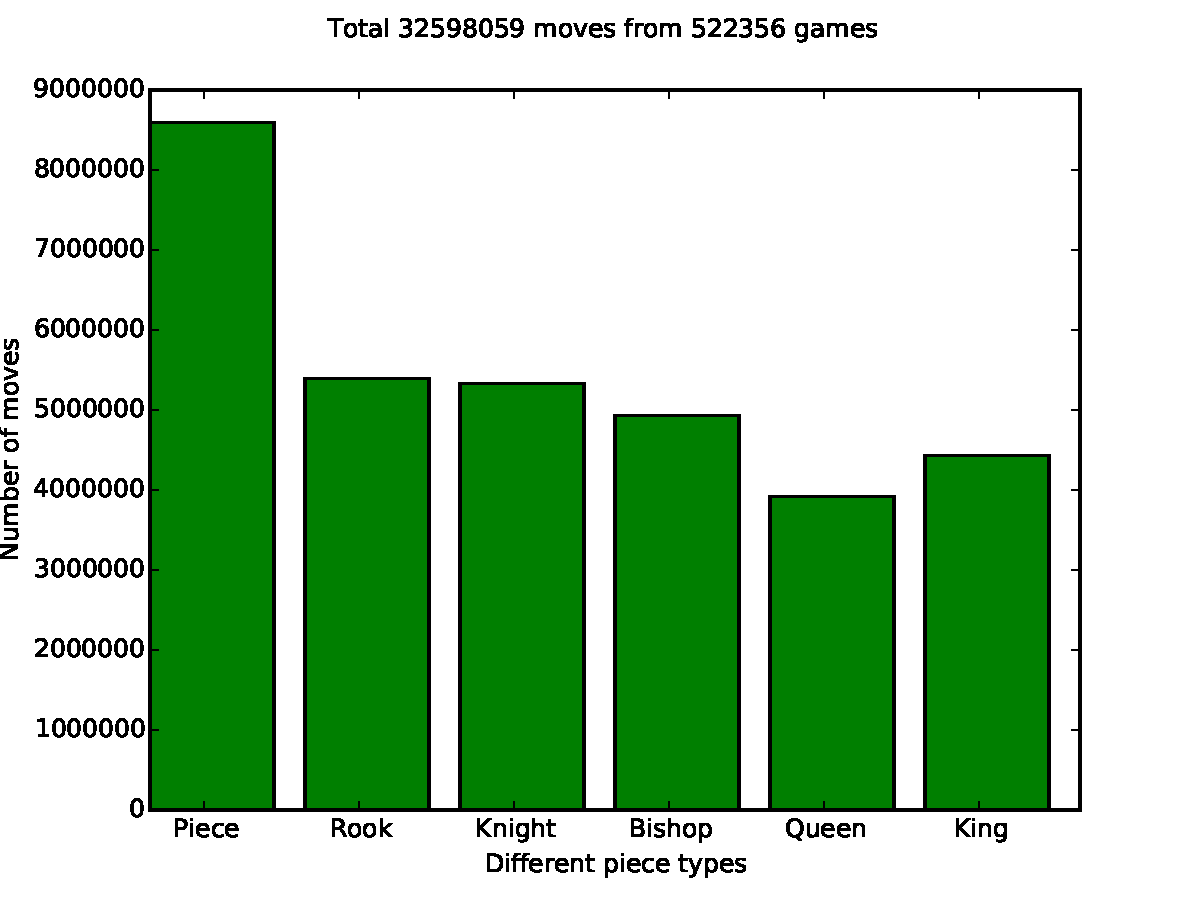
\includegraphics[width=1.0\textwidth,center]{plots/dataset_size_fics.pdf}
%   \caption{Dataset statistics for the FICS(2014) dataset}
%   \label{figure:datasets}
% \end{figure}

\section{Data Representation}
\label{section:datarep}
\subsection{Training data for Piece and Move predictors}
Since we divide our task of evaluating a move into first evaluating the 
position 
of the piece to be played and then evaluating the position to which the piece 
will be played, we represent the data according to the tasks. Effectively, we 
have 7 datasets to train on-- First where the labels are the positions of the 
piece to be played for the input board, and rest of the 6 (for each piece type) 
where the inputs are again the current board positions, but the labels are the 
final positions if any one of that particular type of piece is chosen. We name 
the datasets as-- piece dataset, pawn dataset, rook dataset and so on. 

\subsection{Basic representation}
Following 2 representations were used to represent a chess board:
\begin{enumerate}
\item\textbf{6-channel}: Each board position is represented as 6 channels of 
$8\times 8$ images with values from the set $\{-1,0,1\}$. Each channel 
represents the piece types, namely pawn, rook, knight, bishop, queen, king 
respectively. The friendly player's pieces are represented by a 1 in the 
respective position in the respective channel, while the opponent's pieces are 
represented by a -1 in the respective position in the respective channel. Rest 
of the elements in the $8\times 8$ grid are 0's.\\
Board representation dimensions: $8\times 8 \times 6$\\
\begin{figure}[H]
\centering
\includegraphics[width=0.5\textwidth]{best_moves/output_17_0.png}
\begin{longtable}[width=\textwidth]{ll}
\small
   \begin{tabular}[width=0.33\textwidth]{|llllllll|}
    \hline
    0  & 0  & 0  & 0  & 0  & 0  & 0  & 0  \\
    -1 & -1 & -1 & -1 & -1 & -1 & -1 & -1 \\
    0  & 0  & 0  & 0  & 0  & 0  & 0  & 0  \\
    0  & 0  & 0  & 0  & 0  & 0  & 0  & 0  \\
    0  & 0  & 0  & 0  & 0  & 0  & 0  & 0  \\
    0  & 0  & 0  & 0  & 0  & 0  & 0  & 0  \\
    1  & 1  & 1  & 1  & 1  & 1  & 1  & 1  \\
    0  & 0  & 0  & 0  & 0  & 0  & 0  & 0  \\ \hline
    \end{tabular}
    &
\dots\dots\hspace{0.2cm}
\small
    \begin{tabular}[width=0.33\textwidth]{|llllllll|}
    \hline
    0  & 0  & 0  & 0  & -1  & 0  & 0  & 0  \\
    0  & 0  & 0  & 0  & 0  & 0  & 0  & 0  \\
    0  & 0  & 0  & 0  & 0  & 0  & 0  & 0  \\
    0  & 0  & 0  & 0  & 0  & 0  & 0  & 0  \\
    0  & 0  & 0  & 0  & 0  & 0  & 0  & 0  \\
    0  & 0  & 0  & 0  & 0  & 0  & 0  & 0  \\
    0  & 0  & 0  & 0  & 0  & 0  & 0  & 0  \\
    0  & 0  & 0  & 0  & 1  & 0  & 0  & 0  \\ \hline
    \end{tabular}
  \end{longtable}
\caption{\textbf{6-channel representation} of the initial chess board position}
\small
Leftmost matrix represents the pawn channel. It is followed by the channels 
for Rook, Knight, Bishop and Queen and the rightmost matrix represents the 
king channel.
\end{figure}

\label{section:representation12}
\item\textbf{12-channel}: Each board position is represented as 12 channels of 
$8\times 8$ images with values from the set $\{0,1\}$. Every alternate channel 
belongs to a single player and similar to the 6-channel representation each of 
these channels represents the piece types, namely pawn, rook, knight, bishop, 
queen, king respectively. The friendly player's pieces are represented by a 1 
in 
the respective position in the respective channel, while the opponent's pieces 
are represented by a 1 in the respective position in the respective channel. 
Rest of the elements in the $8\times 8$ grid are 0's.\\
Board Representation dimensions: $8\times 8 \times 12$ (Width, Height, Depth)
\begin{figure}[H]
\centering
\includegraphics[width=0.5\textwidth]{best_moves/output_17_0.png}
\begin{longtable}[width=\textwidth]{ll}
\small
   \begin{tabular}[width=0.33\textwidth]{|llllllll|}
    \hline
    0  & 0  & 0  & 0  & 0  & 0  & 0  & 0  \\
    0  & 0  & 0  & 0  & 0  & 0  & 0  & 0  \\
    0  & 0  & 0  & 0  & 0  & 0  & 0  & 0  \\
    0  & 0  & 0  & 0  & 0  & 0  & 0  & 0  \\
    0  & 0  & 0  & 0  & 0  & 0  & 0  & 0  \\
    0  & 0  & 0  & 0  & 0  & 0  & 0  & 0  \\
    1  & 1  & 1  & 1  & 1  & 1  & 1  & 1  \\
    0  & 0  & 0  & 0  & 0  & 0  & 0  & 0  \\ \hline
    \end{tabular}
    &
\dots\dots\hspace{0.2cm}
\small
    \begin{tabular}[width=0.33\textwidth]{|llllllll|}
    \hline
    0  & 0  & 0  & 0  & 1  & 0  & 0  & 0  \\
    0  & 0  & 0  & 0  & 0  & 0  & 0  & 0  \\
    0  & 0  & 0  & 0  & 0  & 0  & 0  & 0  \\
    0  & 0  & 0  & 0  & 0  & 0  & 0  & 0  \\
    0  & 0  & 0  & 0  & 0  & 0  & 0  & 0  \\
    0  & 0  & 0  & 0  & 0  & 0  & 0  & 0  \\
    0  & 0  & 0  & 0  & 0  & 0  & 0  & 0  \\
    0  & 0  & 0  & 0  & 0  & 0  & 0  & 0  \\ \hline
    \end{tabular}
  \end{longtable}
\caption{\textbf{12-channel representation} of the initial chess board position}
\small
Leftmost matrix represents the White-pawn channel. It is followed by a 
channel for Black-pawns, then two channels each for Rook, Knight, Bishop and 
Queen and the rightmost matrix represents the Black-king channel.
\end{figure}

\end{enumerate}

\subsection{Additional Bias channels}
The dataset provides us with additional information about the players as well 
as 
the game. We try to utilize that additional information by augmenting 
additional 
channels to the board representations. 
\begin{enumerate}
\item \textbf{ELO Layer}: We append an $8\times 8$ channel with the ELO rating 
(normalized) of the player playing the current move. So, if the ELO rating of 
the current player is X, we will augment the $8\times 8$ matrix consisting of 
all values equal to $\frac{X-MINELO}{MAXELO-MINELO}$, where the values of 
MINELO 
and MAXELO are the minimum and maximum ELO ratings of the players in the 
complete dataset. This adds an additional $8\times 8\times 1$ image to the 
input.

\item \textbf{Piece Layer}: Since the task for the move predictor is just to 
predict the final position of a model-specified piece, we provide the move 
predictor learning procedure(s) the actual piece in consideration for the move. 
In particular, we augment an additional channel with all 0s except a 1 in the 
place of the piece being moved.\\
This information makes the learning procedure much more efficient since it no 
longer has to learn, from the data, which piece is moved and is already learnt 
by the piece selector. Adding this channel gives us a more consistent 
probability metric to decide the move (described in~\ref{subsection:topprob}).

This adds an additional $8\times 8\times 1$ image to the input.\\
Although the inclusion of this layer seems intuitive and beneficial, the 
downside to a piece specific channel is that it makes the move prediction 
procedure much slower. This happens because the final position probability 
distribution has to be predicted for all the pieces of the same type 
separately. 
If this layer is not included, we can cache the probability distributions by 
the 
move prediction network for each piece types the first time they are queried. 
Besides this disadvantage, the piece layer increases the prediction accuracy of 
the \textsc{Move} networks. 

\item \textbf{Outcome Layer}: The outcome layer is another dynamic bias layer 
which is appended to the input image layers which indicates the final outcome 
of 
the game corresponding to the player facing the current board position. 
Specifically, we append an image of all ones for a player who finally won the 
game by resignation or check-mate, an image of all zeros for a player who 
finally lost or resigned the game, or an image of all values as $0.5$ for both 
the players if the game was a draw. This adds an additional $8\times 8\times 1$ 
image to the input.\\
The significance of this layer is to give an additional information to the 
model 
which can help evaluating the quality of the move better.\\

\end{enumerate}


\section{Piece and Move Predictor}
\label{section:network-arch}
\begin{figure}[h]
\centering
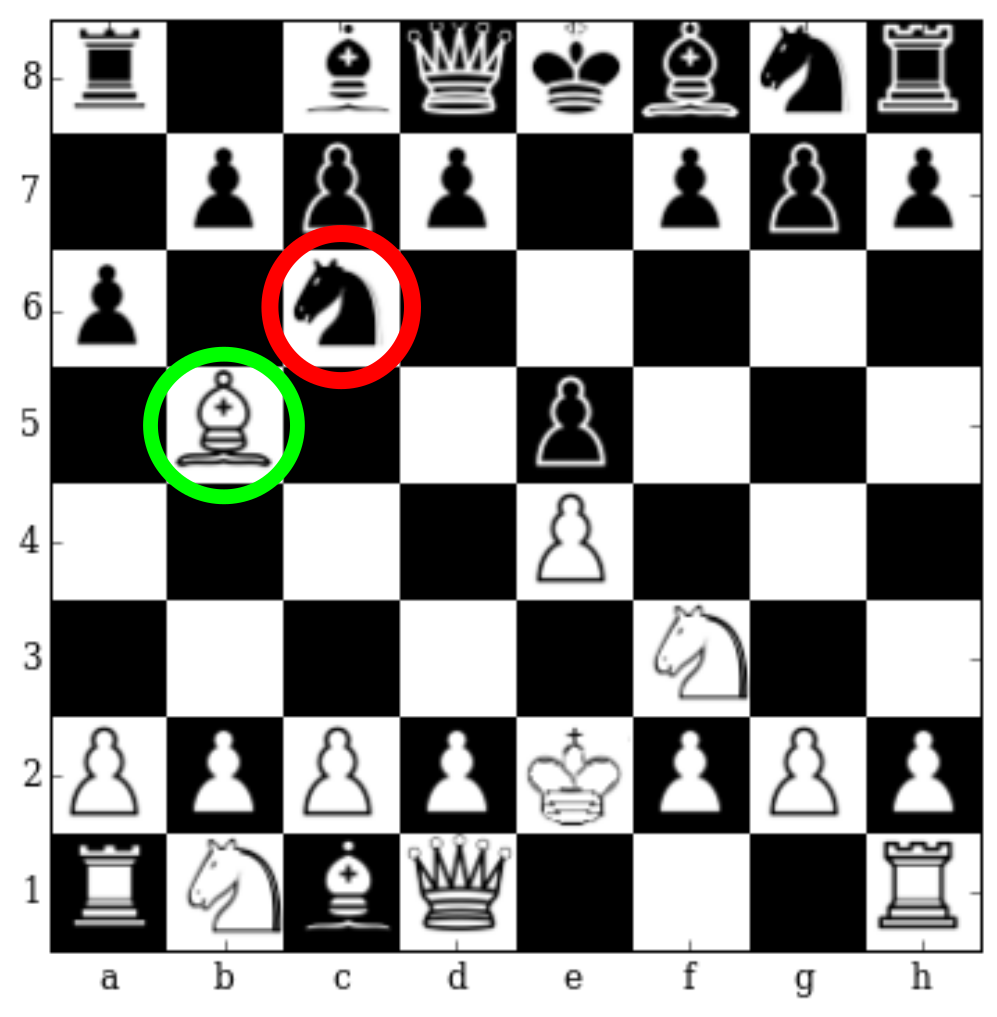
\includegraphics[scale=0.75]{img/from_to.png}
\caption{Model Overview}
\label{figure:model_overview}
\justifying
\small The green circle is the position to be predicted by the \textsc{Piece} 
selector network, while the red circle is the position to be predicted by the 
\textsc{Bishop} move selector network.
\end{figure}
A move in chess is characterized by legal movement of a friendly piece. The 
selected piece is moved onto one of the positions depending on factors like its 
ability to jump over another piece or not, whether the final position already 
has a friendly piece, whether the move doesn't cause a check etc. We divide 
this task into two simple steps--choose a piece, choose its final position. 
Given a board, we predict the next move by simply making the 
predictions in this order. While learning we consider the moves from the 
dataset as gold standard and minimize our loss functions in order to make the 
network learn certain generalizations, rules and even strategies. In 
figure~\ref{figure:model_overview}, the two different colored circles represent 
these two tasks. A formulation of this process would be:
\[P(move | board) = P(from|board)\times P(to|from, board)\]
To learn the probability function, we make use of Convolutional Neural 
Networks. Each of the different types of pieces has its own independently 
trained network, namely-- \textsc{Pawn}, \textsc{Rook}, \textsc{Knight}, 
\textsc{Bishop}, \textsc{Queen} and \textsc{King}, while the piece selector 
network is named \textsc{Piece}.\\

The network used for both piece selector and move selectors are shown below:\\
\begin{figure}[H]
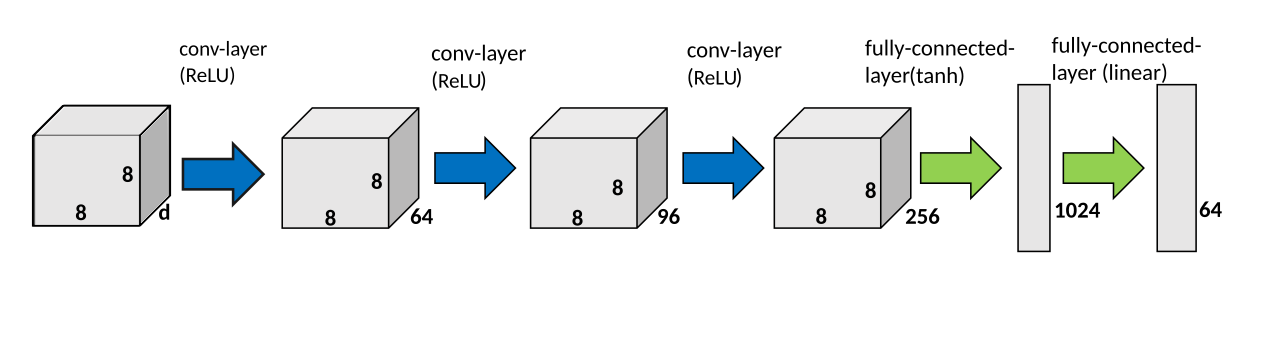
\includegraphics[width=1.0\textwidth,center]{img/net1.png}
\caption{Network Architecture: ChessNet-1}
\small\centering
This network was used for piece and move predictions.
\label{figure:network1}
\end{figure}
The convolutional neural network shown in figure~\ref{figure:network1} consists 
of input layer of size $8\times 8\times 6$ (or $8\times 8\times 12$ depending 
on the choice of representation, described in 
section~\ref{section:representation12}), an output layer of size 64 which 
predicts the position of the piece to be moved. The other specifications of the 
network are:
\begin{itemize}
 \item \textbf{Convolutional Layer}-- 
 \begin{enumerate}
  \item filter size =$3\times 3$ each of depth 6
  \item number of filters=$64$
  \item padding=1
 \end{enumerate}
 \item Non-linearity-- \textbf{ReLU} $max(0,x)$
 \item \textbf{Convolutional Layer}-- 
 \begin{enumerate}
  \item filter size =$3\times 3$ each of depth 64
  \item number of filters=$96$
  \item padding=1
 \end{enumerate}
 \item Non-linearity-- \textbf{ReLU} $max(0,x)$
 \item \textbf{Convolutional Layer}-- 
 \begin{enumerate}
  \item filter size =$3\times 3$ each of depth 96
  \item number of filters=$256$
  \item padding=1
 \end{enumerate}
 \item Non-linearity-- \textbf{ReLU} $max(0,x)$
 \item \textbf{Fully connected layer}-- dimensions=1024
 \item Softmax (Loss) Layer -- \textbf{Softmax}, 
 $p_k=\frac{e^{o_k}}{\sum_i e^{o_i}}$, $o_k$ is the activation at the last 
fully connected layer in the network.
\end{itemize}

While training, the softmax layer is replaced by a softmax loss layer, output 
for the softmax loss layer is defined as follows:
\[L = - \sum_j y_j log p_j\]
where L is the loss, $y_j$ is 0 or 1 depending on the actual 
label.\label{section:lossfunc} The 
derivative of the loss function can be derived as follows:
\begin{align*}
 \frac{\partial L}{\partial o_i} &= -\sum_k y_k\frac{\partial log p_k}{\partial 
o_i} \\
&= -\sum_k y_k \frac{1}{p_k}\frac{\partial p_k}{\partial o_i}\\
&= -y_i(1-p_i) - \sum_{k\neq i} y_k \frac{1}{p_k}(-p_kp_i)\\
&= p_i\bigg(\sum_k y_k\bigg) - y_i\\
&= p_i-y_i
\end{align*}

\section{Learning the evaluation function}
\label{section:eval-func}
In addition to a piece and move predictor, we also learn an evaluation 
function. Since we want to be consistent with not injecting any domain 
knowledge for the game of chess to our models, we formulate the task of 
learning the evaluation function as regression problem with the evaluations of 
the boards inspired by TD-Learning \cite{Barto89learningand, 
sutton1988learning}. Particularly, without using any other knowledge of the 
game, we simply assign discounted reward values to the board as its evaluation. 
Starting with the final leaf nodes (after which no more gameplay is possible or 
one of the player has resigned), we assign board values to be 1 for the winning 
player's board view, -1 for the losing player's board 
view\footnote{Since we are learning from white's perspective, the player's 
board view refers to how the board would have looked to the player if he was 
playing as a white i.e. the board flipped across the horizontal as well 
flipped by color.} and 0 for both if it was a draw. This assignment is the same 
as that 
described as an optimal evaluation function for chess given the fully expanded 
game tree described in~\ref{section:solving}. But for the preceding board 
positions, we assign a discounted reward value as the valuation using a 
discounting factor represented by $\gamma$, where $0\leq \gamma \leq 1$.
\[V(b_{t_{final}}) = \begin{cases}
1 \text{ , if White has won}\\
0 \text{ , if it is a draw}\\
-1 \text{ , if Black has won}
\end{cases}\]
According to the recursive rule the discounted reward for a board at time $t$ 
into the game is:
\[V(t) = \gamma V(t+1) , \forall t<t_{final}\]
Use the following rule moving up into the game:
\[V(b_{t_{final}-i}) = \begin{cases}
		\gamma^{i} \text{ , if white won eventually}\\
                -\gamma^{i} \text{ , if black won eventually}\\
                0 \text{ , if the game was a draw}\\
               \end{cases}\]
\[V(b'_{t_{final}-i}) = \begin{cases}
		-\gamma^{i} \text{ , if white won eventually}\\
                \gamma^{i} \text{ , if black won eventually}\\
                0 \text{ , if the game was a draw}\\
               \end{cases}\]
where $b_{t_{final}-i}$ is the board (as it appears to the white player) $i$ 
steps away from the finish, while $b'_{t_{final}-i}$ is the rotated board with 
flipped colors i steps away from the finish.\\

Since the learning is done offline (in our case using game databases), we 
simulate the whole game before assigning values to each board appearing in the 
board. Now, each board position seen in the data has some evaluation that is 
based on the final outcome of the game. It is intuitive to say that a player who 
is seeing a higher valued board is more likely to win. And higher the value of 
the current board, the closer I am to winning the game and vice versa.\\

We model the task of learning such an evaluation function as regression problem 
on the network shown in figure~\ref{figure:network2}.
\begin{figure}[h]
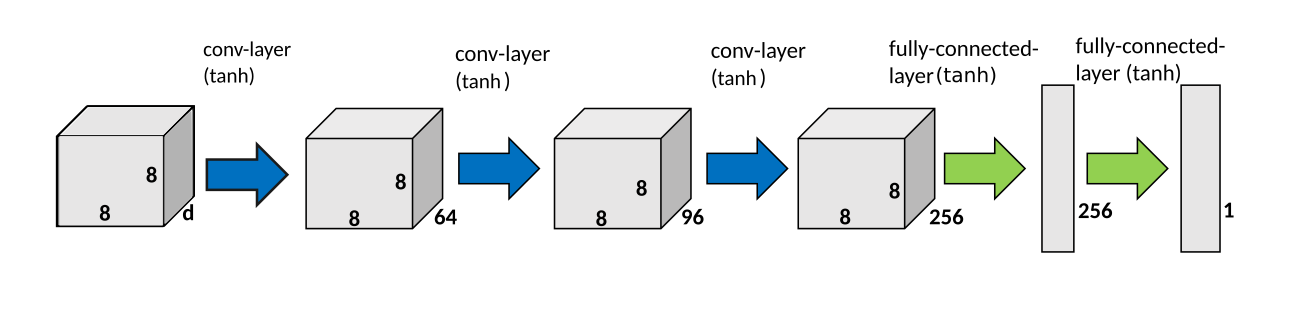
\includegraphics[width=1.0\textwidth,center]{img/net3.png}

\caption{Network Architecture: ChessNet-2}
\small\centering
This network was used for regression to learn the evaluation function. The 
difference from the network in~\ref{figure:network1}, other than the dimensions 
of output, is the type of non-linearity used. In this network we use $tanh$, 
rather than ReLU since we need values to range from -1 to 1. We also tried 
other non-linear activation functions like leaky ReLU or a sigmoid function 
with no significant difference in results.
\label{figure:network2}
\end{figure}

The input layer size is $6\times 8\times 8$, while the output layer size is 1 
i.e. the evaluation function's value for the input board. The loss function 
optimized to train the network is the \textit{mean squared error} which is the 
basic linear regression loss function.
\[L = \frac{1}{2}(f(x)-y)^2\] where x is the value at the last fully 
connected layer in the network and f is the activation function (tanh in our 
case).
Simply the gradient looks like:
\[\frac{\partial L}{\partial x} = (f(x)-y)\frac{\partial f(x)}{\partial x}\]

The backward pass for rest of the layers works in the same way as the previous 
network.

\section{Playing}
\label{section:playing}
In this section we will look at the algorithms we use during the gameplay to 
decide which move to play depending on the outputs of our models. The first two 
algorithms do not make use of search and just make predictions based on the 
current table, while the rest mix the predictions or evaluations made by our 
model with a search based mechanism to predict the next move.

\section{Choosing a move}
The output by each of the networks for a given input board (with or without the 
augmented channels) is a probability distribution over the whole board. The 
probability distribution output by the trained \textsc{Piece} network, call it 
$P_{piece}$, is a 64-dimensional vector where each value denotes the probability 
of moving the piece at the corresponding position on the board. Similarly, the 
probability distribution output by the $i^{th}$ \textsc{Move} network, call it 
$P_{move,i}$, is a 64-dimensional vector where each value denotes the 
probability of moving a piece of type $i$ to that particular position. We use 
two or more of these probabilities to choose the complete move (initial and the 
final position) using one of the methods described below.
\subsection{Top-move method}
Simply choose the piece at position with the maximum probability in the 
\textsc{Piece} network's output. Determine its piece type and input the same 
board to the type's \textsc{Move} network. Choose the final position with the 
maximum probability.
\begin{algorithm}[H]
\begin{algorithmic}[1]
 	\State initial\_pos = argmax($P_{piece}(board)$)\;
   	\State piece\_type = getType(initial\_pos)\;
   	\State final\_pos = \funccall{argmax}($P_{move,piece\_type}(board)$)\;
   	\Return chess\_coords(initial\_pos)+chess\_coords(	final\_pos)\;
\end{algorithmic}
\caption{Top-move method}
\label{alg:topmove}
\end{algorithm}

\subsection{Top-prob method}
\label{subsection:topprob}
Rather than just determining the distribution of the moves originating from the 
most probable piece, we can also generate the full cumulative probability 
distribution for every possible from-to pair. This method is based on the 
principle that: 
\[P(move | board ) = P(piece | board )\times 
P(final\_position|piece, board)\]

\begin{algorithm}[H]
 \begin{algorithmic}[1]
 	\State piece\_dist = $P_{piece}(board)$
   	\State cumulative\_dist = \funccall{zeros}(64,64)
   	\For {$0\leq i<64$}
   		\If {$board[i/8,i\% 8]\neq 0$}
   			\State piece\_type=\funccall{getType}(i)
   			\State move\_distr = $P_{move,piece\_type}(board)$ * 
piece\_distr[i]
   			\State cumulative\_distr[i] = move\_distr
   		\EndIf
   	\EndFor
   	\State initial\_pos, final\_pos = \funccall{argmax}(cumulative\_distr)
   	\Return \funccall{chess\_coords}(initial\_pos)+\funccall{chess\_coords}	
(	final\_pos)
 \end{algorithmic}
 \caption{Top-prob method}
 \label{alg:topprob}
\end{algorithm}

\subsection{TopProb-Negamax Interleaved}
\label{subsection:interleaved}
In this method we interleave our method of evaluating moves with negamax, which 
is a kind of minmax search algorithm. We will 
describe both Negamax and our pruning method interleaved with Negamax.
The basic idea is that we will reduce the search space for the Negamax 
algorithm and also provide it with an evaluation metric for the moves or the 
boards.\\
%XXX
The Negamax algorithm is derived from Minimax algorithm. However it differs in 
the way that it utilizes the same subroutine for the Min player and the Max 
player at each step, passing on the negated score following the rule:
\[max(a,b) = -min(-a,-b)\]
\begin{algorithm}[h]
 \begin{algorithmic}[1]
 	\Procedure{Negamax}(depth)
 	\If {depth==0} 
	  \Return \funccall{evaluate}()
 	\EndIf
 	\State max = $-\infty$
 	\State \funccall {generateMoves}($\dots$)
 	\While {m = \funccall{getNextMove}()}
	  \State \funccall{makeMove}(m)
	  \State score = -\funccall{Negamax}(depth -1)
	  \State \funccall{unmakeMove}(m)
	  \If {score $>$ max}
	    \State max = score
	  \EndIf
	\EndWhile
	\Return max
    \EndProcedure
 \end{algorithmic}
 \caption{The basic Negamax algorithm for Chess}
 \label{alg:negamax}
\end{algorithm}
 The functions $makeMove$ and $unmakeMove$, as the names suggest, make the move 
on the board before calling Negamax again for the child nodes, and then un-make 
the move to search the subtrees of the siblings.

However, the function calls of our interest is the $generateMoves$ and 
$evaluate$. $generateMoves$ function uses chess logic to generate 
legal moves, which are then explored using recursion, while $evaluate$ uses the 
player's evaluation function to return the value for a leaf node.\\

For our case, we can modify the $generateMoves$ procedure to actually just 
generate a reduced number of moves available at every board position, hence 
pruning the search tree. The reduced number of moves are generated in a way 
similar to algorithm~\ref{alg:topprob}, where we generate a 
cumulative probability distribution of size $64\times 64$. The difference being 
that rather than making a move, we just explore the subtree of the generated 
move. In the same way as before, we can make use of transposition tables to 
store the values of boards already evaluation while expansion of the tree.\\

Our idea of making a narrower and deeper search of the game tree instead of a 
full width and shallow search is motivated by \citealp*{de1996perception} as 
discussed in chapter~\ref{chap:background}.\\

For $evaluate$ function call, we simply ask our network to evaluate one or a 
batch of boards. The function is better described earlier in 
the section~\ref{section:eval-func}.

\section{Training: Implementation details and Hyper parameters}
\label{section:hyperparams}
We performed all our training and testing for the piece and move prediction 
models on a deep learning library named Caffe \cite{jia2014caffe} using its 
Python API. However, we couldn't use Caffe for the 
regression training and related experiments because of convergence issues. The 
implementation for the regression training to learn the 
evaluation function was done using a Theano-based deep learning library named 
Keras \cite{keras}. The complete source code of our implementation is available 
on \url{https://github.com/ashudeep/convchess}. \\

All the experiments were run on a machine with NVIDIA GeForce GTX 760 GPU with 
Cuda v6.5.\\

Move prediction models: We experimented with different hyperparameters for the 
learning procedure and 
obtained our best models at: base learning rate  of $\alpha=0.1$ and a batch 
size of 1000. We used AdaGrad to compute the updates. The learning rate was 
kept 
constant for the first $50,000$ iterations before reducing it to 0.01. The move 
prediction networks in Caffe were trained uptil $300,000$ iterations which took 
about 2-3 days.\\

Evaluation Function learning: We used a learning rate of 0.001 and RMSprop with 
a learning rate decay of 0.9 to minimize the mean squared error. We use a batch 
size of 1024. We varied the values of $\gamma$ (described in section 
\ref{section:eval-func}) between 0.7 and 0.99 to train separate models. The 
results and analysis for each of them are described in this chapter.\\

	\chapter{Results and Analysis}
\label{chap:results}
The two primary components of a chess playing system are: \textbf{evaluation 
function} and \textbf{search}. In chapter \ref{chap:background} we already 
looked at these two aspects of the conventional chess playing systems and how 
the exponential increase in computational power has led to better search-based 
methods, due to which we have computer chess systems that can beat the best 
humans. Our aim here is not to build such a system, but to provide a proof of 
concept that Convolutional Neural Networks, one of the most powerful pattern 
recognition architecture, can observe patterns from chess games and eventually 
learn to play chess. As described in chapter \ref{chap:implementation}, we use 
CNN to learn an evaluation function and a move predictor directly from 
chess games with minimum injection of chess knowledge to the predicted 
probabilities. In this chapter, we empirically evaluate these CNN based models 
on their ability to play chess. 
% The primary contribution of our work is to provide a better evaluation metric 
% for evaluating chess boards and hence moves. Another contribution is to prune 
% the moves before search using a pre-trained model, so that the enormous search 
% space for a conventional chess playing algorithms are reduced considerably. We 
% show the results that demonstrate these contributions.

\section{Training}
Figure \ref{figure:losses} and \ref{figure:losses-accuracies} show the training 
loss and test loss during training of the \textsc{Piece} prediction models. The 
plots for the move prediction models of different pieces are similar and hence 
omitted for brevity. The loss function plotted below is defined by:
\[L = - \sum_j y_j log p_j\]
where L is the loss, $y_j$ is 0 or 1 depending on the actual label. This is the 
function we minimize while training and has been discussed in 
section~\ref{section:lossfunc} 
\begin{figure}
\vspace*{-0.5in}
  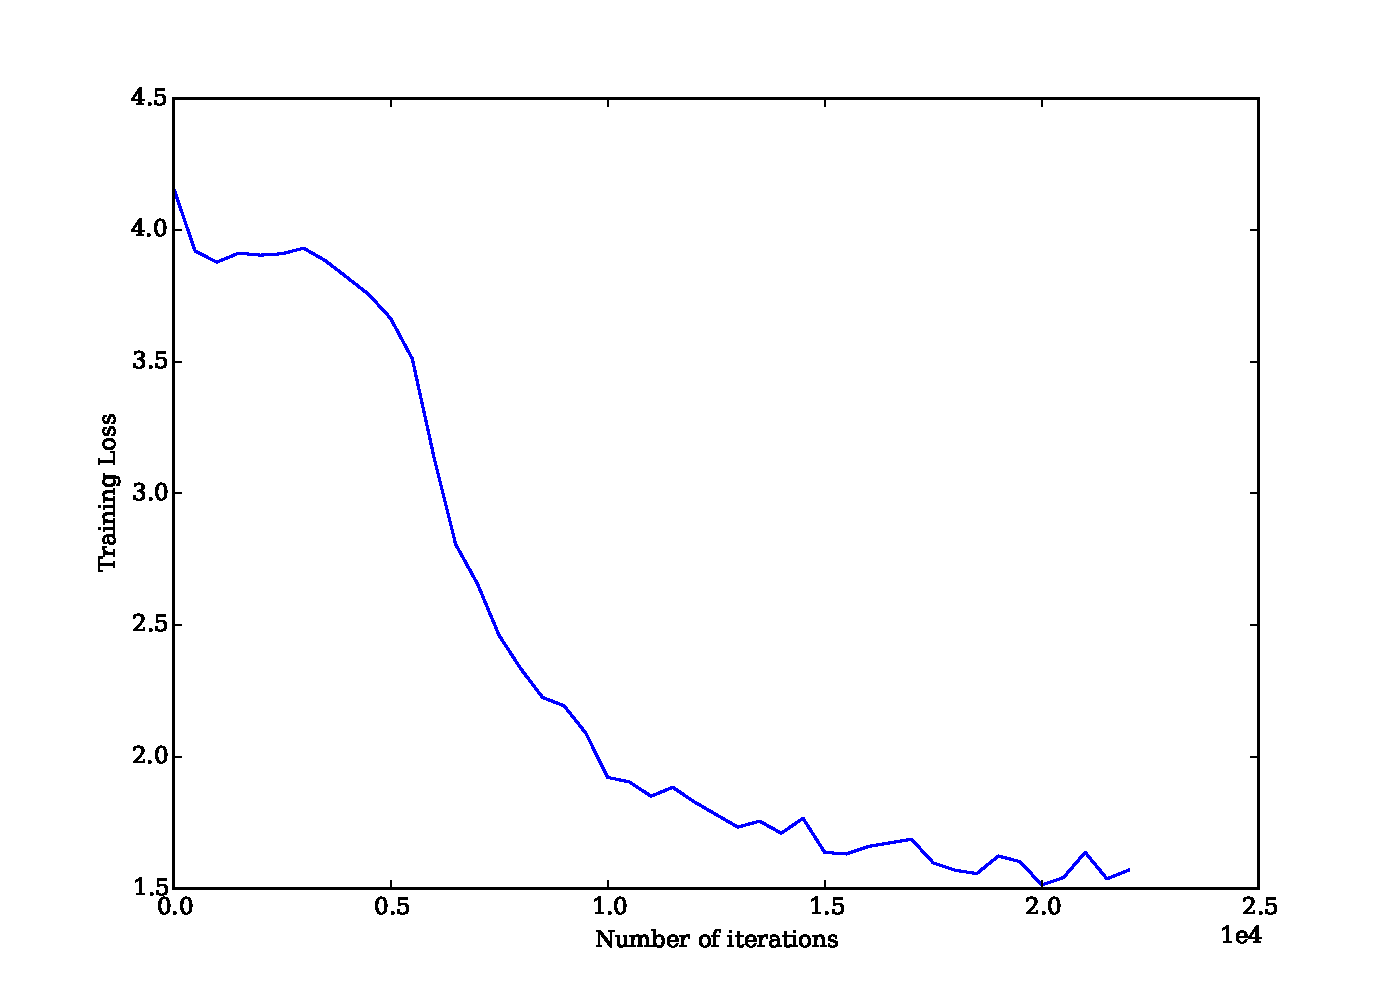
\includegraphics[width=1.0\textwidth,center]{plots/training_curve_new.pdf}
  \caption{Variation of the softmax-loss while training of 
\textsc{PIECE} model}
  \label{figure:losses}
\end{figure}
\begin{figure}
  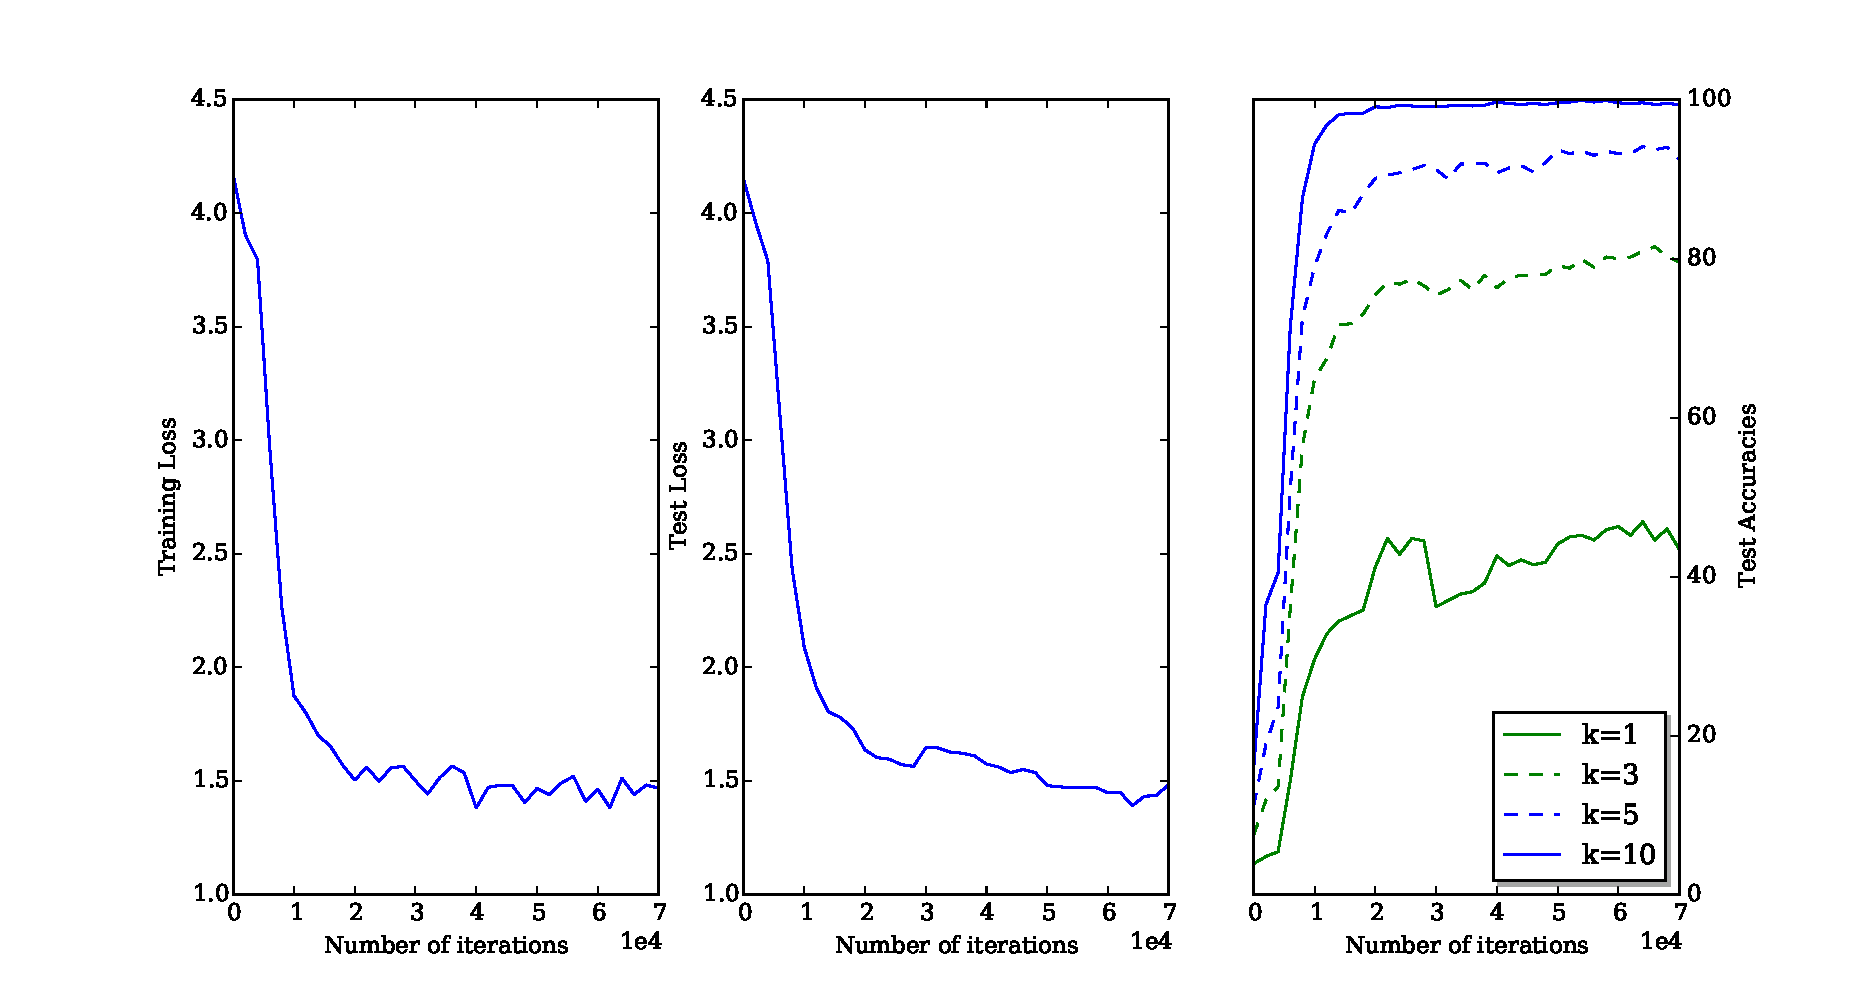
\includegraphics[width=1.55\textwidth,center]{plots/learning_curve_new.pdf}
  \caption[Variation of the accuracies on test set while training]{
  (a) Softmax-loss on training dataset (b) Softmax-loss on 
testing dataset; (c) Accuracies at k=1,3,5,10 on testing dataset.}
  \label{figure:losses-accuracies}
\end{figure}
%\section{Network Filters}

\section{Performance of \textsc{Piece} and \textsc{Move} networks}
As discussed in Chapter \ref{chap:dataset}, we divided the dataset into training 
and testing sets. We train the network, using the optimum hyper-parameters 
described in section \ref{section:hyperparams}.\\
%parameters here
The training and testing accuracies and softmax losses have been reported in the 
table below. We also report the top-k prediction accuracies for $k=3,5,10$ 
also. 
%We also compare 
% the top piece's and top move's average probability in each of the networks along 
% with the average rank of the actual move.
\begin{table}[H]
\centering
\begin{tabular}{@{}lllll@{}}
\toprule
\multirow{2}{*}{Model Name} & \multicolumn{4}{c}{Accuracy at k}                  
                                                    \\ \cmidrule(l){2-5} 
                            & \multicolumn{1}{c}{k=1} & \multicolumn{1}{c}{k=3} 
& \multicolumn{1}{c}{k=5} & \multicolumn{1}{c}{k=10} \\ \midrule
Piece                       & 56.0                    & 87.9                    
& 95.8                    & 99.5                     \\
Pawn                        & 94.8                    & 100.0                   
& 100.0                   & 100.0                    \\
Rook                        & 58.0                    & 85.2                    
& 93.5                    & 99.6                     \\
Knight                      & 77.3                    & 96.6                    
& 99.3                    & 100.0                    \\
Queen                       & 54.2                    & 81.3                    
& 90.4                    & 98.2                     \\
King                        & 71.7                    & 95.6                    
& 99.6                    & 100.0                    \\ \bottomrule
\end{tabular}
\caption{Test set performance without masking}
\label{table:performance}
\end{table}


\section{Performance after masking}
\label{sec:masking}
We hypothesize that the model will eventually learn the rules of chess through 
observation only. In this section, we will try to demonstrate how good our model 
performs in learning the rules of the game of chess.\\

Since the model has no prior information of the rules of the chess game, we can 
expect the model to make some mistakes by predicting an illegal move. For a 
legal gameplay, we use the method of \textbf{masking} the probabilities. Masking 
is done at two levels due to the inherent design of our method. First, we zero 
the probabilities of the piece positions which do not contain a friendly piece. 
Secondly, we zero out the probabilities of the final positions where the chosen 
piece type cannot reach using a single valid move.\\

After masking the probabilities for each of the board positions, we compare 
our results with the unmasked predictions to demonstrate how well our model 
has learnt the rules of chess.

\subsection{Rule learning and move legality}
We discussed how injection of chess knowledge into predicted probabilities can 
ensure that we obtain legal moves while playing. However, we also 
hypothesized that the model eventually learns the rules of the game. We will 
demonstrate this further by comparing the probability distributions obtained 
before and after masking. We use two measures to calculate the similarity 
between two distributions-- Chebyshev similarity and squared euclidean 
distance. The 
distance metrics are computed using the following expression:
\[D_{sqeuc}(p,q) = ||p-q||^2\]
\[D_{chebyshev}(p,q) = \max_{i}|p_i-q_i|\]
Both the measures are symmetric. Chebyshev distance is intuitively the maximum 
zeroed out probability value from the unmasked distribution, while the 
euclidean distance is a common measure to estimate the distance between the two 
probability vectors in the n-dimensional space (n=64 in our case). We didn't 
use KL-divergence, which is the most common measure to compute dissimilarity 
between probability distributions, since we have zero probabilities.\\

We run our experiments on a relatively small dataset of 314,740 boards and 
report the average squared euclidean distance, average Chebyshev distance 
between masked 
and unmasked probability distributions and the average number of illegal 
predictions in the table below.
\begin{table}[H]
\centering
\begin{tabular}{@{}llllll@{}}
\toprule
{\bf } & $||p-q||^2$ & $\max_i |p_i-q_i|$& Illegal move& 
\multicolumn{2}{l}{Avg Rank of actual move} \\ \cmidrule(l){5-6} 
{\bf Model}           &        &             &\%age                        & 
unmasked          & masked          \\ \midrule
{\sc Piece}  &     $3.09\times 10^{-8}$ & $4.28\times 10^{-5}$                 
    & 0.0 &2.06342060113 &2.06341424668                   
\\
{\sc Pawn}   &     $1.72\times 10^{-4}$               & $5.82\times 10^{-4}$    
                  & 0.0045 &       1.08001395504 &1.07996844947             
\\
{\sc Rook}   &             $3.74\times 10^{-3}$& $1.37\times 10^{-2}$           
 &   0.72       &2.31513493742 &2.28972185557           
\\
{\sc Knight} &       $1.74\times 10^{-5}$             &     $4.8\times 
10^{-4}$                  &       0.0 & 1.44417866616 &1.44410761652            
  
\\
{\sc Bishop}  &    $3.94\times 10^{-3}$                &  $1.15\times 10^{-2}$  
 
& 0.47                 &  1.83962121376 & 1.82638963959         
\\
{\sc Queen}  &     $5.49\times 10^{-3}$               & $1.89\times 10^{-2}$ &  
   1.23                &                   2.52614094756 &2.47512457486  
\\
{\sc King}   &    $3.35\times 10^{-3}$                &   $3.82\times 10^{-3}$ 
&       0.33            &      1.59097552371 & 1.5873805164        
\\ \bottomrule
\end{tabular}
\caption{Rule Learning}
\small\justifying
Distances between predicted probabilities and average 
percentage of illegal predictions
\label{table:rule-learning}
\end{table}
\begin{table}[H]
\centering
\begin{tabular}{@{}lll@{}}
\toprule
\multirow{2}{*}{Model} & \multicolumn{2}{l}{Percentage Accuracy} \\ 
\cmidrule(l){2-3} 
                       & before masking      & after masking     \\ \midrule
Piece                  & 56.11               & 56.11             \\
Pawn                   & 53.60               & 53.60             \\
Rook                   & 50.98               & 51.26             \\
Knight                 & 72.77               & 72.77             \\
Bishop                 & 59.89               & 60.13             \\
Queen                  & 47.99               & 48.42             \\
King                   & 64.49               & 64.76             \\ 
\bottomrule
\end{tabular}
\caption{Rule Learning: Accuracies before and after masking.}
\small\justifying
In the table above, the accuracies of each of the models is compared before 
and after masking for the set of $314,740$ board positions.
\label{table:rule-learning-2}
\end{table}

In the tables~\ref{table:rule-learning} and ~\ref{table:rule-learning-2}, we 
noticed that the models predict a legal move almost every single time when we 
are not masking the probability distributions for legal moves. This is a very 
strong result since one of the hypothesis of our work was whether the dynamics 
of chess are caused by the interactions of the pieces and the patterns they 
exist in. The convolutional neural network based models, which have no prior 
knowledge of the game of chess, can predict a legal move every single time after 
a few tens of  million games where only one in every $10^{36}$ board 
configurations has the exposed to the network. Conclusively, we can say that the 
networks which are trained on move optimality also optimize move legality, 
probably because of their extreme representation power.\\

\subsection{Evaluating performance of full move prediction}
Till now we evaluated our networks individually for piece and move prediction 
tasks. Now, we need evaluate our models in an ensembled fashion to predict the 
entire move, i.e. from and to position on the board. For this task, we evaluate 
predictions for each move as the games in our test dataset proceed. The 
plot in figure~\ref{figure:gameplay1} shows the variation of accuracy of the 
correct move (piece and destination position combined) lying in top-k 
predictions (k=1,5,10,20,30) with the index of the move into the game. The plot 
in figure~\ref{figure:gameplay2} shows the variation of mean accuracy for the 
correct move to lie in the top-k predictions (k is on the x-axis). The moves 
were predicted using the algorithm described in~\ref{alg:topprob}.
\vspace*{-1.5in}
\begin{figure}[H]
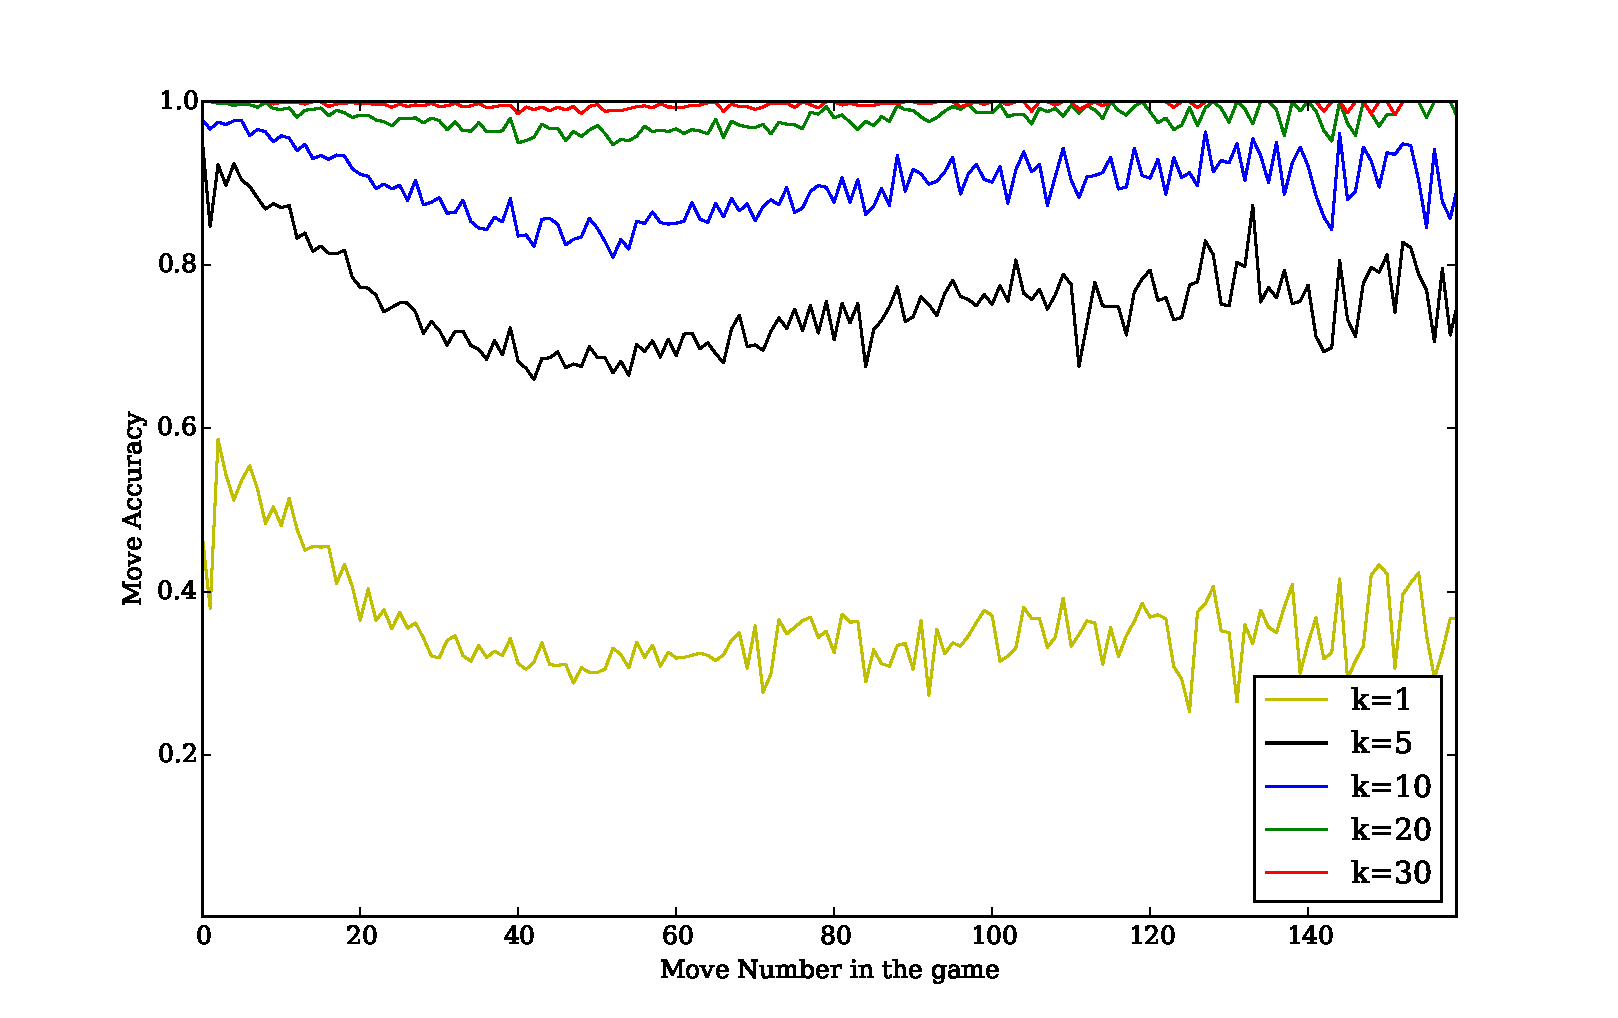
\includegraphics[width=1.3\textwidth,center]{plots/accuracy_new.pdf}
\caption[Variation of accuracies with move number]{Average accuracies at 
different move numbers in test dataset games for top k 
predictions (k=1,5,10,30).}
\label{figure:gameplay1}
\end{figure}
% \begin{figure}
% 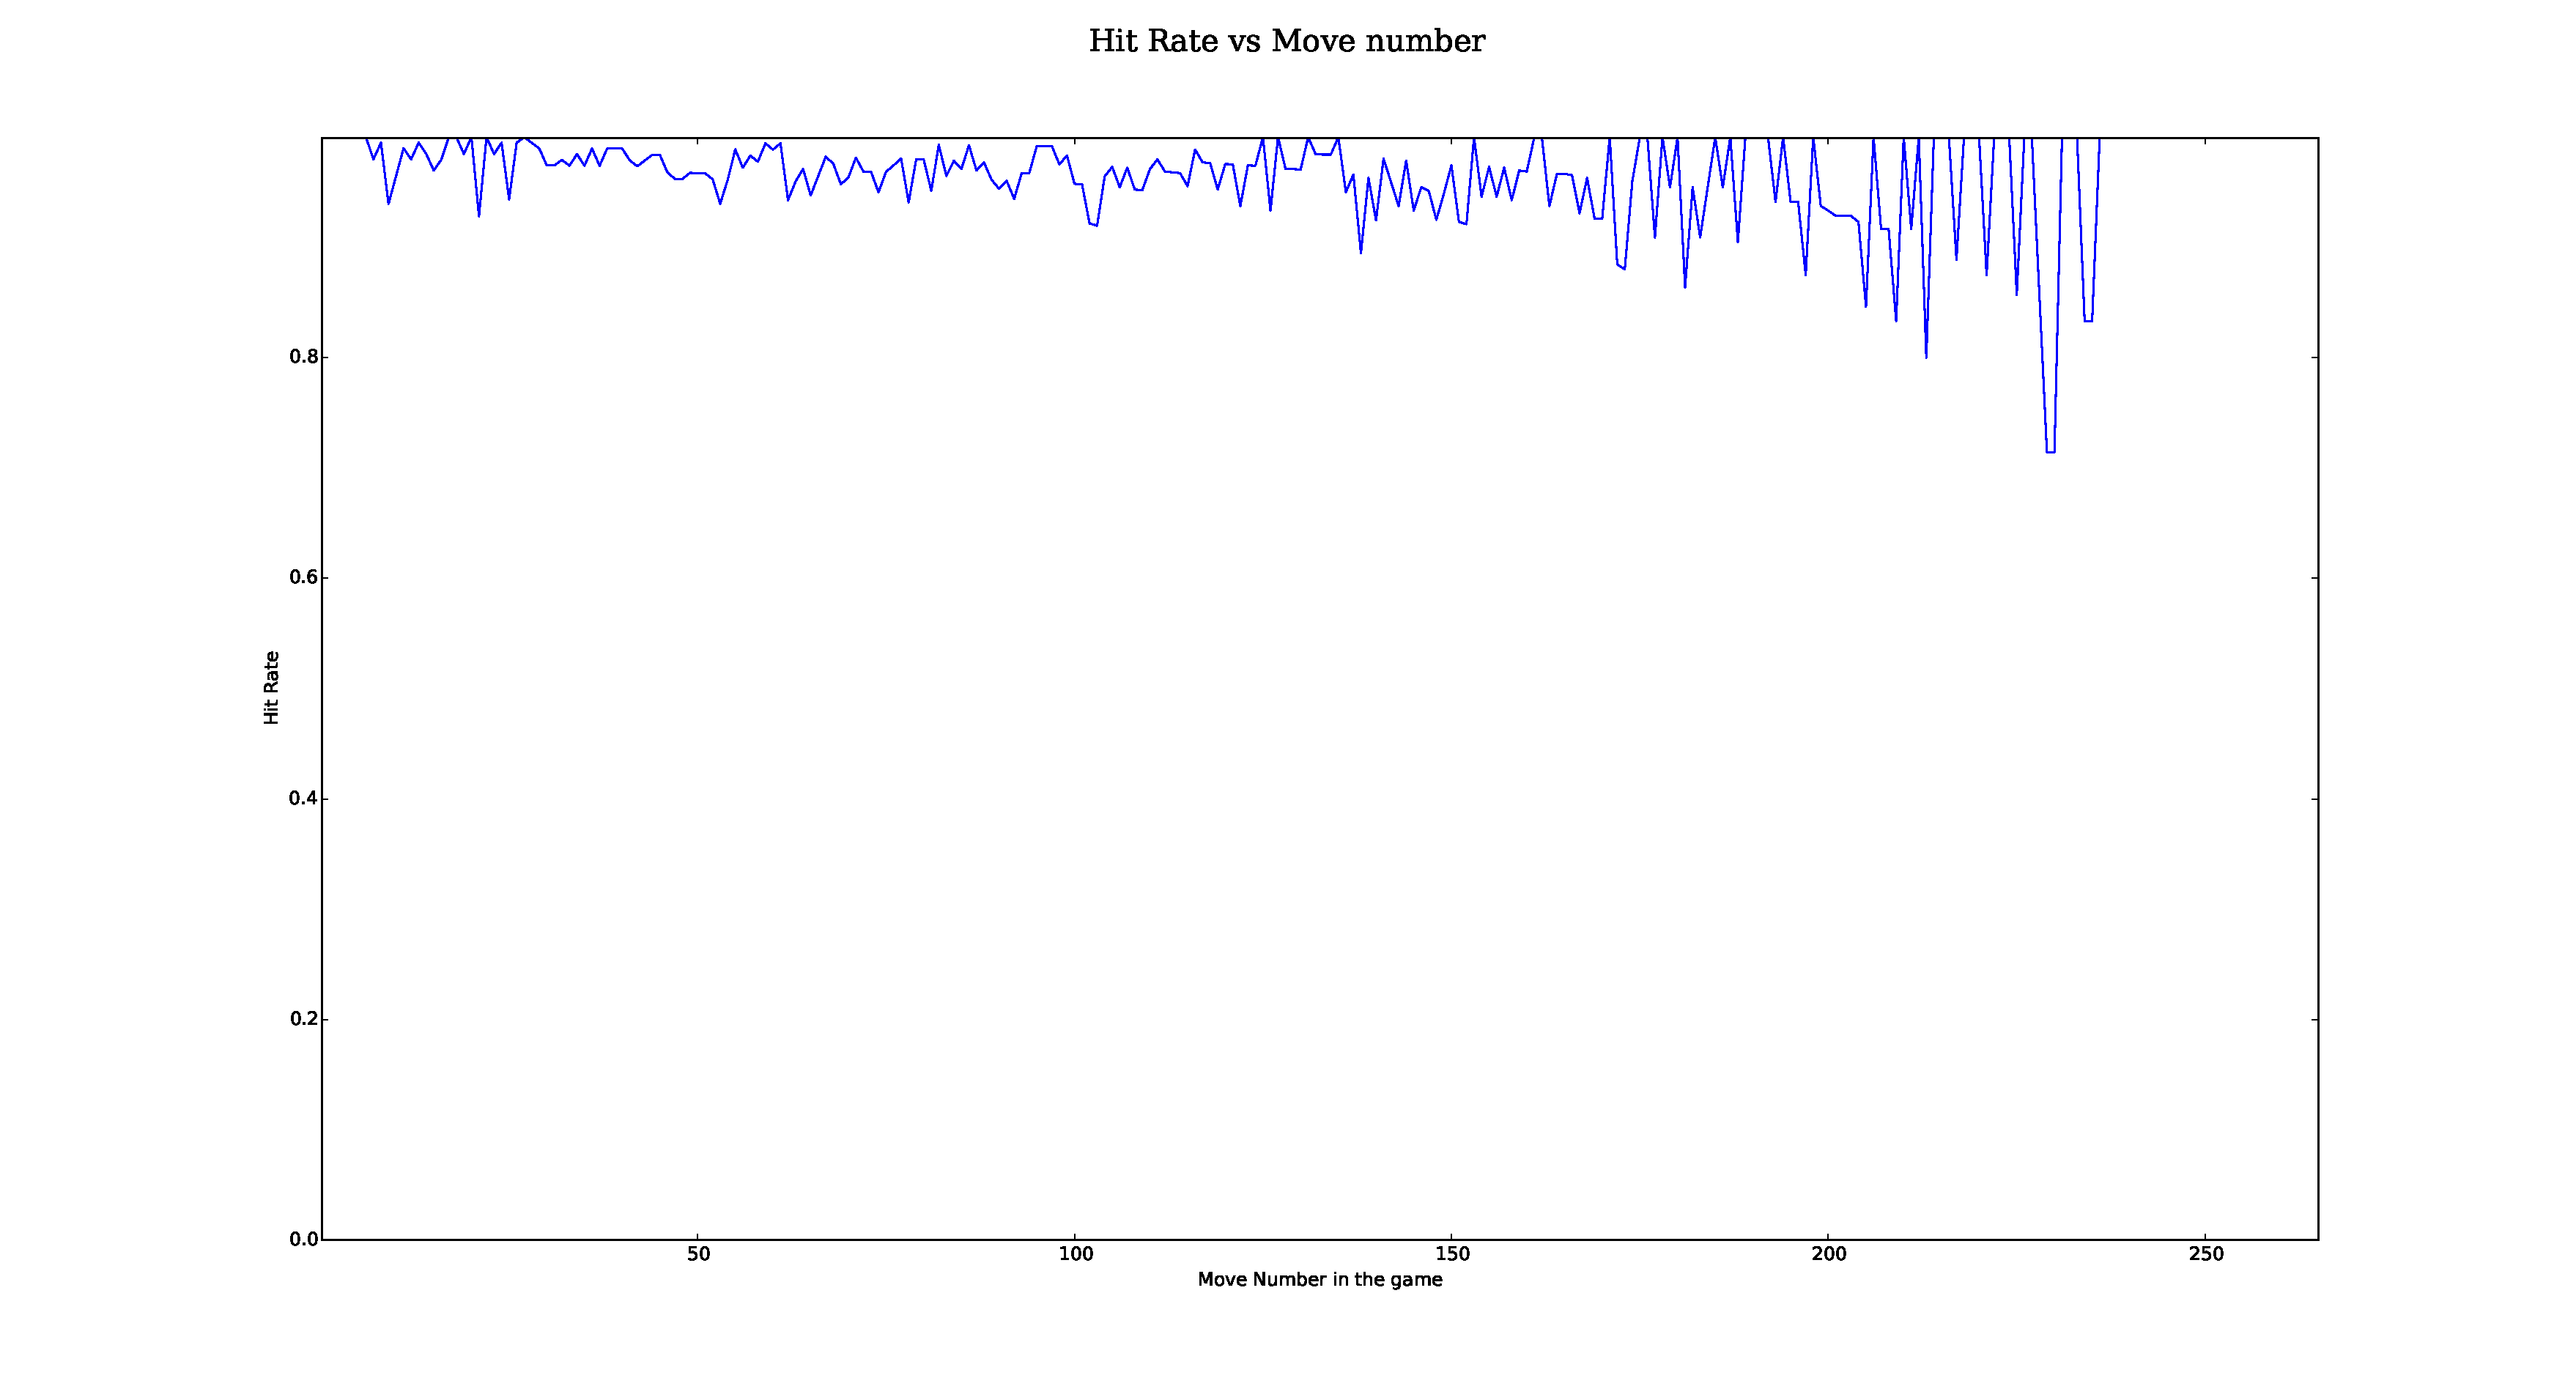
\includegraphics[width=1.5\textwidth,center]{plots/hitrate.pdf}
% \caption{Legal Move rate vs Move Number}
% \label{figure:gameplay2}
% \end{figure}
%\vspace*{-1.0in}
\begin{figure}[H]
  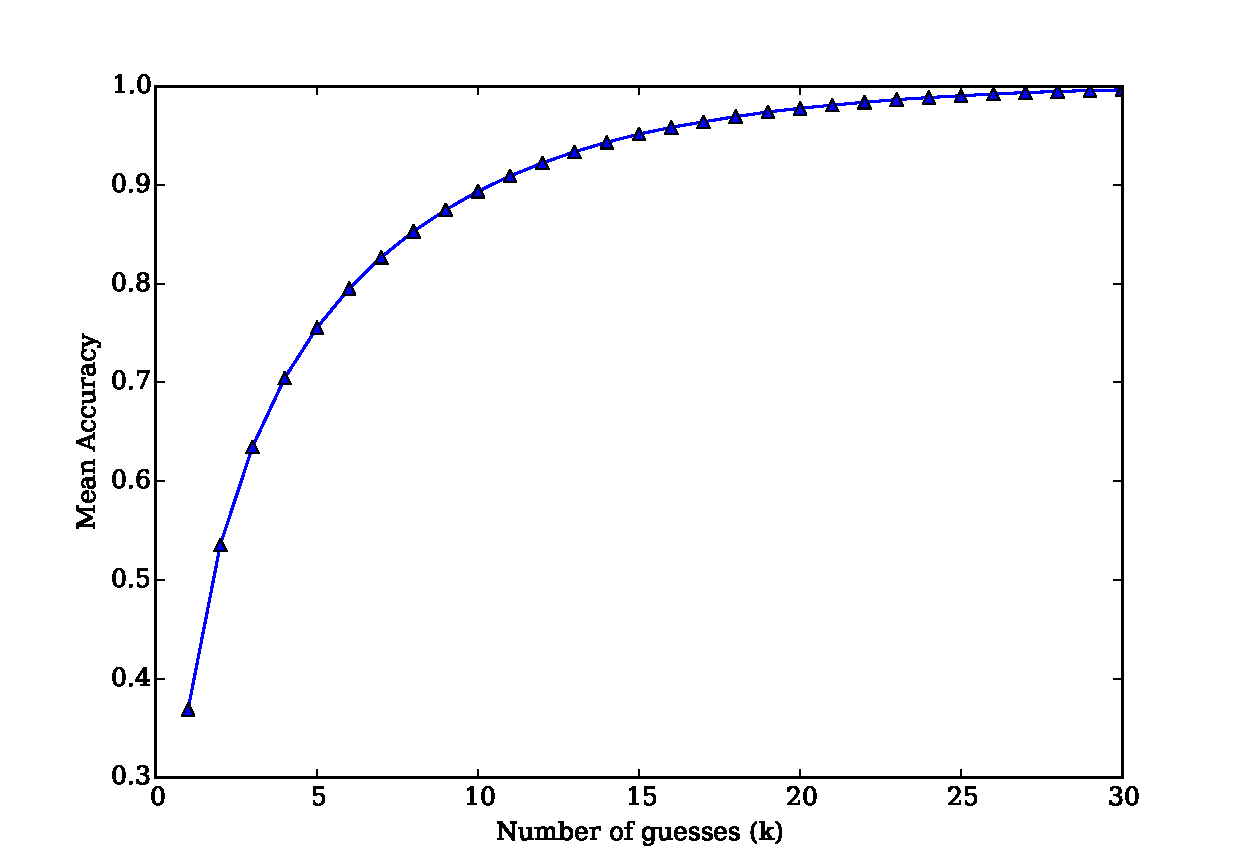
\includegraphics[width=1.0\textwidth,center]{plots/accuracy2_new.pdf}
  \caption[Variation of Top-k accuracy with k]{
  Plot of the variation of mean accuracy of the actual move lying in the 
top-k predictions with k (the number of guesses).}
  \label{figure:gameplay2}
\end{figure}
As we increase $k$ from 1 to 30, the error diminishes to less than 1\%. This 
means 1 in every hundred moves doesn't lie in top 30 of our predictions. We 
suspect that the error is caused, mostly in the middle game when a large number 
of moves are possible and the actual move played is a tactical one with a long 
term strategy in mind.
%XXX how significant is this error

\section{Sample moves taken by the network}
\label{section:samplemoves}

Here are a sample of moves predicted by the network for the board positions. We 
present two cases where the model was asked to predict the probability 
distributions for the ``from'' positions and ``to'' positions for some of the 
pieces on the board. In all the figures below, the chess board used as an input 
to the piece and move predictors. The 64-sized probability distributions are 
visualized as $8\times 8$ matrices with a color bar on the right of each. The 
probability values shown in the move selector distribution are the joint 
probabilities of piece and move selection for that specific move. 
\subsection{Initial board position}
% \vspace*{-0.5in}
We evaluate our piece and network predictors on the initial board position of a 
chess game. Figure~\ref{figure:initialboarda} shows the board position. 
Figure~\ref{figure:initialboardb} shows the distribution of the 
probabilities for the piece to be moved. Note that only the pieces in the second 
rank and the knights in the last rank can move which is apparent in the 
predictions. Table~\ref{table:initialboard} shows the comparison of the 
predicted probabilities and the percentage times the opening move was played in 
the dataset. Bobby Fischer said: ``Best by test: 1.e4'', and we shall 
see this.

\begin{figure}[H]
  \centering
    \begin{subfigure}[t]{0.5\textwidth}
        \centering
        
	\includegraphics[scale=0.7]{img/best_moves/output_17_0.png}
        \caption{Board position(B)}
        \label{figure:initialboarda}
    \end{subfigure}%
  ~
    \begin{subfigure}[t]{0.5\textwidth}
        \centering
        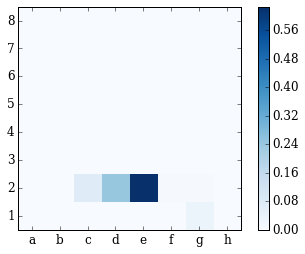
\includegraphics[width=\textwidth]{img/best_moves/output_12_0.png}
        \caption{$P_{\textsc{piece}}(B)$}
        \label{figure:initialboardb}
%         Predicted probability distribution\\
%         for the ``from'' position\\
%         predicted by \textsc{PIECE} network}
    \end{subfigure}
\caption[Predictions for initial board position]{
    (a) The initial board position for a chess game, 
    (b) The predicted probability distribution for the ``from'' piece by the 
\textsc{PIECE} network}
\label{figure:initialboard}
\end{figure}
% Please add the following required packages to your document preamble:
% \usepackage{booktabs}
\begin{table}[]
\centering
\begin{tabular}{@{}llll@{}}
\toprule
Move & Predicted Probability & Number of times played & \%age times played \\ 
\midrule
All  & 1.0000000             & 4970725                & 100.00\%           \\ 
\midrule
e2e4 & 0.6088475             & 2221439                & 44.7\%             \\
d2d4 & 0.2467637             & 1618291                & 32.6\%             \\
c2c4 & 0.0725896             & 286295                 & 5.8\%              \\
g1f3 & 0.0334573             & 334741                 & 6.7\%              \\
e2e3 & 0.0171652             & 62744                  & 1.3\%              \\
f2f4 & 0.0059381             & 67248                  & 1.4\%              \\
g2g3 & 0.0052637             & 93072                  & 1.9\%              \\
b1c3 & 0.0021147             & 98306                  & 2\%                \\
b2b3 & 0.0013837             & 64692                  & 1.3\%              \\
c2c3 & 0.0013727             & 17449                  & 0.4\%              \\
d2d3 & 0.0011852             & 43647                  & 0.9\%              \\
g2g4 & 0.0008549             & 11245                  & 0.2\%              \\
h2h3 & 0.0007792             & 5814                   & 0.1\%              \\
b2b4 & 0.0007009             & 13761                  & 0.3\%              \\
a2a3 & 0.0005240             & 5843                   & 0.1\%              \\
g1h3 & 0.0002781             & 3875                   & 0.1\%              \\
b1a3 & 0.0002716             & 1013                   & 0\%                \\
h2h4 & 0.0002087             & 7216                   & 0.1\%              \\
a2a4 & 0.0002071             & 4967                   & 0.1\%              \\
f2f3 & 0.0000310             & 9067                   & 0.2\%              \\ 
\bottomrule
\end{tabular}
\caption[Moves generated for initial board position]{Opening Move: The table 
shows the the 
moves predicted by the model alongside the predicted probability. The next two 
columns show the number of times and the percentage of times a certain opening 
was played according the the opening database on 
\url{http://www.ficsgames.org/openings.html}. The table is sorted on 
the probability predicted by our pair of networks.}
\label{table:initialboard}
\end{table}
%     ~
%   \centering
%     \begin{subfigure}[t]{0.5\textwidth}
%         \centering
%         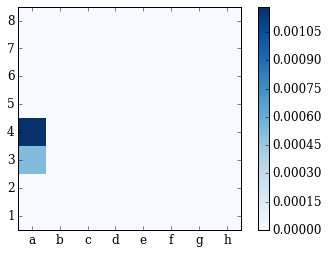
\includegraphics[width=\textwidth]{img/best_moves/output_14_0.png}
%         \caption{$P_{\textsc{pawn}}(B, a_2)$}
%         \label{figure:initialboardc}
% %         {Predicted probability distribution\\
% %         for the ``to'' position\\
% %         for a2 pawn.}
%     \end{subfigure}%
%     ~ 
%     \begin{subfigure}[t]{0.5\textwidth}
%         \centering
%         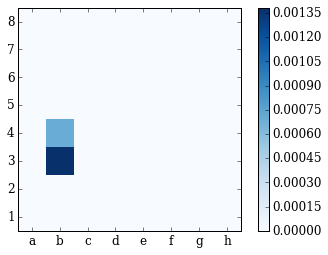
\includegraphics[width=\textwidth]{img/best_moves/output_14_1.png}
%         \caption{$P_{\textsc{pawn}}(B, b_2)$}
% %         \caption{Predicted probability distribution\\
% %         for the ``to'' position\\
% %         for b2 pawn.}
%     \end{subfigure}
%     ~
%     \begin{subfigure}[t]{0.5\textwidth}
%         \centering
%         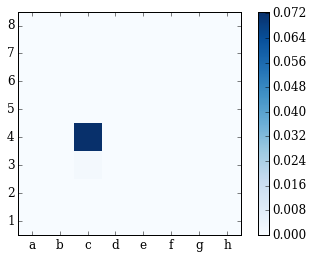
\includegraphics[width=\textwidth]{img/best_moves/output_14_2.png}
%         \caption{$P_{\textsc{pawn}}(B, c_2)$}
% %         \caption{Predicted probability distribution\\
% %         for the ``to'' position\\
% %         for c2 pawn.}
%     \end{subfigure}%
%     ~
%     \begin{subfigure}[t]{0.5\textwidth}
%         \centering
%         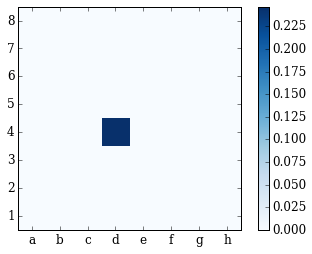
\includegraphics[width=\textwidth]{img/best_moves/output_14_3.png}
%         \caption{$P_{\textsc{pawn}}(B, d_2)$}
% %         \caption{Predicted probability distribution\\
% %         for the ``to'' position\\
% %         for d2 pawn.}
%     \end{subfigure}
% \end{figure}
% \begin{figure}[H]
%   \ContinuedFloat
%     \begin{subfigure}[t]{0.5\textwidth}
%         \centering
%         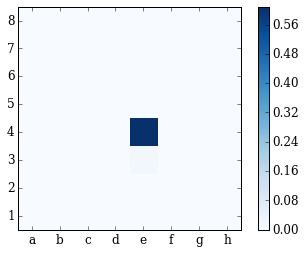
\includegraphics[width=\textwidth]{img/best_moves/output_14_4.png}
%         \caption{$P_{\textsc{pawn}}(B, e_2)$}
%     \end{subfigure}%
%     ~ 
%     \begin{subfigure}[t]{0.5\textwidth}
%         \centering
%         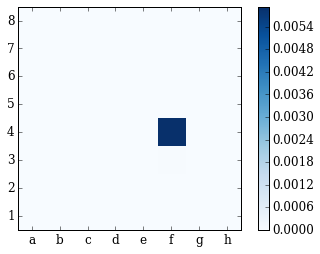
\includegraphics[width=\textwidth]{img/best_moves/output_14_5.png}
%         \caption{$P_{\textsc{pawn}}(B, f_2)$}
%     \end{subfigure}
%   ~
%     \centering
%     \begin{subfigure}[t]{0.5\textwidth}
%         \centering
%         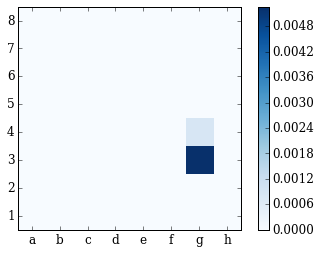
\includegraphics[width=\textwidth]{img/best_moves/output_14_6.png}
%         \caption{$P_{\textsc{pawn}}(B, g_2)$}
%     \end{subfigure}%
%     ~ 
%     \begin{subfigure}[t]{0.5\textwidth}
%         \centering
%         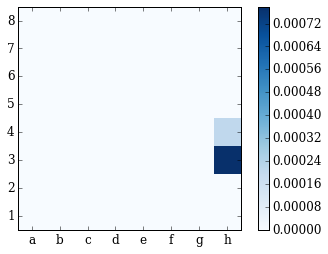
\includegraphics[width=\textwidth]{img/best_moves/output_14_7.png}
%         \caption{$P_{\textsc{pawn}}(B, h_2)$}
%     \end{subfigure}
%     ~
%     \begin{subfigure}[t]{0.5\textwidth}
%         \centering
%         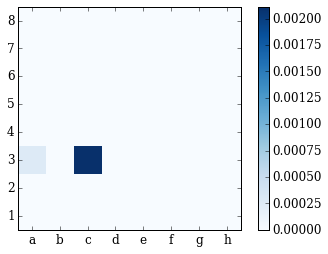
\includegraphics[width=\textwidth]{img/best_moves/output_14_8.png}
%         \caption{$P_{\textsc{knight}}(B, b_1)$}
%     \end{subfigure}%
%     ~ 
%     \begin{subfigure}[t]{0.5\textwidth}
%         \centering
%         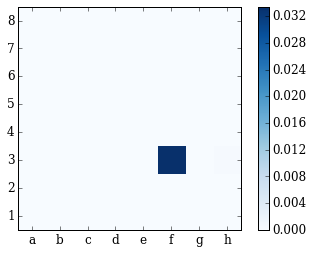
\includegraphics[width=\textwidth]{img/best_moves/output_14_9.png}
%         \caption{$P_{\textsc{knight}}(B, g_1)$}
%         \label{figure:initialboardl}
%     \end{subfigure}
%     \caption[Predictions for initial board position]{
%     (a) The initial board position for a chess game, 
%     (b) The predicted probability distribution for the ``from'' piece by the 
% \textsc{PIECE} network, 
%     (c)-(j) The predicted probability distributions for the ``to'' position by 
% the \textsc{PAWN} network for a2 to h2, 
%     (k)-(l) The predicted probability distribution for the ``to'' position by 
% the \textsc{KNIGHT} network for b1 and g1 respectively.}
% \label{figure:initialboard}
% \end{figure}


\subsection{Checkmating}
In figure \ref{figure:checkmating}, there is a checkmate possible in one move. 
We observe that the most probable move output by our model actually wins it for 
the white player.
\begin{figure}[H]
\hspace*{-0.5in}  
  \centering
    \begin{subfigure}[t]{\textwidth}
        \centering
        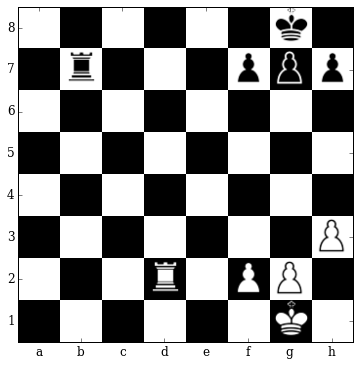
\includegraphics[scale=0.75]{img/best_moves/output_21_0.png}
        \caption{Board position. There is a check and mate 
possible in one move of the white.}
    \end{subfigure}%

 \hspace*{-0.5in}  
    \begin{subfigure}[t]{0.5\textwidth}
        \centering
        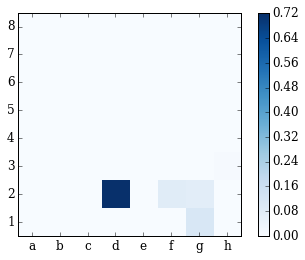
\includegraphics[width=\textwidth]{img/best_moves/output_21_2.png}
        \caption{$P_{\textsc{piece}}(B)$}
    \end{subfigure}
    ~
    \begin{subfigure}[t]{0.5\textwidth}
        \centering
        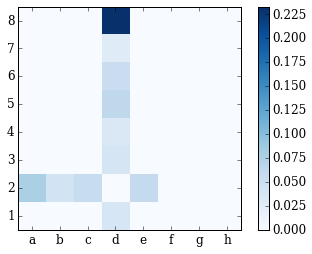
\includegraphics[width=\textwidth]{img/best_moves/output_21_6.png}
        \caption{$P_{\textsc{rook}}(B, d2)$}
    \end{subfigure}%
    \caption{Predictions for a checkmate-in-1 position}
\small
\justifying
(a) Black king is trapped in the last row. Moving the white rook 
at d2 to d8 will win the game for white. (b) The \textsc{PIECE} network 
predicts moving the rook at d2 with $p=0.72$. (c) The \textsc{ROOK} network 
predicts moving the rook to d8 with a total probability of $p=0.225$.

\label{figure:checkmating}
\end{figure}

\subsection{Detecting a check and blocking a promotion}
In figure \ref{figure:check-detection}, the king is under attack by the pawn, 
which is also seeking a promotion in the next move if the king moves away. The 
model successfully that the king should prevent the check by making the 
move \textbf{g1h1} which eventually also prevents the pawn promotion.

\begin{figure}[H]
\hspace*{-0.5in}  
  \centering
    \begin{subfigure}[t]{\textwidth}
        \centering
        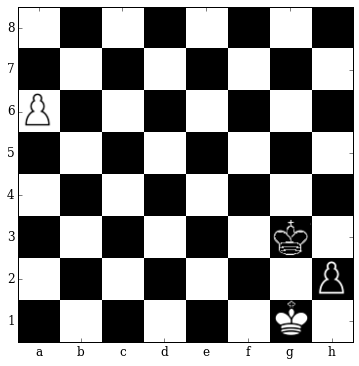
\includegraphics[scale=0.65]{img/best_moves/output_24_0.png}
        \caption{Board position. The white king is under check.}
    \end{subfigure}%

 \hspace*{-0.5in}  
    \begin{subfigure}[t]{0.5\textwidth}
        \centering
        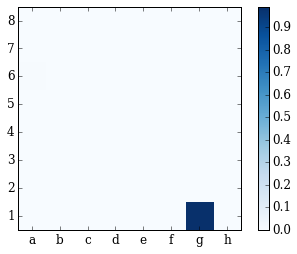
\includegraphics[width=\textwidth]{img/best_moves/output_24_2.png}
        \caption{$P_{\textsc{piece}}(B)$}
    \end{subfigure}
    ~
  \centering
    \begin{subfigure}[t]{0.5\textwidth}
        \centering
        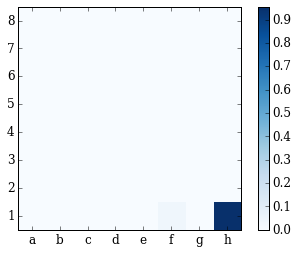
\includegraphics[width=\textwidth]{img/best_moves/output_24_6.png}
        \caption{$P_{\textsc{king}}(B, g1)$}
    \end{subfigure}%
    \caption{Prediction: Detecting a check}
    \small
    \justifying
    (a) White king is under a check. The black pawn at h2 is 
also looking for promotion in the next move. (b) The \textsc{PIECE} network 
predicts moving the king at g1 with $p>0.95$. (c) The \textsc{KING} network 
predicts moving the white king to h1 with a total probability of $p>0.9$.
\label{figure:check-detection}
\end{figure}

\subsection{En passant Move}
A very striking observation in our experiments was the the prediction of an 
en-passant move. It is interesting to note that an en-passant move is a very 
special case of  pawn movement and attack, and we might expect it to appear 
only a very few number of times in our training dataset. However, its 
effectiveness is properly captured by the ensemble of piece and move selector 
networks.
\begin{figure}[H]
\hspace*{-0.5in}  
  \centering
    \begin{subfigure}[t]{\textwidth}
        \centering
        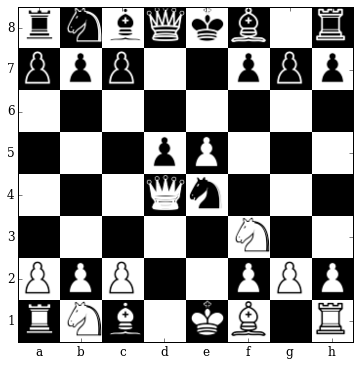
\includegraphics[scale=0.65]{img/best_moves/output_38_0.png}
        \caption{Board position. The d-pawn just moved 2 steps. En passant is 
possible}
    \end{subfigure}%

 \hspace*{-0.5in}  
    \begin{subfigure}[t]{0.5\textwidth}
        \centering
        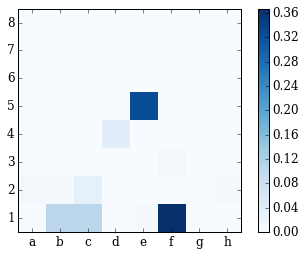
\includegraphics[width=\textwidth]{img/best_moves/output_38_2.png}
        \caption{$P_{\textsc{piece}}(B)$}
    \end{subfigure}
    ~
  \centering
    \begin{subfigure}[t]{0.5\textwidth}
        \centering
        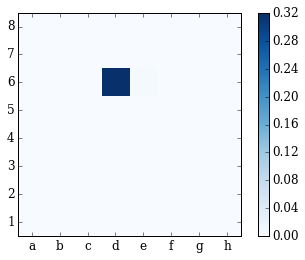
\includegraphics[width=\textwidth]{img/best_moves/output_38_6.png}
        \caption{$P_{\textsc{pawn}}(B, e5)$}
    \end{subfigure}%
    \caption{Prediction: En passant move}
    \small
    \justifying
    (a) An en-passant move is possible. (b) The maximum probable piece to move 
is the e5 pawn. (c) Unmasked probability has the en-passant move as the most 
probable move. During gameplay, if the black didn't move two steps in the last 
move, we can mask out this probability.
\label{figure:enpassant}
\end{figure}

\subsection{Castling}
In figure \ref{figure:castling} below, a castling move is predicted as the most 
favorable move.

\begin{figure}[H]
\hspace*{-0.5in}  
  \centering
    \begin{subfigure}[t]{\textwidth}
        \centering
        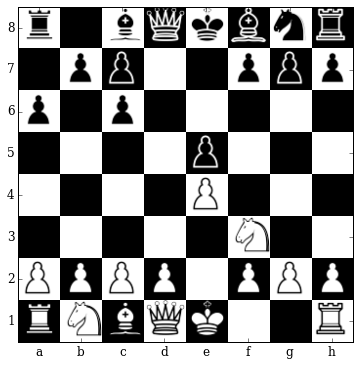
\includegraphics[scale=0.65]{img/best_moves/output_22_0.png}
        \caption{Board position. Castling is one of the favorable moves 
available.}
    \end{subfigure}%

 \hspace*{-0.5in}  
    \begin{subfigure}[t]{0.5\textwidth}
        \centering
        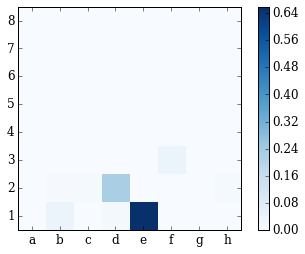
\includegraphics[width=\textwidth]{img/best_moves/output_22_2.png}
        \caption{$P_{\textsc{piece}}(B)$}
    \end{subfigure}
    ~
  \centering
    \begin{subfigure}[t]{0.5\textwidth}
        \centering
        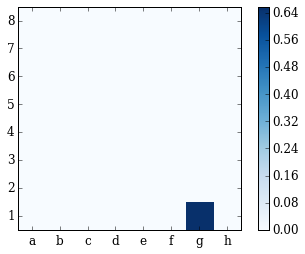
\includegraphics[width=\textwidth]{img/best_moves/output_22_6.png}
        \caption{$P_{\textsc{king}}(B, e1)$}
    \end{subfigure}%
    \caption{Prediction: Castling move}
    \small
    \justifying
    (a) Castling is available for the current board position (b) The 
\textsc{Piece} network predicts moving the king at e1 with $p>0.64$. (c) The 
\textsc{King} network predicts moving the white king to g1 with a total 
probability of $p>0.64$ completing the castling move.
\label{figure:castling}
\end{figure}

\vfill
\subsection{Middle game behavior}
Playing a move using the first guess is not ideal in a middlegame situation. 
Most of the players try to adopt tactics and long term strategies. However, our 
network trained on just 1 step outputs, may not be aware of such strategies. 
But, it is worth observing the behavior of our model when it comes to blunders 
by the opponents and we can take advantage of it.

We present here a game between Magnus Carlsen (white) and Viswanathan Anand 
(black), where Carlsen made a mistake at the 26th move while he easily had a 
good control of the game. Anand oversaw the better move Nex5! to play a4?. Anand 
later realized his mistake, but it was too late and Carlsen had already regained 
the control over the board.\\

We make our model predict the moves Vishwanathan 
Anand should have played after Carlsen's blunder. It is worth noting that the 
most favorable move as suggested by experts was Nex5 (i.e. g6e5), while Anand 
played a4 (i.e. a5a4). Our model predicts that the more favorable move be played 
with a much higher probability (around 6 times) than the actual move. Since 
it is not the best ranked move in our model's prediction, this also 
demonstrates the need to use search along with a prediction model to play a 
better game especially during the middle games. \\

The commentary is available at: \\
\url{http://en.chessbase.com/post/sochi-g6-carlsen-won-anand-missed-big-chance}
Most of the commentators following the game called Anand's move 26 a missed 
opportunity. A tweet said-- \textit{``Wow 26...Ne5! and black is 
winning....Anand plays 26...a4? Whats going on :) \#CarlsenAnand''}

\begin{figure}[H]
\hspace*{-0.5in}  
  \centering
  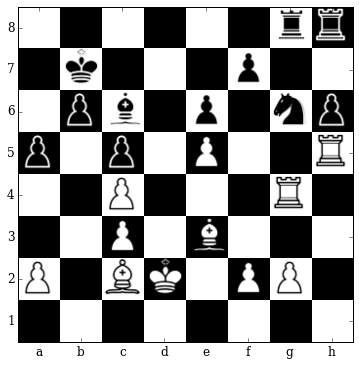
\includegraphics[scale=0.65]{img/best_moves/vishy-magnus.png}
  \caption[Middle game case study]{Black to move. 26th move. 6th game of 
the World Championship match, 2014-- Magnus Carlsen vs Viswanathan Anand}

\label{figure:carlsen-vs-vishy}
\end{figure}

\begin{table}[H]
\centering
\begin{tabular}{@{}lll@{}}
\cmidrule(r){1-2}
Move & Predicted Probability &                                  \\ 
\cmidrule(r){1-2}
g8d8 & 0.252880722284        &                                  \\
g8g7 & 0.148237019777        &                                  \\
g6e5 & 0.13111974299         & Expected Move                    \\
b7c7 & 0.0660261586308       &                                  \\
h8h7 & 0.0471959412098       &                                  \\
c6g2 & 0.0403394699097       &                                  \\
c6e8 & 0.0358173549175       &                                  \\
g8c8 & 0.0323895104229       &                                  \\
b7c8 & 0.0302288047969       &                                  \\
c6d7 & 0.0250529013574       &                                  \\
a5a4 & 0.0231475103647       & Vishwanathan Anand's actual move \\
g6e7 & 0.0229441132396       &                                  \\
b7a6 & 0.0208601523191       &                                  \\
g8a8 & 0.0198916308582       &                                  \\
b7b8 & 0.0190593209118       &                                  \\
c6a4 & 0.0153007712215       &                                  \\
g6f8 & 0.0150824002922       &                                  \\
g8f8 & 0.0115283448249       &                                  \\
g8e8 & 0.00727259740233      &                                  \\
b7a7 & 0.00666899653152      &                                  \\ 
\cmidrule(r){1-2}
\end{tabular}
\caption{Possible moves after the mistake by Carlsen in Move 26}
\label{table:vishy-carlsen}
\end{table}

\section{Board Evaluations}
\label{section:boardevaluations}
In this section we will look at some of the evaluation values 
($V_\gamma(board)$) predicted by the CNN trained to learn an evaluation 
function ($V_\gamma$) as described in chapter \ref{chap:implementation}. For 
each board position, we present boards with the highest evaluation values that 
can be reached from the current board position through a legal move. For 
probity, we also include the moves that might leave or put the king in check, 
but are otherwise valid. We also include legal castling moves.

\begin{figure}[H]
\vspace{-0.2in}
\hspace*{-0.5in}  
  \centering
    \begin{subfigure}[t]{\textwidth}
        \centering
        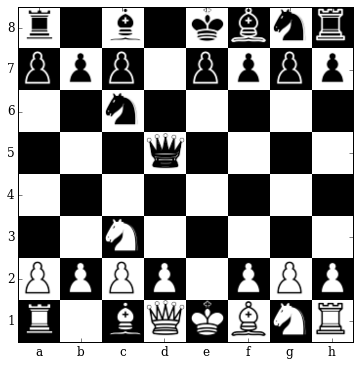
\includegraphics[scale=0.55]{img/table_evaluations/output_11_0.png}
        \caption{Board position (White to move)}
    \end{subfigure}%

 \hspace*{-0.5in}  
    \begin{subfigure}[t]{0.45\textwidth}
        \centering
        
    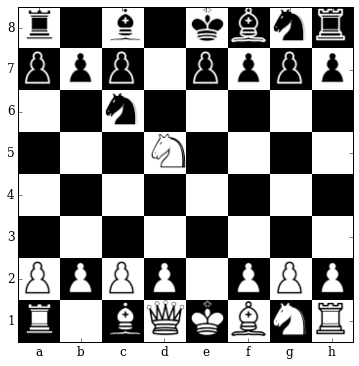
\includegraphics[width=\textwidth]{img/table_evaluations/output_11_2.png}
        \caption{Move: c3d5\\
        $V_{\gamma=0.7}=0.0545$}
    \end{subfigure}
   \hspace{1em}
  \centering
    \begin{subfigure}[t]{0.45\textwidth}
        \centering
        
    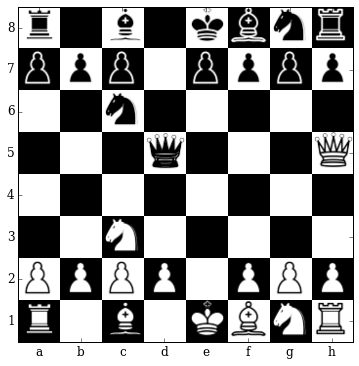
\includegraphics[width=\textwidth]{img/table_evaluations/output_11_4.png}
        \caption{Move: d1h5\\
        $V_{\gamma=0.7}=0.0144$}
    \end{subfigure}
    \caption{Evaluation function: Capturing a Queen with a knight}
    \small
    \justifying
(a) Black has made a mistake by moving the queen to an open position where 
it is under attack from a white knight; (b)-(c) The top two evaluated boards 
reachable from the current position through a legal move.
\label{figure:eval:queen-capture}
\end{figure}

\begin{figure}[H]
\vspace{-0.2in}
\hspace*{-0.5in}  
  \centering
    \begin{subfigure}[t]{\textwidth}
        \centering
        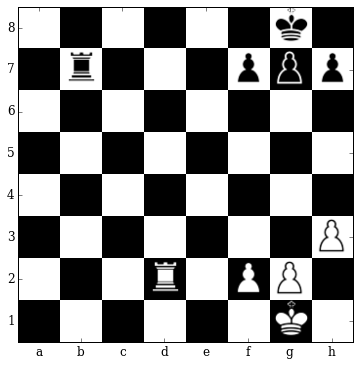
\includegraphics[scale=0.55]{img/table_evaluations/output_12_0.png}
        \caption{Board position (White to move)}
    \end{subfigure}%

 \hspace*{-0.5in}  
    \begin{subfigure}[t]{0.45\textwidth}
        \centering
        
    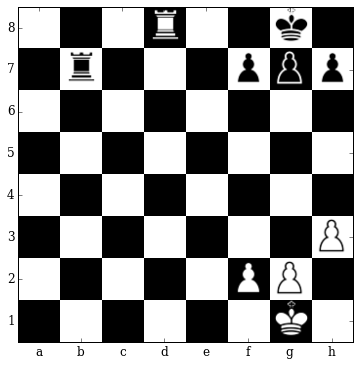
\includegraphics[width=\textwidth]{img/table_evaluations/output_12_2.png}
        \caption{Move: d2a8\\
        $V_{\gamma=0.7}=0.0543$}
    \end{subfigure}
   \hspace{1em}
  \centering
    \begin{subfigure}[t]{0.45\textwidth}
        \centering
        
    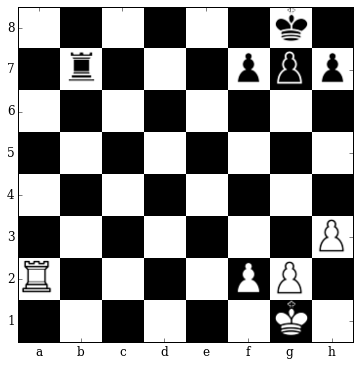
\includegraphics[width=\textwidth]{img/table_evaluations/output_12_4.png}
        \caption{Move: d2a2\\
        $V_{\gamma=0.7}=0.0177$}
    \end{subfigure}
    \caption{Evaluation function: Checkmate in one move}
    \small
    \justifying
    (a) A checkmate is possible in just one move of white; (b) The board with 
highest evaluation score in one move distance from the current board. It is a 
check and a mate. (c) The second best move predicted by the evaluation 
function. The value is less than 0.4 times the highest value.
\label{figure:eval:checkmate}
\end{figure}

\begin{figure}[H]
\vspace{-0.2in}
\hspace*{-0.5in}  
  \centering
    \begin{subfigure}[t]{\textwidth}
        \centering
        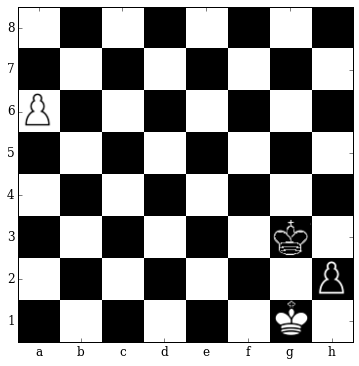
\includegraphics[scale=0.55]{img/table_evaluations/output_15_0.png}
        \caption{Board position (White to move)}
    \end{subfigure}%

 \hspace*{-0.5in}  
    \begin{subfigure}[t]{0.45\textwidth}
        \centering
        
    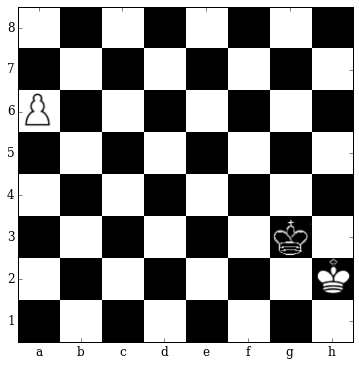
\includegraphics[width=\textwidth]{img/table_evaluations/output_15_2.png}
        \caption{Move: g1h2 \\
        $V_{\gamma=0.7}=0.0216$}
    \end{subfigure}
   \hspace{1em}
  \centering
    \begin{subfigure}[t]{0.45\textwidth}
        \centering
        
    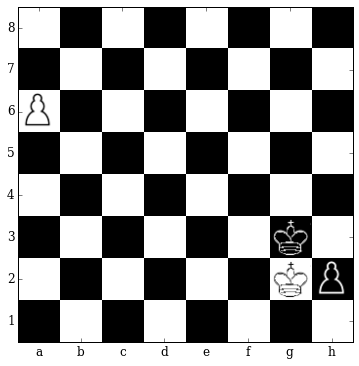
\includegraphics[width=\textwidth]{img/table_evaluations/output_15_4.png}
        \caption{Move: g1g2 \\
        $V_{\gamma=0.7}=0.0084$}
    \end{subfigure}
    \caption{Evaluation function: Check detection and promotion prevention}
    \small
    \justifying
    (a) White to move. The white king is currently under check by the black 
pawn at h2. If the king moves away, the pawn will promote to a queen and can 
wrap up the game easily afterwards; (b) The board with the highest evaluation 
is the one where the king captures the pawn. (c) The board with the second 
highest evaluation is the one where the king puts itself into check.
\label{figure:eval:check-promotion}
\end{figure}

There are a couple of interesting observations that we can make from the few 
examples above:
\begin{enumerate}
 \item \textbf{Piece Capture}
 In figures \ref{figure:eval:queen-capture} and 
\ref{figure:eval:check-promotion}, the boards with highest value in the next 
move have one less opponent piece than the preceding board i.e. a white piece 
captures a black piece. This is not the case in figure 
\ref{figure:eval:checkmate}, probably because there was no direct piece capture 
possible.
 \item \textbf{Board value is analogous to sum of piece values} In most of the 
examples above, %as well as the ones in Appendix
we can observe a similar trend-- the board is evaluated in a way similar to a 
function that computes the difference in the values of the pieces remaining for 
both the players. We will probe further into this observation further in 
\ref{subsection:correlation} where we see the correlation between this and a 
common piece evaluation system.
\end{enumerate}

\subsection{Correlation with the Material heuristic}
\label{subsection:correlation}
To investigate the properties of the evaluation function, we computed the 
correlation of the values given by $V_\gamma(board)$ with the following 
heuristically derived evaluation function ($V_{\textsc{MATERIAL}}(board)$):
\begin{table}[H]
\centering
\begin{tabular}{@{}llllll@{}}
\toprule
{\bf Piece} & Pawn & Rook & Knight  & Bishop & Queen \\ \midrule
{\bf Value} & 1    & 5    & 3	    & 3      & 9     \\ \bottomrule
\end{tabular}
\caption{The most common assignment of piece valuations}
\end{table}
Some variations value the king highly, we do not use any such assignment 
because kings are present for both the players during the whole course of the 
game and hence won't impact our evaluation as such.\\

So the function $V_{\textsc{MATERIAL}}$ is as follows:\\
$V_{\textsc{MATERIAL}}(board) = 1 \times (P-P') + 3 \times (N-N')+ 3 \times 
(B-B') + 5 
\times (R-R')+ 9 \times (Q-Q')$\\
\hspace{0.25in}where $P, N, B, R, Q$ represent the number of pawns, knights, 
bishops, rook, queen respectively for the white player and $P', N', B', R', Q'$ 
refer to their black counterparts.\\

The value of Pearson's correlation coefficient\footnote{Pearson's 
correlation coefficient ($\rho$) between two random variables is also 
referred to as the \textit{product moment} i.e. the mean of the product of the 
adjusted random variables. It can be computed using the formula: $\rho = 
\frac{E[(X-\mu_X)(Y-\mu_Y)]}{\sigma_X\sigma_Y}$
} we obtain for a set of $665,727$ boards between evaluation done with the 
model 
$V_{\gamma=0.7}$ and $V_{\textsc{MATERIAL}}$ is \textbf{0.8194}. 
Figure~\ref{figure:correlation} plots the evaluation function values for two 
functions 
for different boards. The correlation seems evident from the scatter plot. We 
also consider some example boards in figure~\ref{figure:correlation2}. The 
boards with a positive material value for white have a positive evaluation in 
our function. It is worth noting that in figure~\ref{figure:correlation2d}, 
white has almost won and it has a board value of 20 and an evaluation function 
suggests that white is approximately 3 moves away from winning ($(0.7)^3 = 
0.34$).\\

\begin{figure}[H]
 \includegraphics[scale=0.75]{plots/correlation_eval.pdf}
 \caption[Correlation between $V_{\gamma=0.7}$ and 
$V_{\textsc{MATERIAL}}$]{Scatter plot showing $V_{\gamma=0.7}$ and 
$V_{\textsc{MATERIAL}}$ values for different boards in the test dataset}
\label{figure:correlation}
\end{figure}

\begin{figure}[h]
\vspace{-0.2in}
\hspace*{-0.5in}  
  \centering
    \begin{subfigure}[t]{0.45\textwidth}
        \centering
        \includegraphics[scale=0.55]{img/table_evaluations/output_35_0.png}
        \centering
        \caption{$V_{\gamma=0.7} = 0.0015796$\\  
$V_{\textsc{MATERIAL}}= 0.0 $}
  \label{figure:correlation2d}
    \end{subfigure}%
    \hspace{1em}
    \begin{subfigure}[t]{0.45\textwidth}
        \centering
        \includegraphics[scale=0.55]{img/table_evaluations/output_33_0.png}
         \caption{$V_{\gamma=0.7} = -0.0748723$\\  
$V_{\textsc{MATERIAL}}= -6.0 $}
    \end{subfigure}%

 \hspace*{-0.5in}  
    \begin{subfigure}[t]{0.45\textwidth}
        \centering
        
    \includegraphics[width=\textwidth]{img/table_evaluations/output_34_0.png}
         \caption{$V_{\gamma=0.7} = 0.0902274$\\  
$V_{\textsc{MATERIAL}}= 2.0 $}
    \end{subfigure}
   \hspace{1em}
  \centering
    \begin{subfigure}[t]{0.45\textwidth}
        \centering
        
    \includegraphics[width=\textwidth]{img/table_evaluations/output_36_0.png}
         \caption{$V_{\gamma=0.7} = 0.302926$\\  
$V_{\textsc{MATERIAL}}= 20.0 $}
    \label{figure:correlation2d}
    \end{subfigure}
    \caption{Comparing the evaluation functions $V_{\gamma=0.7}$ and 
$V_{\textsc{MATERIAL}}$ }
\label{figure:correlation2}
\end{figure}


While a correlation coefficient of 0.8194 is pretty impressive, it doesn't 
actually imply a good evaluation function. Rather it provides a significant 
evidence of the nature of the evaluation function learned by our CNN based 
architecture without any prior knowledge of the importance of pieces or even any 
knowledge of the rules. The difference however is that the CNN based evaluation 
function is much more complex and makes use of shared weights to score local 
patterns to evaluate the complete board. This is what motivated to solve a 
regression problem using a convolutional neural network.\\

Although there are significant variations to the basic evaluation scheme we 
compare here, like the ones that score single pieces or pairs of pieces on the 
basis of its rank and file and/or the number of liberties, we omit comparing 
our evaluation function against them since our aim was just to present a idea of 
the similarity between such a set of hand-crafted heuristically defined 
evaluation functions.

\subsection{Game Trajectories}
\begin{figure}[H]
  \hspace*{-1.0in}
 \includegraphics[width=1.5\textwidth]{plots/board_evals_win.pdf}
 \caption[Game Trajectories]{t-SNE embedding of the activations at the last 
fully connected layer of the board evaluation CNN. The red end is the set of 
boards close to winning, the blue end is the set of boards close to losing 
a game. We plot a game on the embedding. The winner(yellow) ends on the red 
side of the embedding while the loser(cyan) ends on the blue side of the 
embedding}
\end{figure}
\label{subsection:trajectories}
As an analysis to the evaluation function proposed, we tried to observe the 
evaluations of the boards observed in a few test set games. In 
figure~\ref{figure:gametrajectory}, the scatter plot shows a set of $10,000$ 
boards from our test dataset embedded onto a two dimensional embedding of 
the activations caused at the last fully connected layer of the board 
evaluation CNN using t-SNE~\cite{tsne}. The game trajectories i.e. the path of 
the boards as seen on the two dimensional embedding for both the winning and 
the losing players is shown on the plot. A description of the game could be that 
the two players had boards with similar evaluation before one of them starts to 
win i.e. gets to see boards with higher positive evaluation values.\\




\section{Gameplay}
In this section we describe and discuss how well our models do when playing 
against a computer. It needs to be emphasized again that the primary 
motivation of our work is not the build the strongest chess playing 
system, but to show as a proof of concept that the convolutional neural 
network architecture can indeed learn how to play chess and also make strong 
predictions. \\
We already demonstrated the strengths and weaknesses of both our 
models on various cases in a game of chess. Since the actual gameplay is 
tougher than solving individual cases even with high accuracy, we may expect our 
system to make blunders which makes it lose matches. It is apparent that a 
heuristic search with a large amount of chess knowledge can help make the system 
robust to blunders.\\

Since our entire source code is in \textit{Python}, we wanted to choose a 
Python based chess playing system which was easy to integrate with our 
prediction and evaluation system rather than be in an arms race with the best 
systems like Rybka \cite{wiki:rybka} and Stockfish, which use optimizations and 
tweaks upto 
the level of memory addresses and assembly code generation. We went for Sunfish 
\cite{sunfish}, which is a short and lucid python chess program which implements 
MTD-f for search. We also utilize the API like structure of Sunfish to inject 
the minimal chess knowledge required for our system and hence play the predicted 
moves.\\

\begin{table}[width=1.5\textwidth]
\centering
\hspace*{-1.0in}
\begin{tabular}{@{}llllll@{}}
\toprule
{\bf Method Used} & Games Played & Won & Drawn & Lost & 
Details                      \\ \midrule
Top-Prob          & 73           & 7         & 20          & 46         & 
$10\leq maxn\leq 1000$ \\\\
TopProb-Negamax&19     &3        &4		   & 12           & 
$10\leq maxn\leq 100$ \\\\
Evaluation function ($V_{\gamma=0.7}$)&&&&&\\
with Negamax &   21      & 6  &   4           & 11       &  2 \textless Negamax 
depth \textless 5 \\\\
Evaluation function ($V_{\gamma=0.7}$)&&&&&\\
with Negamax& 25        &  16 & 2             & 7       & Negamax depth=4       
                      \\\\
%                   &              &           &             &            &        
%                       \\
%                   &              &           &             &            &        
%                       \\
%                   &              &           &             &            &        
%                       \\ 
                      \bottomrule
\end{tabular}
\hspace*{-1.2in}
\caption[Results against negamax]{The table shows the result statistics for 
evaluation of gameplay against sunfish. We test our models under different 
conditions. In most of our experiments we limit the number of nodes explored by 
Sunfish between 10 to 1000 (chosen randomly on a log scale). For other 
deviations, the details are mentioned in the details column}
\label{table:gameplay}
\end{table}

The fact that our models do not perform well against Sunfish, that too with 
limited search capability, is not disheartening. Looking at the implementations 
of some of the best-known chess computers with all the bitmap optimizations 
and computations, we believe that there is still a long way in a Convolutional 
neural network becoming the primary backend of such a system. As we already 
emphasized enough, that the aim of our work has never been to be in an arms 
race with the best known chess computers around, but to provide a proof of 
evidence that convolutional neural networks can indeed play a game of chess.\\

It is worth mentioning that examples like the model learning to predict only 
the legal moves at any board position is a strong result in itself. Further, 
the analysis shown earlier in the chapter (sections~\ref{section:samplemoves}, 
\ref{section:boardevaluations}) shows positive outcomes for even some of the 
tricky cases. Also, during the gameplay it was observed that a proper pawn 
structure, castling move and defense for the king were prominent features of 
most of the games. This strengthens the evidence this work provides in 
human-like chess players with generalization and pattern recognition capability. 
 We discuss about these strengths, possible reasons for the weaknesses and 
propose extensions of this work in the next chapter.

% \subsection{}
% Since the individual networks have to predict from a set of size 64, the 
% evaluation cannot be made with respect to the actual move which comes from a 
% set of $64\times 64$. Hence, we evaluate predictions as the games in our test 
% dataset proceed.  
% 
% \begin{figure}
% \includegraphics[width=1.5\textwidth,center]{plots/accuracy-move_num2.pdf}
% \caption{Accuracy vs Move number}
% \label{figure:gameplay1}
% \end{figure}
% \begin{figure}
% \includegraphics[width=1.5\textwidth,center]{plots/hitrate.pdf}
% \caption{Legal Move rate vs Move Number}
% \label{figure:gameplay2}
% \end{figure}
% \begin{figure}
%   \includegraphics[width=1.5\textwidth,center]{plots/accuracies@k.pdf}
%   \caption{Curves}
%   \label{figure:p}
% \end{figure}%the most important section...Still the worst/no results :(

	\chapter{Conclusion and Discussion}

We started with an aim to make a machine learn how to play chess giving it no 
or minimal prior knowledge. In the previous chapter, we saw a mannerly analysis 
of the results we obtain when convolutional neural networks are used to learn 
the game of chess. Although showing a promising behavior in various case 
studies performed, we saw that the gameplay is not very effective against a 
decent chess computer that uses heuristic search to choose a move. But, we 
believe that the work significantly bridges the gap between the cognitive 
aspects of chess playing and how the best chess computers play it. In this 
chapter, we discuss the contributions of our work and alongside try to 
ponder upon the shortcomings and discussing possible solutions.\\

\section{Positives}
We started with a motive to make a machine learn the game of chess with minimal 
prior knowledge and eventually have the ability to:
\begin{itemize}
 \item Learn to play legal moves
 \item Rank the possible moves without any explicit guidance on relative 
importance of material or position
 \item Evaluate board positions
\end{itemize}

Motivated to accomplish this task using minimal knowledge prior, we used 
convolutional neural network based architectures to learn-- the piece and move 
predictors as well as an evaluator. In the last section, we empirically 
demonstrated that the models learned the rules of the chess as well were able 
to make strong predictions on tasks where a novice could easily fail.



\section{Weaknesses}
We have already emphasized that our motivation was not to build a state of the 
art chess playing system, but to build a chess player from 
scratch i.e. having minimal prior knowledge. We saw in the last chapter that 
the gameplay of our system is not a championship level one. But it still could 
make strong predictions on certain tasks. However in this section, we will try 
to focus on the weaknesses of our models.\\

\subsection{Reasons}
The convolutional neural network trained on all the moves doesn't know if the 
given move at hand is a blunder or not. It can be the case that a common 
blunder is mistaken to be a favorable move in certain situations or if a board 
position is so rare that the only available supervision is not the best move to 
make in that situation.\\

However this can be explained to be considered while learning the evaluation 
function using discounted rewards. The problem with the evaluation function 
seems to be that the learning task is not very specific or well formulated. A 
visible weakness is the already present ambiguity in the training data for the 
network for instance the starting board, which looks the same for both the 
winning and the losing player, gets both a positive and a negative score. 
Although the value is small or can be made making a proper use of the decay 
parameter. 

\section{Further Work}
\subsection{Reinforcement Learning based player}
In chapter~\ref{chap:introduction}, we mentioned that it is a hard problem 
to 
do a policy search using a reinforcement learning architecture when we have a 
combination of complex dynamics and complex policy. Intuitively, why a 
reinforcement learning agent (RL agent) is a bad idea for chess is that a 
reward is received only once and after a long time. Hence, a learner who starts 
from scratch, using a random policy, would never reach the point when it 
receives a positive reward i.e. a win. There has to be a heuristic evaluation of 
the policy learned by such a system which allows it to update its policy. It is 
exactly at this point where the evaluation function learned from a large 
dataset of already played games can fit. The evaluation function (described 
in~\ref{section:eval-func}) computed at a certain ply depth can provide the 
board values as a feedback to the 
current policy of the RL agent.

\subsection{Evolving chess programs using Genetic Algorithms}
Another class of systems that use co-evolution, where the system learn by 
playing itself 
\cite{vazquez-coello-12_evolutionary_hooke-jeeves-algo_chess-evaluation}  and 
adjusting the parameters 
\cite{bovskovic-brest-11_tuning-chess-evaluation-w-differential-evolution}. A 
possible extension of this work could be to utilize such genetic programming 
architectures to improve the basic piece-move predictor presented in this 
thesis.


\section{Conclusion}
Through our work, we presented a novel proof of evidence that cognitively 
inspired architectures rather than the conventional chess playing systems can 
also be used to build chess systems. Such chess systems have a more human way 
of playing chess and do not require much knowledge about the rules of chess 
too. We demonstrated the strengths and weaknesses of our work and discussed 
some extensions which could lead to better chess playing systems in the future.
	
	\backrefsetup{disable}
%	\appendix 
%	\chapter{Development Details}

%	\section{Last.FM APIs}
%		An api-key is required for calling the api. This can be obtained by creating a developer account on their website.
		
%		Base URL: http://ws.audioscrobbler.com
%\begin{itemize}
%	\item Recent Tracks: URL: /2.0/?method=user.getrecenttracks\&user=<user>\&api\_key=<api\_key>\&format=<format>
%		<user>: The user for which the history is to be fetched.
%		<api\_key>: Obtained from their developer's portal.
%	\item Top Tags: 
%\end{itemize}
	\thispagestyle{empty}
	\cleardoublepage
	\phantomsection
	\backmatter
	\singlespacing
	
	\addcontentsline{toc}{chapter}{Bibliography}
	\bibliographystyle{apalike}
	\bibliography{references}
	
% 	\begin{appendices}
% 	 \chapter{Background}
\label{chap:background}
In this chapter, we will first look at what it means to actually solve the game 
of chess, before moving on to studying how computers are programmed to play 
chess efficiently and exceptionally well. Further we look at some background 
about reinforcement learning, deep learning and 
learning representations and how 
convolutional neural networks, a specific case of deep learning architectures, 
has shaped the field of artificial intelligence especially in the area of 
pattern recognition.% in~\ref{subsection:cnn-background}. 
% In section~\ref{subsection:previous-works}, we also introduce some effective 
% approaches that solve problems similar to the task at hand like playing Atari 
% games using deep reinforcement learning, predicting moves in the games of Go and 
% evaluating moves in chess.  
\section*{Solving Chess}
\label{section:solving}
Solving chess refers to finding an optimal strategy for playing chess. Chess has 
a finite number of states, estimated to be around $10^{43}$ 
by \citet{shannon1950xxii}. \citet{zermelo1913anwendung} proved that a 
hypothetically determinable optimal strategy does exist for chess.\\
In a weaker sense, each position can be assigned as a win for white, a win for 
Black or a forced draw if both the players are using the optimal strategy. We 
can formulate this as a function $f$ for each board position using the procedure 
below.
\begin{enumerate}
\item Assign all the positions with no further play possible as:
\[f(position) = \begin{cases}
1 \text{ , if White has won}\\
0 \text{ , if it is a draw}\\
-1 \text{ , if Black has won}
\end{cases}\]
\item Use the recursive rule up the game tree:
\[f(p) = \max\limits_{p\rightarrow p'} (-f(p'))\]
where $p'$ is a position reachable in one move from position $p$.\\
Here the negative sign means that a win for the opponent is a loss for the 
player in consideration and vice-versa.
\end{enumerate} 
The above recursive rule is the same as the minimax algorithm for the case when 
the game tree for chess is fully grown. The function $f$ gives us the 
``perfect'' evaluation function to play a chess game. While playing the game, we 
just need to choose the move which takes us to the board position $p$ for which 
$f(p)=1$.\\

But this evaluation function, $f$, cannot be computed with the computing 
resources available as of now. Hence, we need to resort to approximations of 
$f(p)$.


\section*{Playing Chess using Computers}
\label{section:playing-background}
The first study on computers playing the game of chess was done by 
\citet{shannon1950xxii}. He predicted two main search strategies that would 
evolve with computers being programmed to play chess--
\begin{enumerate}
\item ``Type A" programs would use a ``brute force" examination of all the board 
positions possible through valid moves upto a certain depth of play.
\item ``Type B" programs would employ a ``quiescence search" looking at only a 
few good moves for each position. 
\end{enumerate}
He also predicted the ``Type A" programs to be impractical because of the 
massive search space. For even a computer evaluating $10^6$ moves per second, a 
lookahead of 3 moves for both sides, when an average of 30 moves are available 
for each board position, the program would take around 13 minutes.\\
\begin{table}[h]
\centering
%\resizebox{\textwidth}{!}
\caption{Time taken to explore 30 moves per position at $10^6$ moves per 
second.}
\label{table:time-taken}
\end{table}

However, with the exponential increase in the computation power since then, the 
most successful methods for playing chess are programmed to use ``Type A" 
programs. One reason for ignoring ``Type B'' is that relying on the board 
configuration to decide on the moves to explore is a much harder problem than 
using a faster, yet weaker, evaluation metric for a larger depth. It is widely 
believed that a faster evaluation function with an efficient search along with 
heuristic pruning would build a better chess playing computer than the one that 
uses a better but slower evaluation function that involves pattern recognition 
techniques similar to our brain.

\subsection*{Conventional Chess Playing Computers}
\label{subsection:conventional-chess}
The fundamental implementation details of chess-playing computer system include:
\begin{itemize}
\item \textbf{Board Representation} -- how a board position is represented in a 
data structure. The performance of move generation and piece evaluation depends 
on the data structure used to represent the board position. The most common 
representation uses a list of piece positions for each position. Some of the 
other methods are-- mailbox, 0x88, bitboards and huffman codes. We will discuss 
the representation used for our training and playing tasks in Chapter 
\ref{chap:dataset}.

\item \textbf{Search Techniques} -- how to identify and select the moves for 
further evaluation. Some of the most widely used search techniques are-- 
Minmax, Negamax, Negascout, Iterative deepening depth-first search etc. Much of 
the 
focus on state of the art chess playing systems resides on making search more 
efficient to evaluate more board positions per unit time. One of these 
algorithms which we make use of is Negamax algorithm and has 
been explained in section~\ref{subsection:interleaved}.

\item\textbf{Leaf Evaluation} -- how to evaluate the position of the board if 
no 
further evaluation needs to be done. The mapping from a board to an integer 
value is called the evaluation function. An evaluation function typically 
considers material value along with other factors affecting the strength of 
play for each player. The most common values for materials is 1 point for pawn, 
3 for bishop, 3 for knight, 5 for rook, 9 for queen and 200 for king. The high 
value for king ensures that checkmate outweighs everything. The sum of the 
values for all material on the board with negative weights to the opponent is 
the evaluation of the table. In addition to pieces, most evaluation functions 
take into consideration more factors like pawn structure, pair of bishops, 
protection of the king etc.
\end{itemize}


\section*{Reinforcement Learning}
\label{section:RL}
The fundamental principle behind all Reinforcement learning methods is that we 
use the current policy, run it on the environment, observe the feedback and 
make the good outcomes more likely, the bad outcomes less likely. Reinforcement 
learning differs from standard supervised learning in the way that an RL 
algorithm is not presented with optimal actions to input states 
\cite{sutton1998reinforcement}. The basic reinforcement learning model contains 
the following components:
\begin{enumerate}
 \item a set of environment states $\mathcal{S}$
 \item a set of actions $\mathcal{A}$
 \item transition rules between states
 \item rules that determine the \textit{scalar intermediate reward} of a 
transition
\item rules that describe what the agent observes
\end{enumerate}
However it is a very hard problem to do a policy search using a reinforcement 
learning architecture when we have a combination of complex dynamics and 
complex policy. The high dimensionality of such policies doesn't allow 
efficient policy search. However, there have been successful attempts to 
convert these complex dynamics and complex policy domain problems to only a 
complex policy problem by decomposing the policy search into two phases-- 
optimal control and supervised learning \cite{levine2015end}. The end to end 
training for the supervised learning part is done using a function 
approximator, convolutional neural networks in our case, which we will 
discuss in section~\ref{subsection:cnn-background}. 
Other attempts to combine conventional reinforcement learning techniques with 
deep learning to learn optimal control have yielded near human performance on 
tasks like playing Atari video games \cite{deepmind_nips}. The task that 
representation learning architectures like CNNs solve is the problem of 
perception i.e. the feature representation of the states need not be 
composed of hand-crafted features, but can be learned while training.

\section*{Deep Learning}
\label{section:dl-background}
The area of Neural Networks has been inspired by the aim of modeling biological 
neural systems. Although it has diverged from this aim since then, the basic 
computational unit in an artificial neural network still remains a neuron, 
which takes the signal from the axons from other neurons as inputs, 
with dendrites carrying the signal to the nucleus where it gets summed up and 
the neuron is activated if the sum is above some threshold. Such a neuron can 
be represented mathematically as: $f(\sum_i w_ix_i + b)$, where $f$ is the 
activation function, $w_i$ is the weight given to the input from one of its 
dendrites. In other words, a neuron computes the dot product of its weights and 
the inputs, adds the bias and applies an activation function. A mathematical 
model of a neuron is shown in the figure below.
\begin{figure}[H]
\begin{tikzpicture}[
init/.style={
  draw,
  circle,
  inner sep=2pt,
  font=\Huge,
  join = by -latex
},
squa/.style={
  draw,
  inner sep=2pt,
  font=\Large,
  join = by -latex
},
start chain=2,node distance=13mm
]
\node[on chain=2] 
  (x2) {$x_2$};
\node[on chain=2,join=by o-latex] 
  {$w_2$};
\node[on chain=2,init] (sigma) 
  {$\displaystyle\Sigma$};
\node[on chain=2,squa,label=above:{\parbox{2cm}{\centering Activate \\ 
function}}]   
  {$f$};
\node[on chain=2,label=above:Output,join=by -latex] 
  {$y$};
\begin{scope}[start chain=1]
\node[on chain=1] at (0,1.5cm) 
  (x1) {$x_1$};
\node[on chain=1,join=by o-latex] 
  (w1) {$w_1$};
\end{scope}
\begin{scope}[start chain=3]
\node[on chain=3] at (0,-1.5cm) 
  (x3) {$x_3$};
\node[on chain=3,label=below:Weights,join=by o-latex] 
  (w3) {$w_3$};
\end{scope}
\node[label=above:\parbox{2cm}{\centering Bias \\ $b$}] at (sigma|-w1) (b) {};

\draw[-latex] (w1) -- (sigma);
\draw[-latex] (w3) -- (sigma);
\draw[o-latex] (b) -- (sigma);

\draw[decorate,decoration={brace,mirror}] (x1.north west) -- node[left=10pt] 
{Inputs} (x3.south west);
\end{tikzpicture}
\caption{An artificial neuron as a mathematical model}
\end{figure}

Neural networks are the collections of neurons that are connected in an acyclic 
graph. This means that outputs of some set of neurons becomes the input of 
another set of neurons. The most common arrangement is a layered neural network 
with an input and an output layer, along with none or more hidden layers. 
The input layer has number of neurons equal to the input dimension and the 
number of output layer neurons is the dimension of the output. The hidden 
layers can contain different numbers of neurons. A two-layer neural network is 
shown in the figure below. The two-layer here refers to the number of layers 
besides the input layer.
\begin{figure}[H]
\begin{tikzpicture}[
plain/.style={
  draw=none,
  fill=none,
  },
net/.style={
  matrix of nodes,
  nodes={
    draw,
    circle,
    inner sep=10pt
    },
  nodes in empty cells,
  column sep=2cm,
  row sep=-9pt
  },
>=latex
]
\matrix[net] (mat)
{
|[plain]| \parbox{1.3cm}{\centering Input\\layer} & |[plain]| 
\parbox{1.3cm}{\centering Hidden\\layer} & |[plain]| \parbox{1.3cm}{\centering 
Output\\layer} \\
& |[plain]| \\
|[plain]| & \\
& |[plain]| \\
|[plain]| & |[plain]| \\
& & \\
|[plain]| & |[plain]| \\
& |[plain]| \\
|[plain]| & \\
& |[plain]| \\
};
\foreach \ai [count=\mi ]in {2,4,...,10}
  \draw[<-] (mat-\ai-1) -- node[above] {Input \mi} +(-2cm,0);
\foreach \ai in {2,4,...,10}
{\foreach \aii in {3,6,9}
  \draw[->] (mat-\ai-1) -- (mat-\aii-2);
}
\foreach \ai in {3,6,9}
  \draw[->] (mat-\ai-2) -- (mat-6-3);
\draw[->] (mat-6-3) -- node[above] {Ouput} +(2cm,0);
\end{tikzpicture}
\caption{A two layer Artificial Neural network}
\end{figure}

In practice, we model a real valued function using a multi-layer neural 
network. This real valued function, for example, is the one which outputs the 
class value in case of a classification task or a continuous function in case 
of a regression task. In other words, a multi-layer artificial neural 
network defines a family of functions parameterized by the weights of the 
network. By learning the weights of such a network we usually means learning a 
function belonging to this family of functions that best represents the training 
data.

\subsection*{Universal Approximation Properties of Multilayer Perceptrons}
\label{subsection:universal-approx}
We discussed above that a family of functions is represented by a single 
artificial neural network with fixed architecture. It has been proved that 
Neural networks with at least one hidden layer are universal 
approximators \cite{hornik1989multilayer}. This means that given any continuous 
function $f(x)$ and some $\epsilon>0$, a Neural network with one hidden layer 
containing a sufficient number of hidden layer neurons and a suitable choice of 
non-linearity, say represented by $g(x)$, exists such that $\forall x, 
|f(x)-g(x)|<\epsilon$. In other words, we can approximate any given real 
valued continuous function with a two layer Neural network upto a certain 
accuracy.\\

The fact that two layer Neural networks are universal approximators 
is a pretty useless property in the case of machine learning. Neither does it 
tell the number of hidden units required to represent a given function upto the 
desired precision, nor does it promise that it represents a generalized function 
that fits the unseen data. The generalized function is expected to be smooth, 
while the overly precise two-layer network may overfit for the input data and 
not learn a promising representation.

\subsection*{Representation Learning}
We learnt that despite being universal approximators, it may not reasonable to 
approximate a function for a task at hand using two-layer Neural networks 
because of insufficient generalization ability. Meanwhile, a lot of 
experimental evidence from the recent past shows that these functions can be 
learnt to a greater generalization using Neural networks of larger depths 
\cite{bengio-dl-book}. Most of these works involve using a specific class of 
Neural networks architectures, namely Convolutional Neural Networks, which we 
will discuss in section \ref{subsection:cnn-background}. This leads us to 
believe that depth indeed is a useful consideration to make while choosing a 
Neural network architecture to fit data, and it provides the learner's family 
of functions multiple levels of representation and hence making the function 
smoother yielding better generalization. 

\subsection*{Convolutional Neural Networks}
\label{subsection:cnn-background}
Convolutional neural networks, sometimes referred to as Convolutional Networks 
or ConvNets, is a particular architecture of deep neural networks inspired 
by the seminal work by \citet{hubel1963shape} on feedforward processing in 
early visual cortex. The architecture uses hierarchical layers of tiled 
convolutional filters to mimic the effects of receptive fields. These filters 
exploit the local spatial correlations present in the images. In 
practice, these hierarchical layers are alternated with subsampling layers like 
max-pool and a non-linearity map, and further connected to fully connected 
layers just like in other deep learning architectures and the full 
network is trained using back propagation. In short, Convolutional neural 
networks are nothing but neural networks which use convolution instead of 
full matrix multiplications in atleast one of the layers \cite{bengio-dl-book}. 
\\
\begin{figure}[H]
\centering
\begin{tikzpicture}

				\node at (0.5,-0.75){\begin{tabular}{c}input 
image\end{tabular}};
		
				\draw (0,0) -- (1,0) -- (1,1) -- (0,1) -- (0,0);
		
				\node at 
(3,3.25){\begin{tabular}{c}convolutional layer\\with 
non-linearities\end{tabular}};
		
				\draw[fill=black,opacity=0.2,draw=black] 
(2.75,1.25) -- (3.75,1.25) -- (3.75,2.25) -- (2.75,2.25) -- (2.75,1.25);
				\draw[fill=black,opacity=0.2,draw=black] (2.5,1) 
-- (3.5,1) -- (3.5,2) -- (2.5,2) -- (2.5,1);
				\draw[fill=black,opacity=0.2,draw=black] 
(2.25,0.75) -- (3.25,0.75) -- (3.25,1.75) -- (2.25,1.75) -- (2.25,0.75);
				\draw[fill=black,opacity=0.2,draw=black] (2,0.5) 
-- (3,0.5) -- (3,1.5) -- (2,1.5) -- (2,0.5);
				\draw[fill=black,opacity=0.2,draw=black] 
(1.75,0.25) -- (2.75,0.25) -- (2.75,1.25) -- (1.75,1.25) -- (1.75,0.25);
				\draw[fill=black,opacity=0.2,draw=black] (1.5,0) 
-- (2.5,0) -- (2.5,1) -- (1.5,1) -- (1.5,0);
		
				\node at 
(4.5,-0.75){\begin{tabular}{c}subsampling layer\end{tabular}};
		
				\draw[fill=black,opacity=0.2,draw=black] 
(5,1.25) -- (5.75,1.25) -- (5.75,2) -- (5,2) -- (5,1.25);
				\draw[fill=black,opacity=0.2,draw=black] 
(4.75,1) -- (5.5,1) -- (5.5,1.75) -- (4.75,1.75) -- (4.75,1);
				\draw[fill=black,opacity=0.2,draw=black] 
(4.5,0.75) -- (5.25,0.75) -- (5.25,1.5) -- (4.5,1.5) -- (4.5,0.75);
				\draw[fill=black,opacity=0.2,draw=black] 
(4.25,0.5) -- (5,0.5) -- (5,1.25) -- (4.25,1.25) -- (4.25,0.5);
				\draw[fill=black,opacity=0.2,draw=black] 
(4,0.25) -- (4.75,0.25) -- (4.75,1) -- (4,1) -- (4,0.25);
				\draw[fill=black,opacity=0.2,draw=black] 
(3.75,0) -- (4.5,0) -- (4.5,0.75) -- (3.75,0.75) -- (3.75,0);
		
% %				\node at (7,3.5){\begin{tabular}{c}convolutional 
% layer\\with non-linearities\\layer $l = 4$\end{tabular}};
% %		
% %				\draw[fill=black,opacity=0.2,draw=black] 
% (7.5,1.75) -- (8.25,1.75) -- (8.25,2.5) -- (7.5,2.5) -- (7.5,1.75);
% %				\draw[fill=black,opacity=0.2,draw=black] 
% (7.25,1.5) -- (8,1.5) -- (8,2.25) -- (7.25,2.25) -- (7.25,1.5);
% %				\draw[fill=black,opacity=0.2,draw=black] 
% (7,1.25) -- (7.75,1.25) -- (7.75,2) -- (7,2) -- (7,1.25);
% %				\draw[fill=black,opacity=0.2,draw=black] 
% (6.75,1) -- (7.5,1) -- (7.5,1.75) -- (6.75,1.75) -- (6.75,1);
% %				\draw[fill=black,opacity=0.2,draw=black] 
% (6.5,0.75) -- (7.25,0.75) -- (7.25,1.5) -- (6.5,1.5) -- (6.5,0.75);
% %				\draw[fill=black,opacity=0.2,draw=black] 
% (6.25,0.5) -- (7,0.5) -- (7,1.25) -- (6.25,1.25) -- (6.25,0.5);
% %				\draw[fill=black,opacity=0.2,draw=black] 
% (6,0.25) -- (6.75,0.25) -- (6.75,1) -- (6,1) -- (6,0.25);
% %				\draw[fill=black,opacity=0.2,draw=black] 
% (5.75,0) -- (6.5,0) -- (6.5,0.75) -- (5.75,0.75) -- (5.75,0);
% %		
% %				\node at (9.5,-1){\begin{tabular}{c}subsampling 
% layer\\layer $l = 6$\end{tabular}};
% 		
% %				\draw[fill=black,opacity=0.2,draw=black] 
% (10,1.75) -- (10.5,1.75) -- (10.5,2.25) -- (10,2.25) -- (10,1.75);
% %				\draw[fill=black,opacity=0.2,draw=black] 
% (9.75,1.5) -- (10.25,1.5) -- (10.25,2) -- (9.75,2) -- (9.75,1.5);
% %				\draw[fill=black,opacity=0.2,draw=black] 
% (9.5,1.25) -- (10,1.25) -- (10,1.75) -- (9.5,1.75) -- (9.5,1.25);
% %				\draw[fill=black,opacity=0.2,draw=black] 
% (9.25,1) -- (9.75,1) -- (9.75,1.5) -- (9.25,1.5) -- (9.25,1);
% %				\draw[fill=black,opacity=0.2,draw=black] 
% (9,0.75) -- (9.5,0.75) -- (9.5,1.25) -- (9,1.25) -- (9,0.75);
% %				\draw[fill=black,opacity=0.2,draw=black] 
% (8.75,0.5) -- (9.25,0.5) -- (9.25,1) -- (8.75,1) -- (8.75,0.5);
% %				\draw[fill=black,opacity=0.2,draw=black] 
% (8.5,0.25) -- (9,0.25) -- (9,0.75) -- (8.5,0.75) -- (8.5,0.25);
% %				\draw[fill=black,opacity=0.2,draw=black] 
% (8.25,0) -- (8.75,0) -- (8.75,0.5) -- (8.25,0.5) -- (8.25,0);
% 		
				\node at (6.5,1){$\ldots$};
		
				\node at (8.5,3.25){\begin{tabular}{c}two-layer 
perceptron\end{tabular}};
		
				\draw[fill=black,draw=black,opacity=0.5] (6.5,0) 
-- (7,0) -- (8.5,1.75) -- (8,1.75) -- (6.5,0);
		
% 				%\node at (9,-1){\begin{tabular}{c}fully 
% connected layer\\output layer $l = 8$\end{tabular}};
		
				\draw[fill=black,draw=black,opacity=0.5] 
(8.5,0.5) -- (9,0.5) -- (9.65,1.25) -- (9.15,1.25) -- (8.5,0.5);
\end{tikzpicture}
\caption{A typical Convolutional Neural Network architecture}			
\end{figure}		
			
Convolutional Neural Networks have brought about a revolution in computer 
vision and is now the most successful approach for almost all recognition and 
detection tasks in computer vision 
\cite{krizhevsky2012imagenet,tompson2014efficient,taigman2014deepface} 
and some even approach human performance on some tasks 
\cite{ciresan2012multi}.\\

% \subsection{Related work}
% In the upcoming subsections, we will look at some of the related works in the 
% fields of learning games using machine learning rather than logic and search. 
% Some of the very recent works in combining deep learning with 
% reinforcement learning has resulted in human level control of arcade 
% games~\ref{subsubsection:deepmind}. Many of these works have inspired us to 
% take up Chess playing as machine learning and pattern recognition task. 
% \label{subsection:previous-works}
% \subsubsection{Convolutional Neural Networks for playing Go}
% 
% Following the work of \citet{sutskever2008mimicking} which achieved modest 
% success due to relatively small sized architecture, \citet{maddison2014move} 
% used deep convolutional neural networks to play Go. The network could predict 
% the correct move 55\% of the time and beat the traditional search program 
% GnuGo in 97\% of the games without using any search and match the performance 
% of a state-of-the-art Monte-Carlo tree search that simulates a million 
% positions per move. They represent the current board position as a 3 channel 
% image, along with adding channels for number of liberties before and after 
% move, legality and the rank of the player. Much of the formulation of our 
% model is motivated by this representation.\\
% 
% This work also inspired a modest attempt of using convolutional neural networks 
% to play chess, which achieved minimal success because of a much small dataset 
% and weak representation \cite{oshripredicting}. We also acknowledge this work to 
% have inspired us to make use of Convolutional neural networks to play chess. 
% Other works that use deep learning to play chess do not learn the piece 
% arrangements and their relative importances to score the table or evaluate it, 
% rather they utilize a set of handcrafted features like king's safety, king's 
% liberty, number of rooks on seventh rank etc. \cite{mannen2003learning, 
% thrun1995learning} \\
% 
% \textbf{Go versus Chess}\\
% Using Convolutional networks to predict moves in Go proves to be a great step 
% in the direction of building state of the art Go systems. This motivates us to 
% use the same technique in predicting moves in the game of Chess. However, we 
% must realize that the two games are fundamentally different in many aspects 
% that make Go an easier game to play using a Convolutional Network. The game of 
% Go has smoother arrangements of positions that are almost continuous 
% within and between games.\\
% 
% Every move in Go adds a single piece to the board. 
% Numerically speaking, making a move in Go using a random draw has a chance of 
% $\frac{1}{361}$ on a $19\times 19$ board, while making a move drawing 
% randomly the from and to positions in chess is correct with a 
% chance of a mere $\frac{1}{4096}$. Also, a single move on a chess board makes a 
% change of at least 2 pixels (more than 2 for a piece capture) which is 
% significant for an $8\times 8$ board, while in Go only 1 pixel is added to the 
% board every move making the transition much smoother than chess. Since, much 
% of the knowledge of chess is characterized by strong domain knowledge in a 
% logical form, such as ``if bishop on the central diagonal'', ``if the king has 
% liberty more than 1'' etc., makes it less intuitive if as compared to the case 
% of Go, Convolutional Neural networks can actually model the rules, leave 
% aside the optimality of the moves.\\
% 

%XXX Describe this work in greater detail.

% \subsubsection{Playing Arcade Games using Convolutional Neural Networks}
% \label{subsubsection:deepmind}
% A remarkable work that helped bridge the gap between perception and action has 
% been Deepmind's deep reinforcement learning agent that is capable of learning 
% human-level control from high dimensional sensory input of an Atari video game 
% \cite{deepmind_nips}.\\
% 
% We tried to explore the last fully connected layer of a 
% convolutional neural network trained to play Breakout. The 
% figure~\ref{figure:deepmind} shows the apparent separation between the state 
% embeddings which are mapped to different actions.\\
% 
% \begin{figure}[h]
%  \centering
%  \hspace*{-1.2in}
%  \includegraphics[width=1.5\textwidth]{plots/tsne_breakout_new.pdf}
%  
%  \caption[Fully connected layer's TSNE embedding in Deepmind's network]{The 
% plot shows the TSNE embedding of the last fully connected layer in a network 
% trained for the game of Breakout. The two primary colors--green and brown, 
% respectively, show the two primary actions learned while playing the game of 
% Breakout i.e. left and right respectively and the separation is almost 
% apparent. }
% \label{figure:deepmind}
% \end{figure}
% 
% 
% An extension of this work by \citet*{guo2014deep} 
% improved the results a bit on some games that required extensive planning. They 
% used a Monte-Carlo tree search based player to simulate trajectories, before 
% using the generated state-action-value instances to train a CNN based 
% regression model. The method proved to make a fruitful integration of a 
% planning agent and the RL agent in a way similar to the one discussed 
% in section~\ref{section:RL}.\\ 
% 
% Along with the TSNE embedding in figure~\ref{figure:deepmind}, builds our 
% intuition that the subspace that the convolutional neural network embeds the 
% state representations (i.e. the game screens) in Breakout on the basis of the 
% most favorable action for that state. We will see that 
% regardless of the task specification i.e. either we choose Q-learning (e.g. in 
% \citet{deepmind_nips}) or we choose a regression or classification task (e.g. 
% in \citet{guo2014deep}), we are almost asking the network to embed the states 
% effectively to select the best action.\\
% 
% This is the major motivation to our method of learning the evaluation 
% function for chess boards (state) based on the final outcome of the games, 
% which we describe in the next chapter.
% 	\end{appendices}

\end{document}